\documentclass[preprint, 3p,
%DIF LATEXDIFF DIFFERENCE FILE
%DIF DEL manuscript.tex             Mon May 25 13:38:36 2026
%DIF ADD 01-review-manuscript.tex   Mon Sep 21 13:30:25 2026
authoryear]{elsarticle} %review=doublespace preprint=single 5p=2 column
%%% Begin My package additions %%%%%%%%%%%%%%%%%%%

\usepackage[hyphens]{url}

  \journal{An awesome journal} % Sets Journal name

\usepackage{graphicx}
%%%%%%%%%%%%%%%% end my additions to header

\usepackage[T1]{fontenc}
\usepackage{lmodern}
\usepackage{amssymb,amsmath}
% TODO: Currently lineno needs to be loaded after amsmath because of conflict
% https://github.com/latex-lineno/lineno/issues/5
\usepackage{lineno} % add
\usepackage{ifxetex,ifluatex}
\usepackage{fixltx2e} % provides \textsubscript
% use upquote if available, for straight quotes in verbatim environments
\IfFileExists{upquote.sty}{\usepackage{upquote}}{}
\ifnum 0\ifxetex 1\fi\ifluatex 1\fi=0 % if pdftex
  \usepackage[utf8]{inputenc}
\else % if luatex or xelatex
  \usepackage{fontspec}
  \ifxetex
    \usepackage{xltxtra,xunicode}
  \fi
  \defaultfontfeatures{Mapping=tex-text,Scale=MatchLowercase}
  \newcommand{\euro}{€}
\fi
% use microtype if available
\IfFileExists{microtype.sty}{\usepackage{microtype}}{}
\usepackage[]{natbib}
\bibliographystyle{elsarticle-harv}

\ifxetex
  \usepackage[setpagesize=false, % page size defined by xetex
              unicode=false, % unicode breaks when used with xetex
              xetex]{hyperref}
\else
  \usepackage[unicode=true]{hyperref}
\fi
\hypersetup{breaklinks=true,
            bookmarks=true,
            pdfauthor={},
%DIF 47c47
%DIF <             pdftitle={Exploring equity standards for transport policy: A case study of calculated and perceived accessibility in the Greater Toronto and Hamilton Area, Canada},
%DIF -------
            pdftitle={Exploring equity standards for transport policy: A case study of calculated accessibility, perceived accessibility, and an employment outcome in the Greater Toronto and Hamilton Area, Canada}, %DIF > 
%DIF -------
            colorlinks=false,
            urlcolor=blue,
            linkcolor=magenta,
            pdfborder={0 0 0}}

\setcounter{secnumdepth}{5}
% Pandoc toggle for numbering sections (defaults to be off)


% tightlist command for lists without linebreak
\providecommand{\tightlist}{%
  \setlength{\itemsep}{0pt}\setlength{\parskip}{0pt}}




\usepackage{pdflscape}
\usepackage{booktabs}
\usepackage{longtable}
\usepackage{array}
\usepackage{multirow}
\usepackage{wrapfig}
\usepackage{float}
\usepackage{colortbl}
\usepackage{pdflscape}
\usepackage{tabu}
\usepackage{threeparttable}
\usepackage{threeparttablex}
\usepackage[normalem]{ulem}
\usepackage{makecell}
\usepackage{xcolor}
%DIF PREAMBLE EXTENSION ADDED BY LATEXDIFF
%DIF UNDERLINE PREAMBLE %DIF PREAMBLE
\RequirePackage[normalem]{ulem} %DIF PREAMBLE
\RequirePackage{color}\definecolor{RED}{rgb}{1,0,0}\definecolor{BLUE}{rgb}{0,0,1} %DIF PREAMBLE
\providecommand{\DIFaddtex}[1]{{\protect\color{blue}\uwave{#1}}} %DIF PREAMBLE
\providecommand{\DIFdeltex}[1]{{\protect\color{red}\sout{#1}}}                      %DIF PREAMBLE
%DIF SAFE PREAMBLE %DIF PREAMBLE
\providecommand{\DIFaddbegin}{} %DIF PREAMBLE
\providecommand{\DIFaddend}{} %DIF PREAMBLE
\providecommand{\DIFdelbegin}{} %DIF PREAMBLE
\providecommand{\DIFdelend}{} %DIF PREAMBLE
\providecommand{\DIFmodbegin}{} %DIF PREAMBLE
\providecommand{\DIFmodend}{} %DIF PREAMBLE
%DIF FLOATSAFE PREAMBLE %DIF PREAMBLE
\providecommand{\DIFaddFL}[1]{\DIFadd{#1}} %DIF PREAMBLE
\providecommand{\DIFdelFL}[1]{\DIFdel{#1}} %DIF PREAMBLE
\providecommand{\DIFaddbeginFL}{} %DIF PREAMBLE
\providecommand{\DIFaddendFL}{} %DIF PREAMBLE
\providecommand{\DIFdelbeginFL}{} %DIF PREAMBLE
\providecommand{\DIFdelendFL}{} %DIF PREAMBLE
%DIF HYPERREF PREAMBLE %DIF PREAMBLE
\providecommand{\DIFadd}[1]{\texorpdfstring{\DIFaddtex{#1}}{#1}} %DIF PREAMBLE
\providecommand{\DIFdel}[1]{\texorpdfstring{\DIFdeltex{#1}}{}} %DIF PREAMBLE
\newcommand{\DIFscaledelfig}{0.5}
%DIF HIGHLIGHTGRAPHICS PREAMBLE %DIF PREAMBLE
\RequirePackage{settobox} %DIF PREAMBLE
\RequirePackage{letltxmacro} %DIF PREAMBLE
\newsavebox{\DIFdelgraphicsbox} %DIF PREAMBLE
\newlength{\DIFdelgraphicswidth} %DIF PREAMBLE
\newlength{\DIFdelgraphicsheight} %DIF PREAMBLE
% store original definition of \includegraphics %DIF PREAMBLE
\LetLtxMacro{\DIFOincludegraphics}{\includegraphics} %DIF PREAMBLE
\newcommand{\DIFaddincludegraphics}[2][]{{\color{blue}\fbox{\DIFOincludegraphics[#1]{#2}}}} %DIF PREAMBLE
\newcommand{\DIFdelincludegraphics}[2][]{% %DIF PREAMBLE
\sbox{\DIFdelgraphicsbox}{\DIFOincludegraphics[#1]{#2}}% %DIF PREAMBLE
\settoboxwidth{\DIFdelgraphicswidth}{\DIFdelgraphicsbox} %DIF PREAMBLE
\settoboxtotalheight{\DIFdelgraphicsheight}{\DIFdelgraphicsbox} %DIF PREAMBLE
\scalebox{\DIFscaledelfig}{% %DIF PREAMBLE
\parbox[b]{\DIFdelgraphicswidth}{\usebox{\DIFdelgraphicsbox}\\[-\baselineskip] \rule{\DIFdelgraphicswidth}{0em}}\llap{\resizebox{\DIFdelgraphicswidth}{\DIFdelgraphicsheight}{% %DIF PREAMBLE
\setlength{\unitlength}{\DIFdelgraphicswidth}% %DIF PREAMBLE
\begin{picture}(1,1)% %DIF PREAMBLE
\thicklines\linethickness{2pt} %DIF PREAMBLE
{\color[rgb]{1,0,0}\put(0,0){\framebox(1,1){}}}% %DIF PREAMBLE
{\color[rgb]{1,0,0}\put(0,0){\line( 1,1){1}}}% %DIF PREAMBLE
{\color[rgb]{1,0,0}\put(0,1){\line(1,-1){1}}}% %DIF PREAMBLE
\end{picture}% %DIF PREAMBLE
}\hspace*{3pt}}} %DIF PREAMBLE
} %DIF PREAMBLE
\LetLtxMacro{\DIFOaddbegin}{\DIFaddbegin} %DIF PREAMBLE
\LetLtxMacro{\DIFOaddend}{\DIFaddend} %DIF PREAMBLE
\LetLtxMacro{\DIFOdelbegin}{\DIFdelbegin} %DIF PREAMBLE
\LetLtxMacro{\DIFOdelend}{\DIFdelend} %DIF PREAMBLE
\DeclareRobustCommand{\DIFaddbegin}{\DIFOaddbegin \let\includegraphics\DIFaddincludegraphics} %DIF PREAMBLE
\DeclareRobustCommand{\DIFaddend}{\DIFOaddend \let\includegraphics\DIFOincludegraphics} %DIF PREAMBLE
\DeclareRobustCommand{\DIFdelbegin}{\DIFOdelbegin \let\includegraphics\DIFdelincludegraphics} %DIF PREAMBLE
\DeclareRobustCommand{\DIFdelend}{\DIFOaddend \let\includegraphics\DIFOincludegraphics} %DIF PREAMBLE
\LetLtxMacro{\DIFOaddbeginFL}{\DIFaddbeginFL} %DIF PREAMBLE
\LetLtxMacro{\DIFOaddendFL}{\DIFaddendFL} %DIF PREAMBLE
\LetLtxMacro{\DIFOdelbeginFL}{\DIFdelbeginFL} %DIF PREAMBLE
\LetLtxMacro{\DIFOdelendFL}{\DIFdelendFL} %DIF PREAMBLE
\DeclareRobustCommand{\DIFaddbeginFL}{\DIFOaddbeginFL \let\includegraphics\DIFaddincludegraphics} %DIF PREAMBLE
\DeclareRobustCommand{\DIFaddendFL}{\DIFOaddendFL \let\includegraphics\DIFOincludegraphics} %DIF PREAMBLE
\DeclareRobustCommand{\DIFdelbeginFL}{\DIFOdelbeginFL \let\includegraphics\DIFdelincludegraphics} %DIF PREAMBLE
\DeclareRobustCommand{\DIFdelendFL}{\DIFOaddendFL \let\includegraphics\DIFOincludegraphics} %DIF PREAMBLE
%DIF COLORLISTINGS PREAMBLE %DIF PREAMBLE
\RequirePackage{listings} %DIF PREAMBLE
\RequirePackage{color} %DIF PREAMBLE
\lstdefinelanguage{DIFcode}{ %DIF PREAMBLE
%DIF DIFCODE_UNDERLINE %DIF PREAMBLE
  moredelim=[il][\color{red}\sout]{\%DIF\ <\ }, %DIF PREAMBLE
  moredelim=[il][\color{blue}\uwave]{\%DIF\ >\ } %DIF PREAMBLE
} %DIF PREAMBLE
\lstdefinestyle{DIFverbatimstyle}{ %DIF PREAMBLE
	language=DIFcode, %DIF PREAMBLE
	basicstyle=\ttfamily, %DIF PREAMBLE
	columns=fullflexible, %DIF PREAMBLE
	keepspaces=true %DIF PREAMBLE
} %DIF PREAMBLE
\lstnewenvironment{DIFverbatim}{\lstset{style=DIFverbatimstyle}}{} %DIF PREAMBLE
\lstnewenvironment{DIFverbatim*}{\lstset{style=DIFverbatimstyle,showspaces=true}}{} %DIF PREAMBLE
%DIF END PREAMBLE EXTENSION ADDED BY LATEXDIFF

\begin{document}


\begin{frontmatter}

  \title{Exploring equity standards for transport policy: A case study
of calculated \DIFdelbegin \DIFdel{and }\DIFdelend \DIFaddbegin \DIFadd{accessibility, }\DIFaddend perceived accessibility\DIFaddbegin \DIFadd{, and an employment
outcome }\DIFaddend in the Greater Toronto and Hamilton Area, Canada}
    \author[McMaster University]{Bruno Dias dos Santos%
  \corref{cor1}%
  }
   \ead{dossanb@mcmaster.ca} 
    \author[Western University]{Anastasia Soukhov%
  %
  }
   \ead{asoukhov@uwo.ca} 
    \author[McMaster University]{Antonio Páez%
  %
  }
   \ead{paezha@mcmaster.ca} 
      \affiliation[McMaster University]{
    organization={School of Earth, Environment \&
Society},addressline={1280 Main Street
West},city={Hamilton},postcode={L8S
4K1},state={Ontario},country={Canada},}
    \affiliation[Western University]{
    organization={Department of Geography and
Environment},addressline={1151 Richmond
Street},city={London},postcode={N6A
3K7},state={Ontario},country={Canada},}
    \cortext[cor1]{Corresponding author}

  \begin{abstract}
  The lack of standards for the equitable distribution of accessibility
  complicates efforts to address transport poverty. This study
  identifies equity standards by exploring the relationship between
  calculated \DIFdelbegin \DIFdel{and }\DIFdelend \DIFaddbegin \DIFadd{accessibility, }\DIFaddend perceived job accessibility\DIFaddbegin \DIFadd{, and an
  employment outcome }\DIFaddend for individuals living in the Greater Toronto and
  Hamilton Area, Canada. We use calculated accessibility \DIFdelbegin \DIFdel{indicators }\DIFdelend for three modes
  of travel (active transportation, public transit, and \DIFdelbegin \DIFdel{motorized modes}\DIFdelend \DIFaddbegin \DIFadd{private
  vehicles}\DIFaddend ) along individual-level variables to estimate ordinal models\DIFdelbegin \DIFdel{. To control for
  endogeneity we use }\DIFdelend \DIFaddbegin \DIFadd{,
  using }\DIFaddend spatial filters as instrumental variables \DIFdelbegin \DIFdel{. Two
  variables measure the perceptions of accessibility in the sample: }\DIFdelend \DIFaddbegin \DIFadd{to account for
  potential confounding. We examine the association between calculated
  accessibility and }\DIFaddend the perception of having too few jobs available
  within an ideal commuting time \DIFdelbegin \DIFdel{and the perception }\DIFdelend \DIFaddbegin \DIFadd{(a perceived accessibility indicator)
  and the reports }\DIFaddend of having to decline jobs because of transportation
  constraints \DIFaddbegin \DIFadd{(an employment outcome indicator)}\DIFaddend . The results indicate
  that higher levels of active and transit accessibility \DIFdelbegin \DIFdel{tend to mitigate negative perceptions }\DIFdelend \DIFaddbegin \DIFadd{are associated
  with more positive perceptions and outcomes }\DIFaddend regarding these
  situations. Based on the results of these models, we identify
  accessibility thresholds that reduce the likelihood of negative
  perceptions \DIFdelbegin \DIFdel{for equity-deserving }\DIFdelend \DIFaddbegin \DIFadd{and outcomes for transport-disadvantaged }\DIFaddend groups. We
  present three equity standards that we classify as conservative,
  intermediate, and progressive. We believe that these standards can
  serve as a data-driven example of how to support transportation
  planning in achieving more equitable outcomes, as well as for
  participatory processes to collectively define minimum or sufficient
  accessibility levels.
  \end{abstract}
    \begin{keyword}
    benchmark \sep justice \sep effect \sep egalitarian \sep 
    sufficient
  \end{keyword}

 \end{frontmatter}

\section{Introduction}\label{introduction}

Transportation equity refers to the distribution of the burdens and
benefits of transportation systems among a population
\citep{karner2020, pereira2017}. Burdens include health-related concerns
arising from exposure to air pollution, noise, and traffic; sedentary
lifestyles; and the risk of injury or death from collisions. In
contrast, the primary benefit is the provision of accessibility
\citep{pereira2021}, understood as the ease of reaching (spatially
distributed) opportunities and destinations
\citep{páez2012, hansen1959, soukhov2025}, including employment,
healthcare, educational services, and venues for social interaction.

Accessibility is one of the primary outcomes of spatial development
\citep{páez2012}. It is influenced by the spatial distribution of the
population and opportunities and depends on the characteristics and
performance of the transportation network. In other words, it is a
product of both transportation systems and land use patterns
\citep{wee2011}. There is a growing consensus among researchers and
transportation planners that the goal of transport policy should be to
improve accessibility \citep{el-geneidy2022, boisjoly2017}. This
contrasts with traditional planning approaches that have prioritized
mobility patterns that stimulate private automobile use and higher
speeds as solutions to congestion and long commuting times.
Mobility-centered policies often focus on metrics like increasing the
number of trips, raising average speeds, and reducing congestion,
treating mobility as an end in itself \DIFaddbegin \DIFadd{rather than a means to reach
destinations}\DIFaddend . However, this approach has proved problematic as movement
becomes the measure of success, while \DIFdelbegin \DIFdel{leading to
numerous other issues}\DIFdelend \DIFaddbegin \DIFadd{often producing negative
externalities that neutralize or even cancel any initial increases in
accessibility}\DIFaddend . In reality people travel to access opportunities,
activities, or other people at their destinations, and so accessibility
is seen as a superior indicator of performance \citep{pereira2023}. \DIFaddbegin \DIFadd{It
is worth noting, however, that congestion is part of the everyday
routine of many people and one of the most immediate and felt
transportation concerns of the public \mbox{%DIFAUXCMD
\citep{handy2020}}\hskip0pt%DIFAUXCMD
, which may help
to explain why mobility-centered approaches remain in practice.
}\DIFaddend 

\DIFdelbegin \DIFdel{Insufficient }\DIFdelend \DIFaddbegin \DIFadd{Access to opportunities is one of the main ways in which transportation
can help in the promotion of a dignified life
\mbox{%DIFAUXCMD
\citep{karner2020, dossantos}}\hskip0pt%DIFAUXCMD
. In contrast, insufficient }\DIFaddend or inadequate
accessibility can prevent individuals from participating in
location-based activities they wish to engage in for reasons beyond
their control, in a process described in the literature as
Transport-Related Social Exclusion (TRSE)
\citep{litman2024, lucas2012, preston2007, luz2022, paez2009mobility}.
Insufficient accessibility, when combined with other forms of social and
economic disadvantage, can result in transportation poverty
\citep{lucas2019, luz2022}: the failure of transportation and land use
systems to provide access to essential services or employment.
Transportation poverty increases vulnerability among individuals who
already face challenges associated with age \citep{vandülmen2022},
income \citep{allen2019}, race \citep{awaworyichurchill2020}, gender
\citep{murphy2023}, disability \citep{upham2022}, among other factors
\citep{kim2024}. With the suburbanization of low-income populations, it
is estimated that over one million Canadians live in transport poverty
\citep{allen2019}.

Complicating efforts to address transportation poverty is the lack of
standards for the equitable distribution of accessibility
\citep{soukhov2025a}. Additionally, there is an absence of
transportation data in the form of open data products to support urban
planners \citep{arribas-bel2021, behrendtfrauke2021, páez2021}, and
transportation planners receive limited formal guidance in assessing the
equity implications of their projects
\citep{miller2018, palm2023, tebrömmelstroet2016}. Furthermore,
relatively few studies explicitly link accessibility levels with the
experience of accessibility, such as employment opportunities declined
or accepted due to transport conditions, or the ease to reach employment
opportunities within ideal commuting times. Combined, this results in a
gap in the development and implementation of accessibility standards to
ensure equity in transportation planning and policy.

This study is guided by the following research questions: How \DIFdelbegin \DIFdel{does
calculated job
accessibility }\DIFdelend \DIFaddbegin \DIFadd{do job
accessibility indicators created based on spatial and transport data
}\DIFaddend relate to perceived accessibility of employment opportunities and \DIFdelbegin \DIFdel{their }\DIFdelend \DIFaddbegin \DIFadd{to
self-reported employment }\DIFaddend outcomes? And could a given level of
accessibility serve as a standard or goal for equitable transport
planning? To answer these questions, this study has the general
objective of proposing \DIFaddbegin \DIFadd{a methodology to define }\DIFaddend equity standards for
transportation planning based on the relationship between \DIFdelbegin \DIFdel{calculated job accessibility }\DIFdelend \DIFaddbegin \DIFadd{accessibility
calculated based on spatial and transport data - which we refer to
hereafter as calculated accessibility - }\DIFaddend and people's \DIFdelbegin \DIFdel{perceptions of employment reachability}\DIFdelend \DIFaddbegin \DIFadd{perceived
accessibility of job opportunities and an self-reported employment
outcome. This objective is guided by an understanding of accessibility
as a human capability \mbox{%DIFAUXCMD
\citep{sen2005, sen1999, pereira2017, luz2022} }\hskip0pt%DIFAUXCMD
and
a means through which transportation can foster human dignity
\mbox{%DIFAUXCMD
\citep{pereira2021, dossantos}}\hskip0pt%DIFAUXCMD
, combined with an egalitarian and
sufficientarian view of transportation equity. From this perspective, a
fair transportation system should guarantee a minimum, sufficient level
of accessibility to all members of society, with this sufficient level
defined from the standpoint of those facing the greatest transportation
disadvantage \mbox{%DIFAUXCMD
\citep{martens2021}}\hskip0pt%DIFAUXCMD
}\DIFaddend .

\DIFaddbegin \DIFadd{While prior studies have examined the association between calculated and
perceived accessibility \mbox{%DIFAUXCMD
\citep{pot2021, lättman2016, zhu2025}}\hskip0pt%DIFAUXCMD
, and
between calculated accessibility and employment outcomes
\mbox{%DIFAUXCMD
\citep{bastiaanssen2021, duarte2023, jin2018, johnson2017, matas2010, kain1968, bania2008, delmelle2021, merlin2017, bastiaanssen2025}}\hskip0pt%DIFAUXCMD
,
few have used these relationships to derive accessibility thresholds as
propositions towards equitable transportation planning (e.g.,
\mbox{%DIFAUXCMD
\citet{negm2026}}\hskip0pt%DIFAUXCMD
). }\DIFaddend Our research advances the literature on the equitable
distribution of transportation benefits by \DIFdelbegin \DIFdel{demonstrating }\DIFdelend \DIFaddbegin \DIFadd{proposing }\DIFaddend a model-based
approach to identify \DIFdelbegin \DIFdel{calculated accessibility standards based on their relationship
with perceived accessibility - more specifically, with perceptions about
the ease to reach employment opportunities}\DIFdelend \DIFaddbegin \DIFadd{minimum levels of calculated accessibility
associated with reduced likelihood of negative perceived accessibility
and an employment outcome}\DIFaddend . This research is made possible by the release
of Canada's first National Survey of Transport Poverty (NSTP)
\citep{tiznado-aitken}. \DIFdelbegin \DIFdel{The }\DIFdelend \DIFaddbegin \DIFadd{Although the }\DIFaddend proposed standards are \DIFdelbegin \DIFdel{derived }\DIFdelend \DIFaddbegin \DIFadd{presented }\DIFaddend at
the neighbourhood level, \DIFdelbegin \DIFdel{while perceptions reflect the
experiences of respondents to the NTPS that reside in those areas}\DIFdelend \DIFaddbegin \DIFadd{they indirectly also incorporate
individual-level characteristics, since these standards are obtained
from individuals' self-reported perceptions and outcomes in the NSTP}\DIFaddend . In
this way, these thresholds can assist policymakers in interpreting how
different levels of calculated accessibility are associated with
residents' perceived ability to reach employment opportunities under
existing social and spatial constraints. This increases the potential
for government adoption and enhances the comprehensibility and relevance
of such standards for community members and those experiencing unequal
accessibility. Furthermore, identifying sufficient job accessibility
levels can help assess and highlight areas at higher risk of transport
poverty, particularly those with a higher \DIFdelbegin \DIFdel{concentration of
equity-deserving }\DIFdelend \DIFaddbegin \DIFadd{presence of
transport-disadvantaged }\DIFaddend populations.

In addition, to facilitate collaboration and further analysis and to
ensure the transparency and replicability of our study, we developed
this paper using literate programming, with the data analysis code
accessible through our GitHub page
(\DIFdelbegin \DIFdel{https://github.com/dias-bruno/NSTP/}\DIFdelend \DIFaddbegin \url{https://github.com/dias-bruno/NSTP/}\DIFaddend ), in alignment with best
practices in spatial data science \citep{páez2021, arribas-bel2021}.

\DIFaddbegin \DIFadd{After this introduction, we structured this article as follows: Section
2 provides a brief theoretical background on calculated and perceived
accessibility, on the identified connections between calculated job
accessibility and employment outcomes, and on the identification of
equity standards based on accessibility. Section 3 presents the
materials and methods, covering the study area and data sources, the
method used to calculate accessibility, how we modelled the relationship
between calculated accessibility and the dependent variables, the
process used to identify equity standards, and how we measured
transportation equity based on these standards, concluding with the
identification of priority areas for policy intervention. Section 4
presents the results. Section 5 critically analyzes the paper and
presents its limitations. Finally, Section 6 concludes with final
considerations.
}

\DIFaddend \section{Theoretical \DIFdelbegin \DIFdel{Background}\DIFdelend \DIFaddbegin \DIFadd{background}\DIFaddend }\label{theoretical-background}

\subsection{Calculated and perceived
accessibility}\label{calculated-and-perceived-accessibility}

The most commonly used accessibility measures are based on the gravity
model of Hansen \citeyearpar{hansen1959} and \DIFdelbegin \DIFdel{make }\DIFdelend \DIFaddbegin \DIFadd{they are often called
measured, objective, place-, spatial-, or location-based accessibility
because they rely on the }\DIFaddend use of spatial \DIFdelbegin \DIFdel{data}\DIFdelend \DIFaddbegin \DIFadd{and transport data to create
indicators}\DIFaddend . This model considers the number of opportunities that a
person can reach to be proportional to the sum of opportunities in each
destination, discounted by the travel cost to reach that destination.
This type of metric is classified as a \DIFdelbegin \DIFdel{location-based }\DIFdelend \DIFaddbegin \DIFadd{place-based }\DIFaddend measure
\citep{pereira2023}, representing a characteristic of a given location
that assumes that all people in this location have equal access to the
spatially distributed opportunities. However, they do not take into
account the individual characteristics of people.

The perceived accessibility, on the other hand, refers to the perception
of people of how easily they can reach opportunities
\citep{lättman2016, pot2025, mehdizadeh2025}, resulting from not only
the interaction of land-use and transport infrastructure
\citep{geurs2004}, but also from travel options (e.g., having a car or a
transit pass), travel experiences, and individual characteristics and
preferences. Often, perceived accessibility deviates from place-based
calculated accessibility, with some research indicating that calculated
accessibility might not be able to capture the multiple ways in which
people experience a lack of access to opportunities \citep{zhu2025}.
Explanations for these differences are partially attributed to
differences in individuals' travel attitudes, capabilities, and
preferences \citep{devos2025, vandervlugt2022}. \DIFaddbegin \DIFadd{In addition,
accessibility measures often rely on travel time as the only impedance
factor, while other factors that might also shape individuals'
perceptions of the ease or difficulty of reaching destinations are not
considered, such as safety, comfort, and even enjoyment of the trip
\mbox{%DIFAUXCMD
\citep{handy2001evaluating, handy2020}}\hskip0pt%DIFAUXCMD
.
}\DIFaddend 

\DIFdelbegin \DIFdel{Even though,
as demonstrated in the following subsection, calculated
}\DIFdelend \DIFaddbegin \DIFadd{Another factor that might impact the relationship between calculated and
perceived accessibility is adaptive preference, in which political
oppression, poverty, and adverse social conditions distort the
preferences of individuals living in deprived circumstances
\mbox{%DIFAUXCMD
\citep{baber2007}}\hskip0pt%DIFAUXCMD
. In this situation, someone with restricted financial
resources living in an area with low (calculated) accessibility might
adapt their expectations and preferences to align with their
circumstances, and might therefore not consider their accessibility
levels to be insufficient \mbox{%DIFAUXCMD
\citep{negm2025}}\hskip0pt%DIFAUXCMD
.
}

\DIFadd{Residential self-selection can also impact the relationship between
perceived and calculated accessibility, in which people may choose their
residential locations based on travel needs, abilities, and
travel-related attitudes \mbox{%DIFAUXCMD
\citep{cao2009}}\hskip0pt%DIFAUXCMD
. In fact, residential location
decisions differ across income groups, impacting the relationship
between calculated job accessibility and employment status
\mbox{%DIFAUXCMD
\citep{Hu2017}}\hskip0pt%DIFAUXCMD
. For instance, high-income individuals often prioritize
living in places with low job accessibility because they prefer suburban
housing amenities, such as green spaces and larger homes, over proximity
to work, accepting longer commutes because they can afford - and might
even prefer to have - a car. As a consequence, their perceived ability
to reach employment opportunities may be defined less by their
neighbourhood's job accessibility and more by their resources and
preferences. On the other hand, low-income individuals might prefer to
live close to employment hubs to maximize their chances of having a job,
while reducing commuting and housing costs.
}

\DIFadd{Calculated }\DIFaddend accessibility is still commonly used to evaluate the effect
that the interaction between land-use characteristics and the
transportation system has on \DIFaddbegin \DIFadd{perceived job accessibility and on
}\DIFaddend employment outcomes. In addition, existing studies on perceived
accessibility seem to have difficulties in creating standardized
definitions and measurement tools, contributing to the somewhat limited
knowledge on the topic \citep{negm2025}. In this context, connecting
calculated to perceived accessibility helps to capture non-spatial and
employment‑related barriers that are not visible in place‑based measures
alone, since the calculated accessibility might be perceived differently
even between people living within that same neighbourhood. In this
paper, as suggested by Pot et al. \citeyearpar{pot2025}, we define
sufficient levels of accessibility based on the relationship between
calculated accessibility and people's perception of \DIFdelbegin \DIFdel{employment reachability}\DIFdelend \DIFaddbegin \DIFadd{job accessibility
and employment outcomes}\DIFaddend , while also controlling for individual
characteristics.

\subsection{Job accessibility and employment
outcomes}\label{job-accessibility-and-employment-outcomes}

Studies connecting employment outcomes to job accessibility date back to
the 1960s, when John Kain \citeyearpar{kain1968} proposed the spatial
mismatch hypothesis while analyzing Detroit and Chicago, USA. The author
hypothesized that the low employment rates among Black Americans in
inner cities resulted from employment decentralization and the
difficulty faced by the Black population in moving out of these areas,
primarily due to racial discrimination and segregation.

Since Kain \citeyearpar{kain1968}, studies linking calculated job
accessibility and different employment outcomes have presented mixed
results. Bania et al. \citeyearpar{bania2008} found no significant
effect for job access when examining its relationship with employment,
earnings, hourly wage, and weekly hours worked for women leaving welfare
in Ohio, USA. Delmelle et al. \citeyearpar{delmelle2021} also found that
changes in car accessibility had no significant impact on employment
rates for different population income groups in the Metropolitan Area of
Charlotte, North Carolina, USA, arguing that the spatial separation
between lower-wage workers and their workplaces might already be
relatively small. Studying Los Angeles, USA, Merlin and Hu
\citeyearpar{merlin2017} found mixed-effects of job accessibility on
employment status, with a stronger association for more highly educated
groups. The authors argued that lower-educated groups may be more
limited by non-spatial factors that impede their employment
opportunities, such as qualifications\DIFdelbegin \DIFdel{and social skills}\DIFdelend \DIFaddbegin \DIFadd{, labour market readiness, and a
lack of social networks}\DIFaddend . On the other hand, for workers with a higher
level of education, the time and monetary costs of spatial separation
itself may play a relatively more important role, so accessibility
measures may have a greater impact on their decisions and ability to
enter the labour market.

In contrast, other studies found significant effects of job
accessibility on employment outcomes
\citep{bastiaanssen2021, duarte2023, jin2018, johnson2017, matas2010}.
Jin and Paulsen \citeyearpar{jin2018} used a difference-in-differences
model for the Chicago Metropolitan Area, finding that increasing job
accessibility between 2010 and 2017 was associated with reduced
unemployment rates. Duarte et al. \citeyearpar{duarte2023} found that
job accessibility had a positive effect on participation in the labour
market for women, a negative effect on informal employment for women,
and a positive effect on the probability of being employed for both
women and men. More recently, Bastiaanssen et al.
\citeyearpar{bastiaanssen2025} examined differential employment effects
of job accessibility by public transport in combination with the bicycle
for different educational groups at the national level in the
Netherlands. They found that jobs for lower-educated groups are often
located outside areas of high accessibility, thereby reducing job
accessibility among these groups, while jobs for higher-educated groups
tend to be concentrated in and around downtowns and are associated with
greater accessibility. In this study, the assumed connection between the
spatial dimension of accessibility and \DIFdelbegin \DIFdel{the perceived }\DIFdelend \DIFaddbegin \DIFadd{people's perceived accessibility
and }\DIFaddend employment outcomes is the basis for the identification of equity
standards.

\subsection{Equity \DIFdelbegin \DIFdel{Standards}\DIFdelend \DIFaddbegin \DIFadd{standards}\DIFaddend }\label{equity-standards}

An equity standard, when operationalized, defines the level of fairness
to be adopted and the acceptable inequality \citep{soukhov2025a}.
Accessibility standards typically combine a concept of fairness with
threshold criteria, reflecting both vertical and horizontal equity
approaches. Vertical equity is often operationalized through
opportunity‑based standards defined for specific population groups
(e.g., minimum access to opportunities within a 10‑minute walking trip
for older adults), whereas horizontal equity commonly appears in the use
of uniform travel impedance thresholds applied across all potential
users (e.g., a maximum acceptable distance to a transit stop).

Yenisetty \& Bahadure \citeyearpar{yenisetty2020} set an
opportunity-based standard, considering a distance of more than 1,200
meters between amenities, services, and facilities by public transport
to be unfair when analyzing cities in India. Tiznado-Aitken
\citeyearpar{tiznado-aitken2018} defined unfair cases as those where bus
stops and metro stations are located more than 1 kilometer away. Sun \&
Thakuriah \citeyearpar{sun2021} adopted 400 meters as the maximum
acceptable walking distance to bus and tram stops, and 800 meters to
ferry stations in England. In another study, Peungnumsai et al.
\citep{peungnumsai2020} identified opportunity standards through the
ratio of public transport supply to demand, considering conditions fair
when demand is greater than supply.

The use of different thresholds reflects the idiosyncratic manner in
which standards are developed, and the rationale for choosing a certain
distance to, for example, bus stops or train stations, is often unclear.
In addition, the use of distance-based thresholds may be problematic,
since the time required to cross a certain distance can vary
considerably within a city, even for the same mode of transportation. To
address this problem, we suggest standards based on key thresholds of
calculated accessibility.

\DIFaddbegin \DIFadd{However, beyond making explicit how standards are defined, it is also
important to make transparent the moral principles that guide their
definition, because different theories of justice lead to different
perspectives on how policies should manage the distribution of
transport-related benefits. \mbox{%DIFAUXCMD
\citet{pereira2021} }\hskip0pt%DIFAUXCMD
argue that
transportation equity research benefits from linking two justice
theories: Rawlsian egalitarianism \mbox{%DIFAUXCMD
\citep{rawls1999} }\hskip0pt%DIFAUXCMD
and the Capability
Approach \mbox{%DIFAUXCMD
\citep{sen1979, sen1999, sen2005, sen2009}}\hskip0pt%DIFAUXCMD
. Rawls' Difference
Principle holds that inequalities are only justifiable if they benefit
the least advantaged members of society, centred on the fair
distribution of primary social goods - resources and opportunities that
every person needs to pursue their life plans. Sen builds on this,
arguing that the focus should shift from primary goods to human
capabilities: the opportunities available to individuals and their
freedom to choose and act, recognizing that the same resource can
translate into different real opportunities depending on individual
circumstances.
}

\DIFadd{Both theories inform two moral perspectives commonly applied, though
rarely made explicit, in transportation equity research
\mbox{%DIFAUXCMD
\citep{martens2016a, wee2011}}\hskip0pt%DIFAUXCMD
. The sufficientarian perspective asks why
some groups or areas lack sufficient access, building on the idea of a
minimum threshold of accessibility required to meet basic needs, with
priority given to those falling below it. The egalitarian perspective
instead focuses on relative differences in accessibility between groups
or areas, treating unequal access as unfair regardless of whether a
group's absolute access level meets a minimum threshold
\mbox{%DIFAUXCMD
\citep{pereira2021}}\hskip0pt%DIFAUXCMD
.
}

\DIFadd{In this study, we recognize accessibility as a human capability
\mbox{%DIFAUXCMD
\citep{sen2005, sen1999, pereira2017, luz2022}}\hskip0pt%DIFAUXCMD
, something required for a
dignified life \mbox{%DIFAUXCMD
\citep{karner2020, dossantos}}\hskip0pt%DIFAUXCMD
, and the one of the main
benefits of transportation to be distributed across society in order to
increase people's freedom. Following the sufficientarian perspective, we
define equity standards as minimum accessibility thresholds required to
reduce the likelihood of negative perceptions and outcomes. Following
the egalitarian view, we define these thresholds based on
transport-disadvantaged population groups, aiming to reduce inequalities
of opportunities between population groups.
}

\DIFaddend \section{Materials and \DIFdelbegin \DIFdel{Methods}\DIFdelend \DIFaddbegin \DIFadd{methods}\DIFaddend }\label{materials-and-methods}

Our approach for obtaining equity standards of accessibility based on
the relationship between calculated measures\DIFdelbegin \DIFdel{and }\DIFdelend \DIFaddbegin \DIFadd{, }\DIFaddend people's perceptions\DIFaddbegin \DIFadd{, and
employment outcome }\DIFaddend can be synthesized in the following main steps:
modelling job accessibility, predicting individual perception \DIFaddbegin \DIFadd{and
outcome }\DIFaddend using calculated accessibility, setting equity standards for
transportation, measuring transportation equity by using
Foster-Greer-Thorbecke (FGT) measures \citep{foster2010}, and defining
priority geographical areas for policy interventions\DIFdelbegin \DIFdel{based on their Accessibility Fairness Index (AFI)
\mbox{%DIFAUXCMD
\citep{martens2016}}\hskip0pt%DIFAUXCMD
}\DIFdelend .

\subsection{Study \DIFdelbegin \DIFdel{Area }\DIFdelend \DIFaddbegin \DIFadd{area }\DIFaddend and \DIFdelbegin \DIFdel{Data
Sources}\DIFdelend \DIFaddbegin \DIFadd{data
sources}\DIFaddend }\label{study-area-and-data-sources}

The study area for this research is the metropolitan region of the
Greater Toronto Area and the Hamilton Area (GTHA), in Ontario, Canada.
More specifically, the study area refers to the Census Divisions of the
regional municipalities of Hamilton, Halton, Peel, Toronto, York, and
the Durham subdivisions within the Toronto Census Metropolitan Area
(Figure \ref{fig:study-area-map}). According to the latest census
\citep{statisticscanada2023}, over 7.2 million residents live in this
area, which is spread across around 7,300 square \DIFdelbegin \DIFdel{kilometrers}\DIFdelend \DIFaddbegin \DIFadd{kilometres}\DIFaddend .

\begin{figure}
\DIFdelbeginFL %DIFDELCMD < 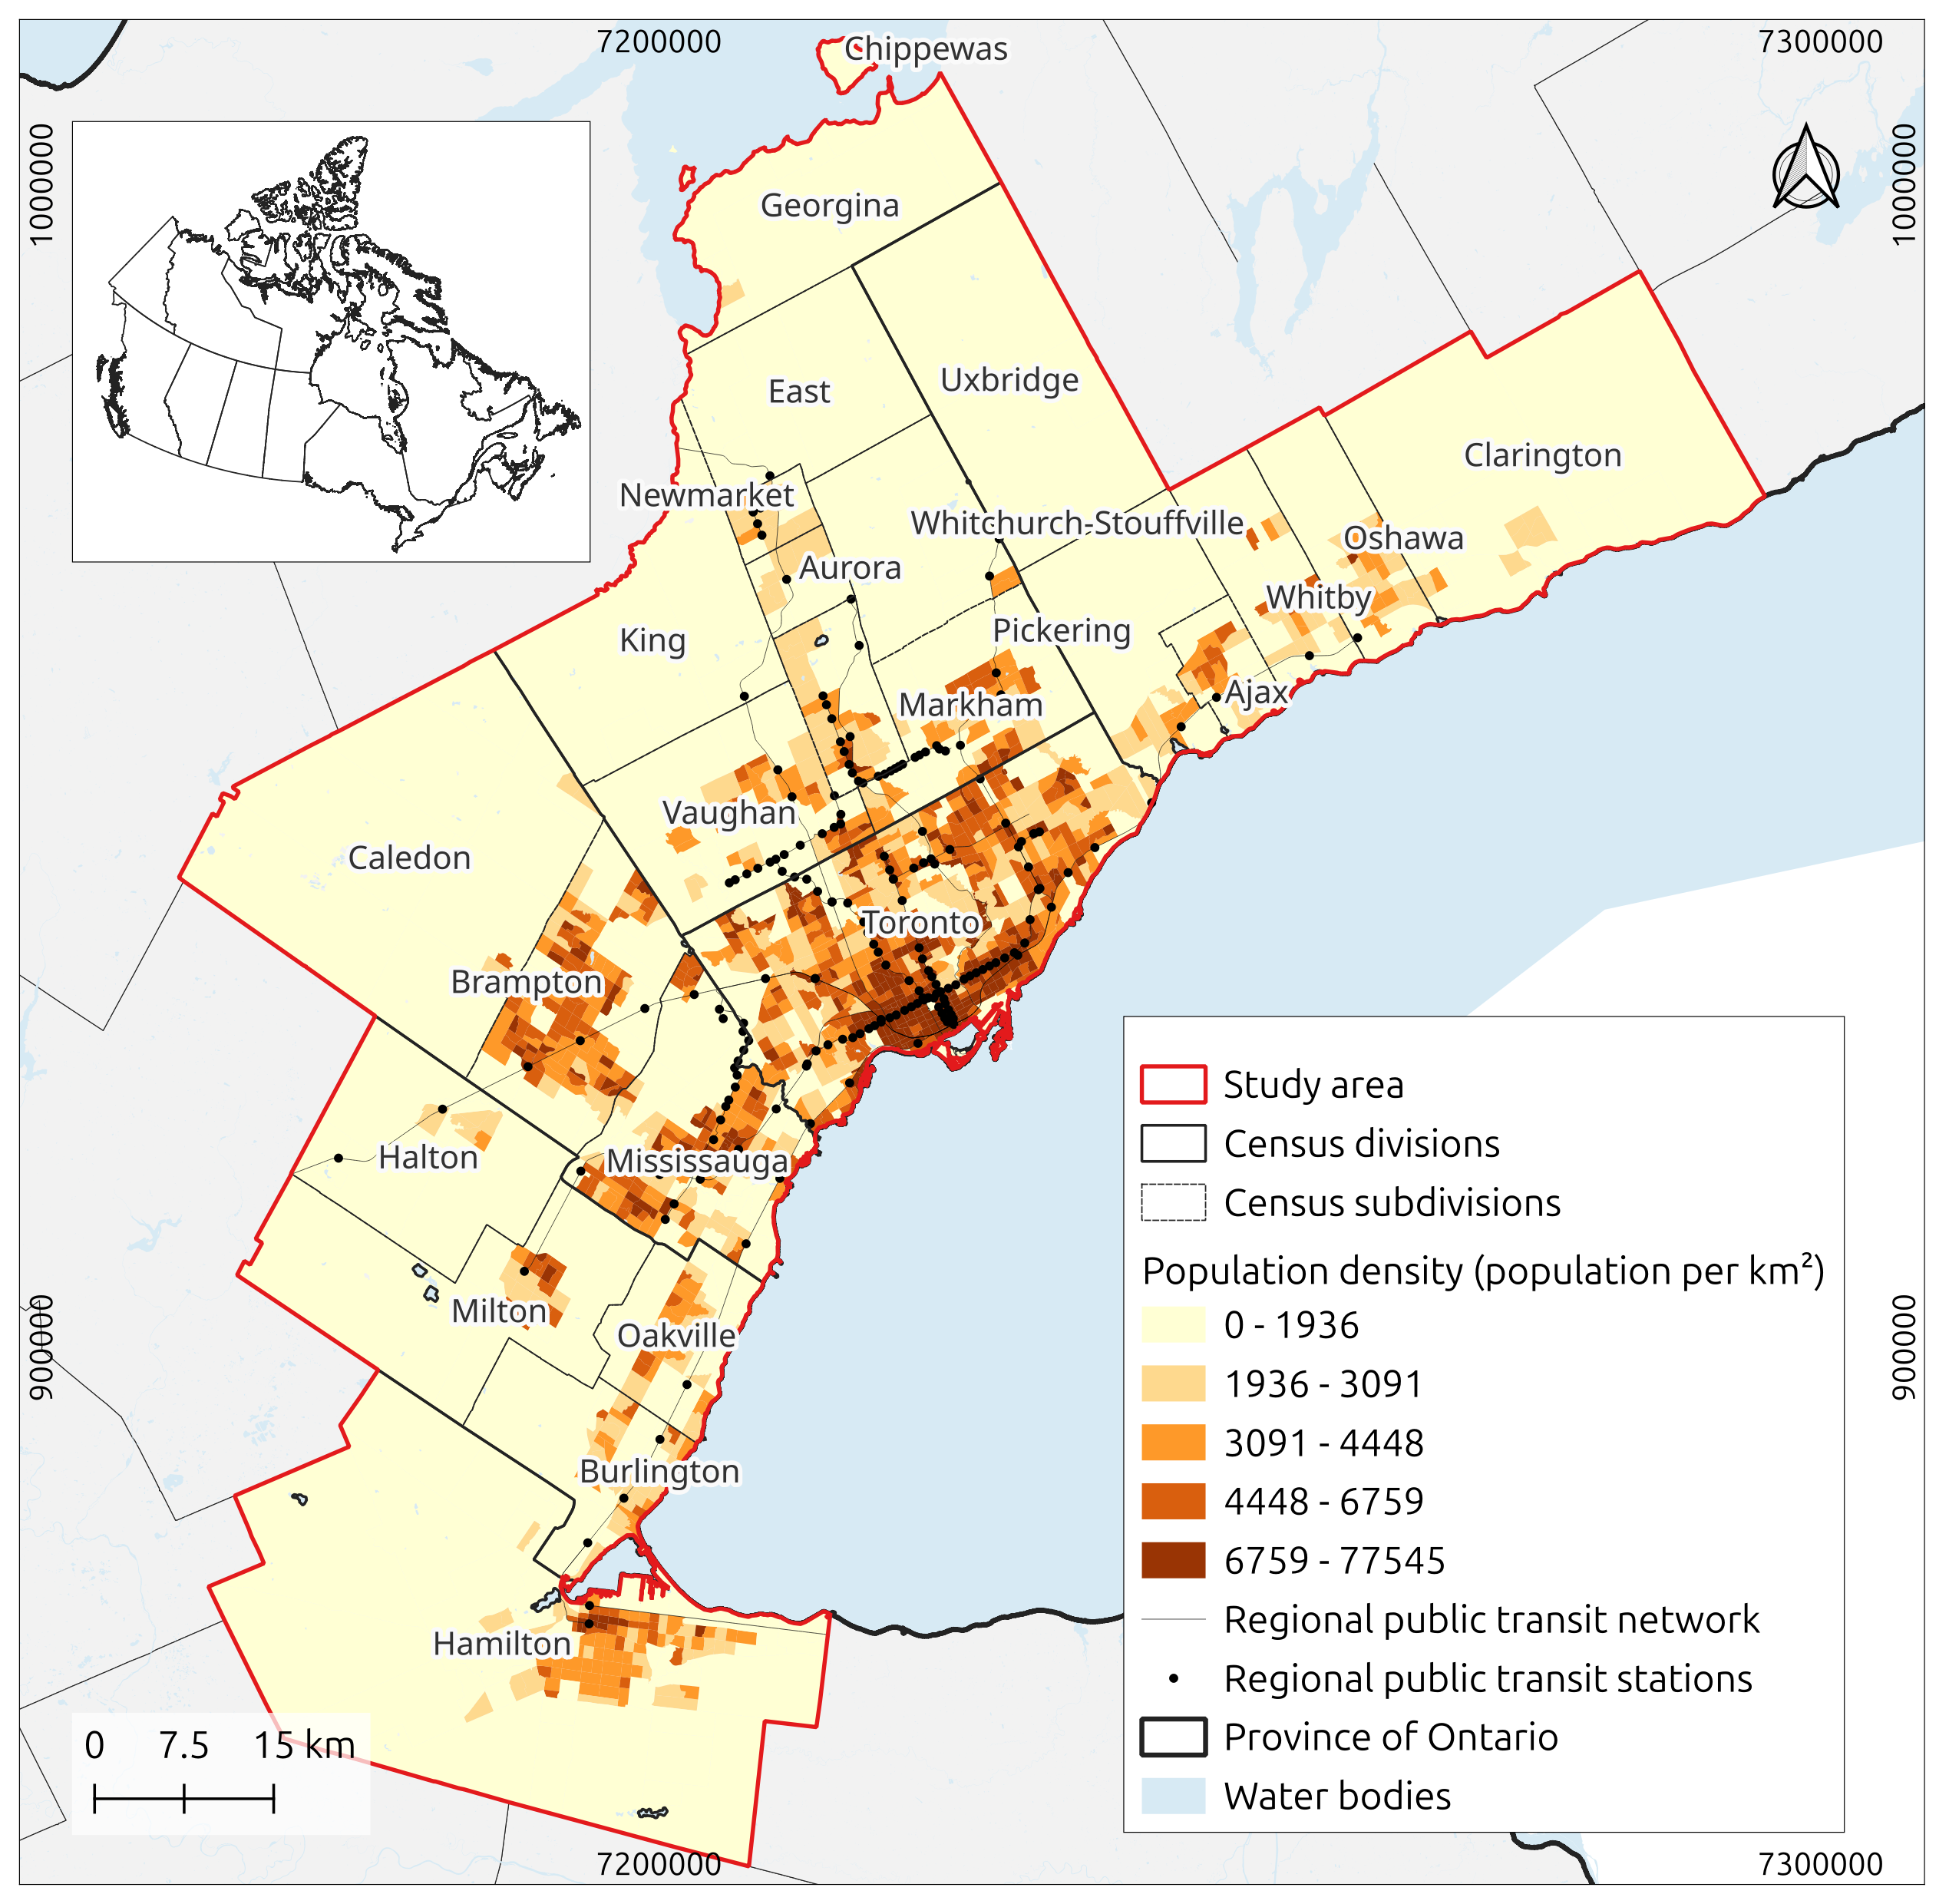
\includegraphics[width=1\linewidth]{figures/study_area_map} %%%
\DIFdelendFL \DIFaddbeginFL 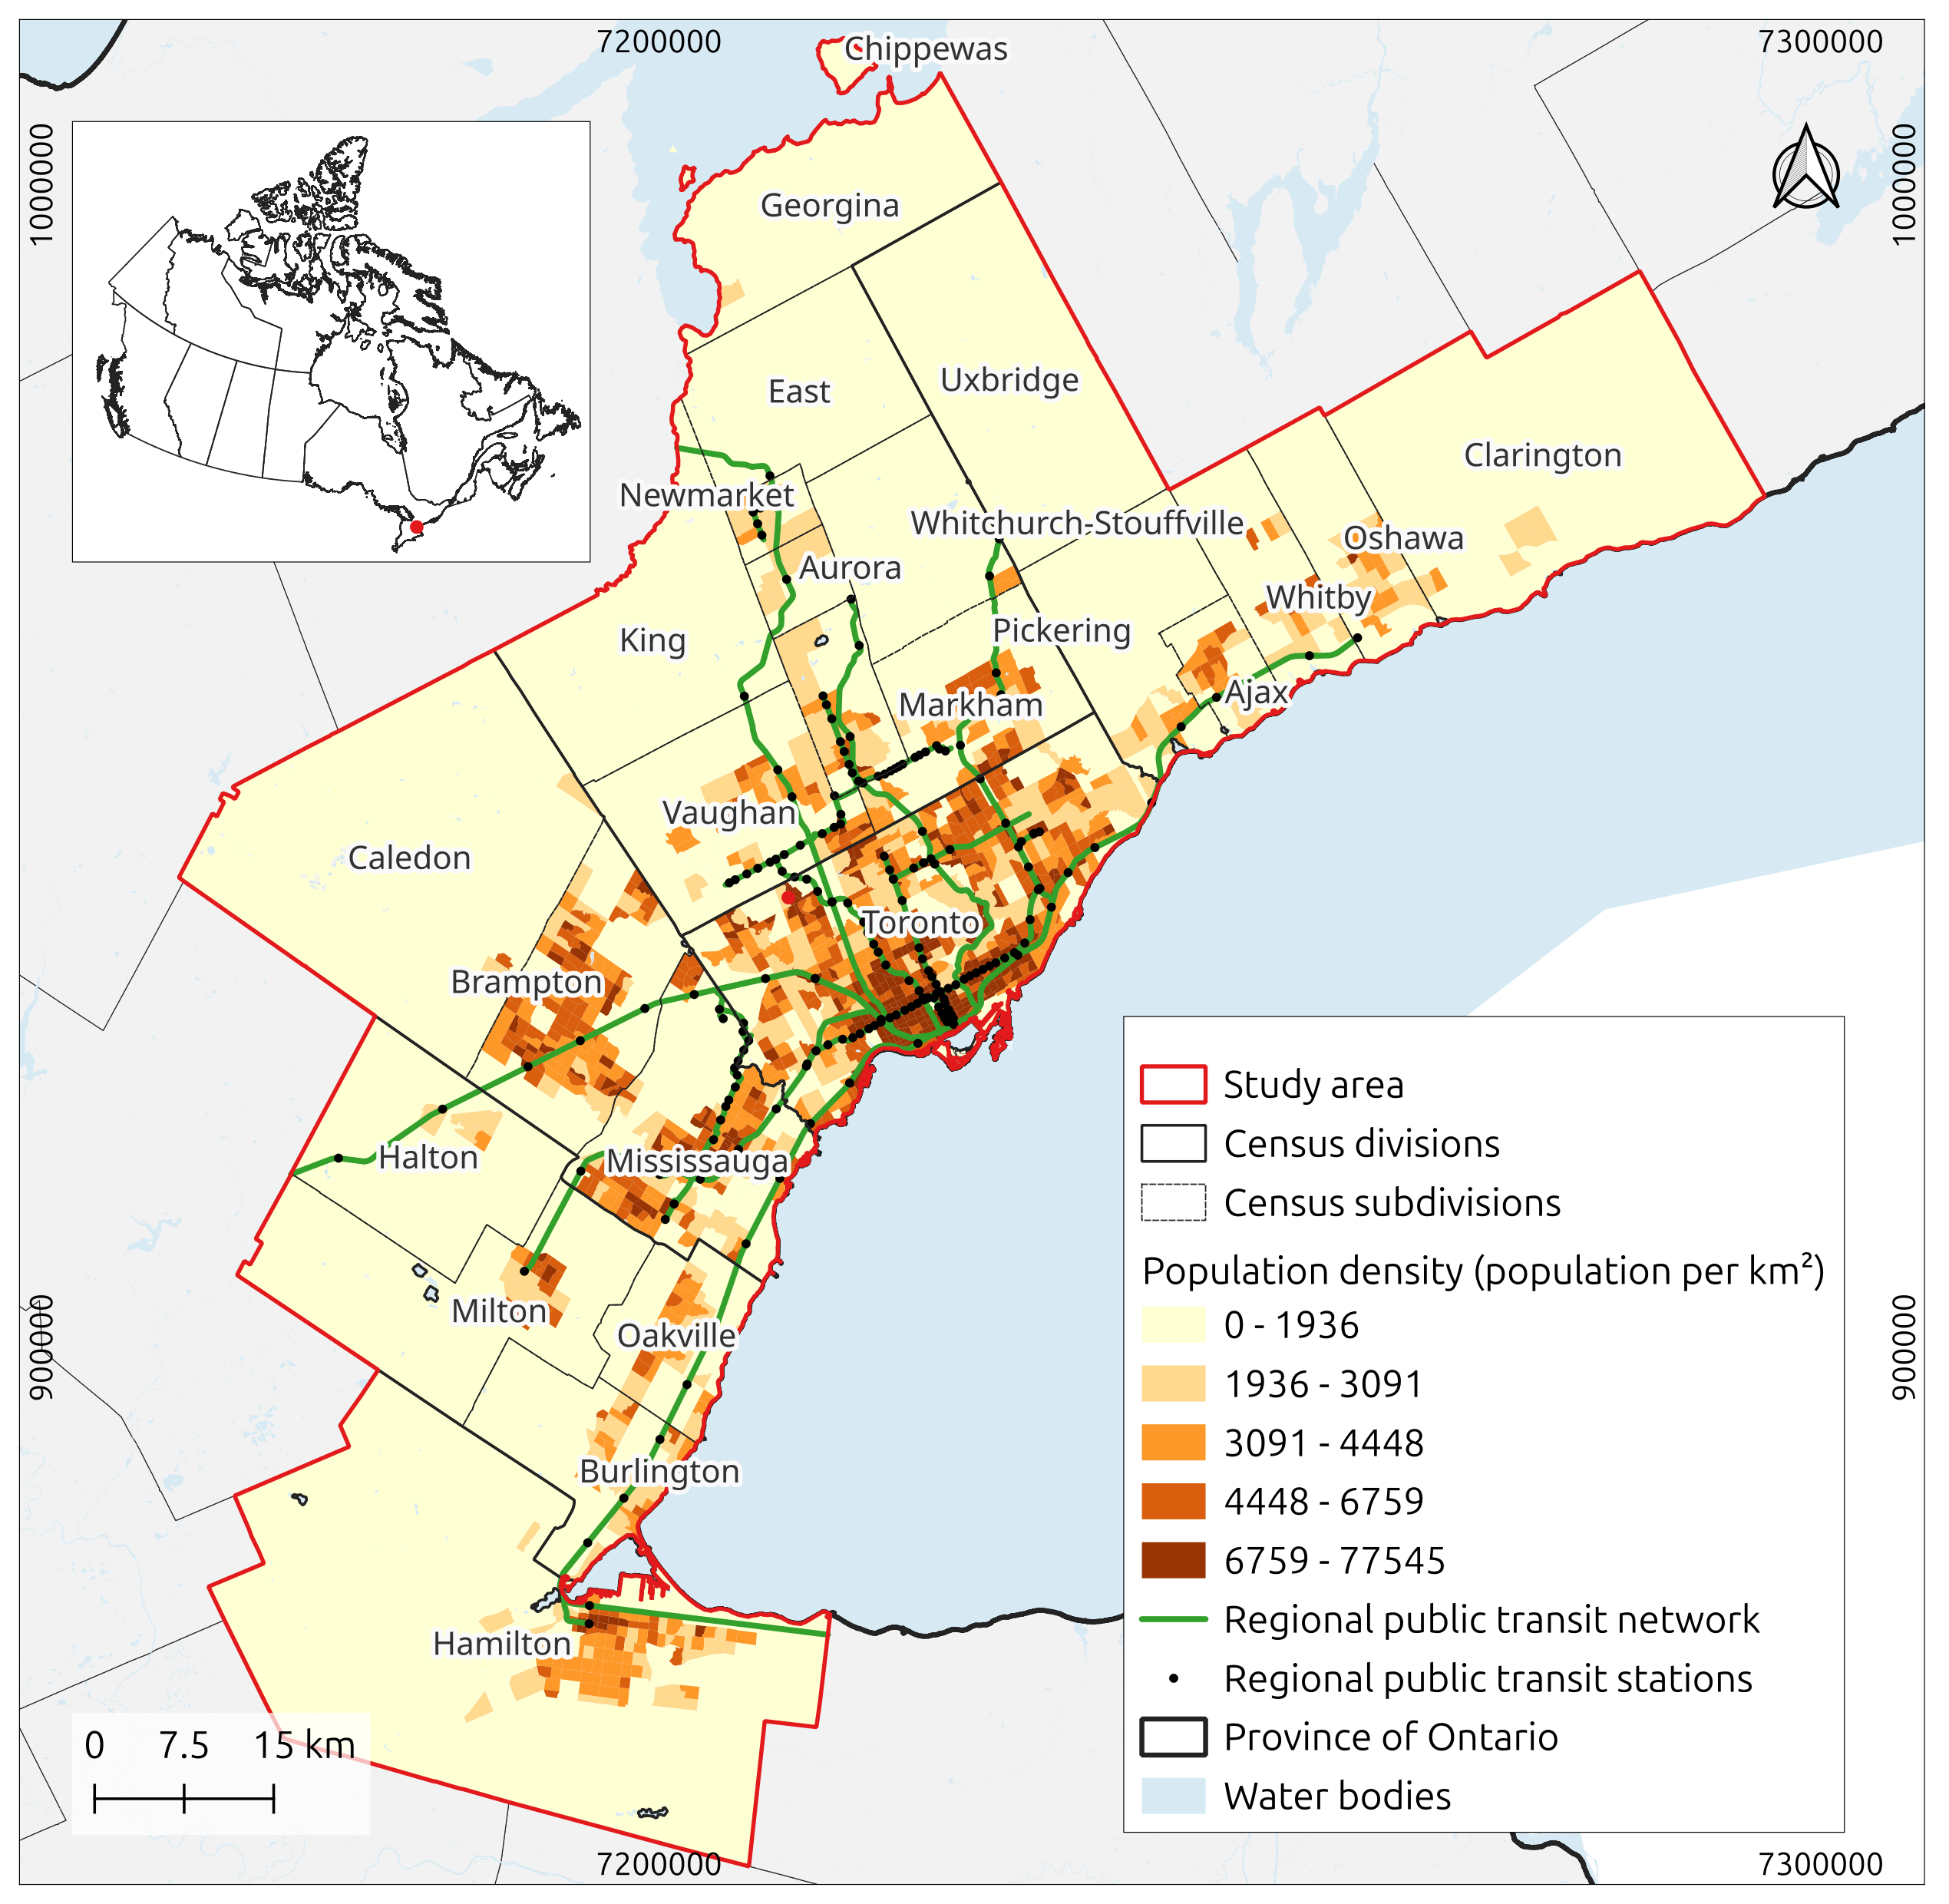
\includegraphics[width=1\linewidth]{figures/location_map_v2} \DIFaddendFL \caption{Map of the study area \DIFaddbeginFL \DIFaddFL{(population density is classified using quantile breaks)}\DIFaddendFL .}\label{fig:study-area-map}
\end{figure}

Regarding the primary data sources, this study uses data from two
different sources: the latest Canadian Census (2021) from Statistics
Canada; and the National Survey of Transport Poverty (NSTP) from the
Mobilizing Justice Partnership \citep{tiznado-aitken}. The Census was
selected due to its various socio-economic and demographic variables and
due to the ``Commuting to Work'' questionnaire, allowing the
identification of individuals in the labour force and including
variables required to calculate job accessibility, such as place of
work, commuting modes, and commuting duration. The Census also provides
standardized spatial datasets with statistical and administrative
geographical boundaries, including the Census Tract (CTs), which are
used in this study as the spatial units used for calculating
accessibility measures (obtained using the \DIFaddbegin \DIFadd{\{cancensus\} }\DIFaddend \texttt{\DIFdelbegin \DIFdel{cancensus}\DIFdelend \DIFaddbegin \DIFadd{R}\DIFaddend }
\DIFdelbegin \texttt{\DIFdel{R\ package}} %DIFAUXCMD
\DIFdelend \DIFaddbegin \DIFadd{package }\DIFaddend \citep{cancensus}). According to the Census
\citep{statisticscanada2023}, 3,868,120 individuals in the labour force
reside in the study area, competing for a total of 3,043,730 job
opportunities.

The second source of data, NSTP \citep{tiznado-aitken}, is a large-scale
survey designed to understand TRSE and transport poverty in Canada. It
is a representative sample of more than 27,000 people \DIFaddbegin \DIFadd{aged 15 years and
older }\DIFaddend across the country, and it provides an unprecedented \DIFdelbegin \DIFdel{perspective }\DIFdelend \DIFaddbegin \DIFadd{look }\DIFaddend at the
transportation challenges that Canadians face, especially among
\DIFdelbegin \DIFdel{equity-deserving }\DIFdelend \DIFaddbegin \DIFadd{transport-disadvantaged }\DIFaddend groups whose experiences are often overlooked.
The survey is openly available to researchers, decision-makers, and the
public, and offers information on household dynamics, respondents'
perceptions, and individual-level socioeconomic data. The NSTP provides
respondent weights to enable the creation of statistics that are
consistent and representative of the Canadian population. From this
survey we select variables corresponding to respondents' perceptions of
accessibility and employment outcomes, in addition to socioeconomic and
demographic variables at the individual level. The responses are
geocoded by place of residence and can be assigned to Census geographies
to link them to calculated accessibility.

Not all questions from the NSTP were answered by all survey respondents\DIFdelbegin \DIFdel{.
The questions were defined }\DIFdelend \DIFaddbegin \DIFadd{,
as questions were assigned }\DIFaddend according to demographic and socioeconomic
profiles and \DIFdelbegin \DIFdel{to }\DIFdelend previous responses. For this study, the NSTP sample
corresponds to \DIFaddbegin \DIFadd{labour force }\DIFaddend respondents residing in the GTHA who
\DIFaddbegin \DIFadd{reported being able to work, whether they are employed or unemployed,
and who are not retired, sick, or on parental leave, and who }\DIFaddend also
answered the questions displayed in Table \ref{tab:out-description},
totalling 2,270 respondents that represent 3,576,893 individuals in the
\DIFdelbegin \DIFdel{population
}\DIFdelend \DIFaddbegin \DIFadd{labour force }\DIFaddend (weighted sample). Using a continuum scale from 0
(completely disagree) to 100 (completely agree), the respondents
answered to what extent they agreed with the statements in Table
\ref{tab:out-description}.

\begin{table}
\centering
\caption{\label{tab:unnamed-chunk-1}\label{tab:out-description}Weighted summary statistics of the \DIFdelbeginFL \DIFdelFL{outcome }\DIFdelendFL \DIFaddbeginFL \DIFaddFL{dependent }\DIFaddendFL variables.}
\centering
\fontsize{10}{12}\selectfont
\begin{tabular}[t]{lc}
\toprule
To what extent do you agree with the following statements? & \textbf{N = 3,576,893}\\
\midrule
There are too few jobs available for me in my ideal commuting time & 58.84 (27.71)\\
I have had to decline employment opportunities because of my transport situation & 41.00 (31.62)\\
\bottomrule
\multicolumn{2}{l}{\rule{0pt}{1em}\textsuperscript{1} Mean (SD)}\\
\end{tabular}
\end{table}

\subsection{Calculating accessibility}\label{calculating-accessibility}

In this study, we implement the multimodal spatial availability measure
of \citet{soukhov2024}. This measure is a constrained indicator of
accessibility that can account for multiple modes
\citep[see][]{soukhov2023, soukhov2025}. This measure considers
competition for opportunities, which prevents a single job opportunity
to be available to more than one person. Competitive measures matter
when considering employment outcomes because jobs are exclusive, and
their use by one person prevents their use by another. In addition, this
measure relies on a proportional allocation that balances the cost of
travel and the population size, imposing a constrained calculation that
allocates the opportunities to each origin. This ensures that, when all
accessible jobs are summed, the sum is equal to the total number of
opportunities in the region. Lastly, this measure is a more
interpretable indicator since it returns scores in the units of
opportunities.

We calculated the multimodal spatial availability \(V_i^m\) using
Equation (\ref{eq:spatial-availability-multimodal}):

\begin{equation}
\label{eq:spatial-availability-multimodal}
V^m_{i} = \sum_{j=1}^J O_j\ F^{tm}_{ij}
\end{equation}

where:

\begin{itemize}
\tightlist
\item
  \(V^m_{i}\) is the spatial availability of opportunities at origin
  \(i\) and travel mode \(m\);
\item
  \(O_j\) is the number of opportunities at destination \(j\);
\item
  \(F^{tm}_{ij}\) is a balancing factor allocating opportunities at
  \(j\) to origin \(i\) considering mode \(m\).
\end{itemize}

\(F^{tm}_{ij}\) incorporates both population demand and travel
impedance, defined according to Equation
\ref{eq:multimodal-balancing-factors}:

\begin{equation}
\label{eq:multimodal-balancing-factors}
F^{tm}_{ij} = \frac{F^{pm}_{i} \cdot F^{cm}_{ij}}{\sum_{m=1}^M \sum_{i=1}^N F^{pm}_{i} \cdot F^{cm}_{ij}}
\end{equation}

The population-based allocation factor is obtained by:

\begin{itemize}
\tightlist
\item
  \(F^{pm}_{i} = \frac{P_{i}^m}{\sum_{m}\sum_{i} P_{i}^m}\)
\end{itemize}

Where \(P_{i}^m\) represents the population at origin \(i\) using mode
\(m\) \DIFdelbegin \DIFdel{. }\DIFdelend \DIFaddbegin \DIFadd{competing for the opportunities \(O\) at the destination \(j\). In
this study the population competing for these opportunities refers to
people in the labour force according to the classification used in the
Canadian Census.
}

\DIFaddend On its turn, the travel impedance allocation factor is given by:

\begin{itemize}
\tightlist
\item
  \(F_{ij}^{cm} = \frac{f^m(c_{ij}^m)}{\sum_{m} \sum_{i} f^m(c_{ij}^m)}\)
\end{itemize}

Where:

\begin{itemize}
\tightlist
\item
  \(c^m_{ij}\) is the cost to travel between \(i\) and \(j\) for mode
  \(m\);
\item
  \(f^m{c^m_{ij}}\) is an impedance function representing the effect of
  travel cost.
\end{itemize}

Using microdata from the Census, we calculated for each CT the number of
people in the labour force that commute to work by walking, cycling,
\DIFdelbegin \DIFdel{motorized modes }\DIFdelend \DIFaddbegin \DIFadd{private vehicles }\DIFaddend (those who commute by car, truck, or van as a driver or
passenger, and motorcycles or scooters), and public transit (those who
commute by bus, subway, light rail, streetcar, commuter train, and
passenger ferry). We distributed remote workers according to the share
of each transportation mode in each CT. Then, we summed the number of
jobs in each CT considering the place of work mentioned by each worker.

We calculated the travel times between origins and destinations for each
travel mode using the \{r5r\} \texttt{R} package \citep{pereira2021a}
with a street network obtained from OpenStreetMap. We used the General
Transit Feed Specification (GTFS) obtained from the Canadian Public
Transit Network Database \citep{statisticscanada} to retrieve the public
transit schedule and coverage. Considering that our study area contains
different transit agencies, we evaluated the GTFS files to identify a
common date/week with public transit service. After this analysis, we
set 8 a.m. (morning peak time) of December 22, 2025, as the trip
departure time. Although this date falls during Christmas week, there
were no differences in the public transit service schedules of the
transit agencies due to the holiday, which makes this date
representative of a regular weekday in terms of public transit travel
time estimation. We also used Digital Elevation Models (DEM) from the
Canadian Digital Surface Model (CDSM), with a spatial resolution of
about 20 meters, to estimate the effect of declivity on walking and
cycling times. \DIFaddbegin \DIFadd{For cycling trips, we defined a standard level of traffic
stress (LTS) as tolerable for most mainstream adults. LTS defines the
level of comfort or danger that a street presents for cyclists based on
speed limits, lane counts, and infrastructure. The standard LTS defined
in \{r5r\} \mbox{%DIFAUXCMD
\citep{pereira2021a} }\hskip0pt%DIFAUXCMD
includes bike lanes with physical
separation from multi-lane or higher-speed traffic. }\DIFaddend We set a maximum
duration of 180 minutes (3 hours) for \DIFdelbegin \DIFdel{motorized }\DIFdelend \DIFaddbegin \DIFadd{private vehicles }\DIFaddend and public
transit trips, with a maximum walking time of 5 minutes to reach the
vehicle and 15 minutes to reach the public transit stop/station; for
walking and cycling trips, we set a maximum duration of 90 minutes (one
and a half hours). After estimating the travel times between CTs, we
assumed that all intra-CT trip durations are equal to 0.1 minute.

Commute duration was used to calibrate Probability Density Functions
(PDFs) to represent travel impedance, following the approach of Soukhov
and Páez \citeyearpar{soukhov2024a}, Verma and Ukkusuri
\citeyearpar{verma2025}, and Dos Santos et al.
\citeyearpar{dossantos2026}, where the impedance value represents the
probability that the trip will occur given a \DIFdelbegin \DIFdel{specif }\DIFdelend \DIFaddbegin \DIFadd{specific }\DIFaddend travel time. We
used the \{\DIFdelbegin \DIFdel{fitdistrplu\} s }\DIFdelend \DIFaddbegin \DIFadd{fitdistrplus\} }\DIFaddend \texttt{R} package
\citep{delignette-muller2015} and tested different functional forms
(uniform, negative exponential, gamma, normal, and lognormal
distributions) to select the best PDF for each mode of transportation
and municipality, using \DIFdelbegin \DIFdel{a }\DIFdelend \DIFaddbegin \DIFadd{as the }\DIFaddend selection criteria the lowest Akaike
Information Criterion (AIC) value \citep{akaike1974}. The estimated
impedance functions appear in Table \ref{tab:impedance_functions}.

\subsection{Modeling the \DIFdelbegin \DIFdel{causal }\DIFdelend relationship between calculated \DIFdelbegin \DIFdel{and
}\DIFdelend \DIFaddbegin \DIFadd{accessibility,
}\DIFaddend perceived accessibility\DIFaddbegin \DIFadd{, and employment
outcomes}\DIFaddend }\DIFdelbegin %DIFDELCMD < \label{modeling-the-causal-relationship-between-calculated-and-perceived-accessibility}
%DIFDELCMD < %%%
\DIFdelend \DIFaddbegin \label{modeling-the-relationship-between-calculated-accessibility-perceived-accessibility-and-employment-outcomes}
\DIFaddend 

In this study, we aim to define minimum levels of calculated
accessibility by identifying key thresholds in its relationship with
perceived accessibility \DIFaddbegin \DIFadd{and employment outcomes}\DIFaddend . The underlying
\DIFdelbegin \DIFdel{assumption }\DIFdelend \DIFaddbegin \DIFadd{hypothesis }\DIFaddend of this strategy is that \DIFdelbegin \DIFdel{there is a connection between these two components of
accessibility, such that changes in calculated }\DIFdelend \DIFaddbegin \DIFadd{changes in the land-use and
transport characteristics of a neighbourhood, captured and represented
by calculated accessibility, lead to changes in how residents perceives
their ability to reach job opportunities and in their reported
employment outcomes. We hypothesize that residents of neighbourhoods
with more (calculated) }\DIFaddend accessibility \DIFdelbegin \DIFdel{would
result on changes in the distribution of perceived accessibility. This
implies a causal relationship between calculated (the cause or the
treatment) and perceived accessibility (the outcome), rather than merely
their statistical correlation. Therefore, we hypothesise that higher
values of calculated accessibility
will increase the probability of
being in more positive perception categories, and that perceptions of
accessibility can be connected to multimodal spatial availability
indicators}\DIFdelend \DIFaddbegin \DIFadd{are less likely to perceive job
scarcity or to report having declined employment due to transport
constraints, independent of their individual demographic and
socioeconomic profiles. In our approach, we use calculated accessibility
not as a causal exposure in itself, but as a proxy for the underlying
land-use and transport conditions that, as we hypothesize, shape
individual perceptions and outcomes}\DIFaddend .

Following the steps suggested by Huntington-Klein
\citeyearpar{huntington-klein2021}, we draw a \DIFdelbegin \DIFdel{causal diagram }\DIFdelend \DIFaddbegin \DIFadd{Directed Acyclic Graph
(DAG) }\DIFaddend to graphically represent \DIFdelbegin \DIFdel{the assumed causal relationship between calculated
and perceived accessibility }\DIFdelend \DIFaddbegin \DIFadd{our hypothesis }\DIFaddend (Figure \ref{fig:DAG}).
\DIFdelbegin \DIFdel{Causal diagrams }\DIFdelend \DIFaddbegin \DIFadd{DAGs }\DIFaddend show a chain of \DIFaddbegin \DIFadd{hypothesized }\DIFaddend causal effects by using nodes to
symbolize random variables and arrows to represent the causal effect
between two random variables in the direction of the arrow
\citep{cunningham2021causal}.

\begin{figure}
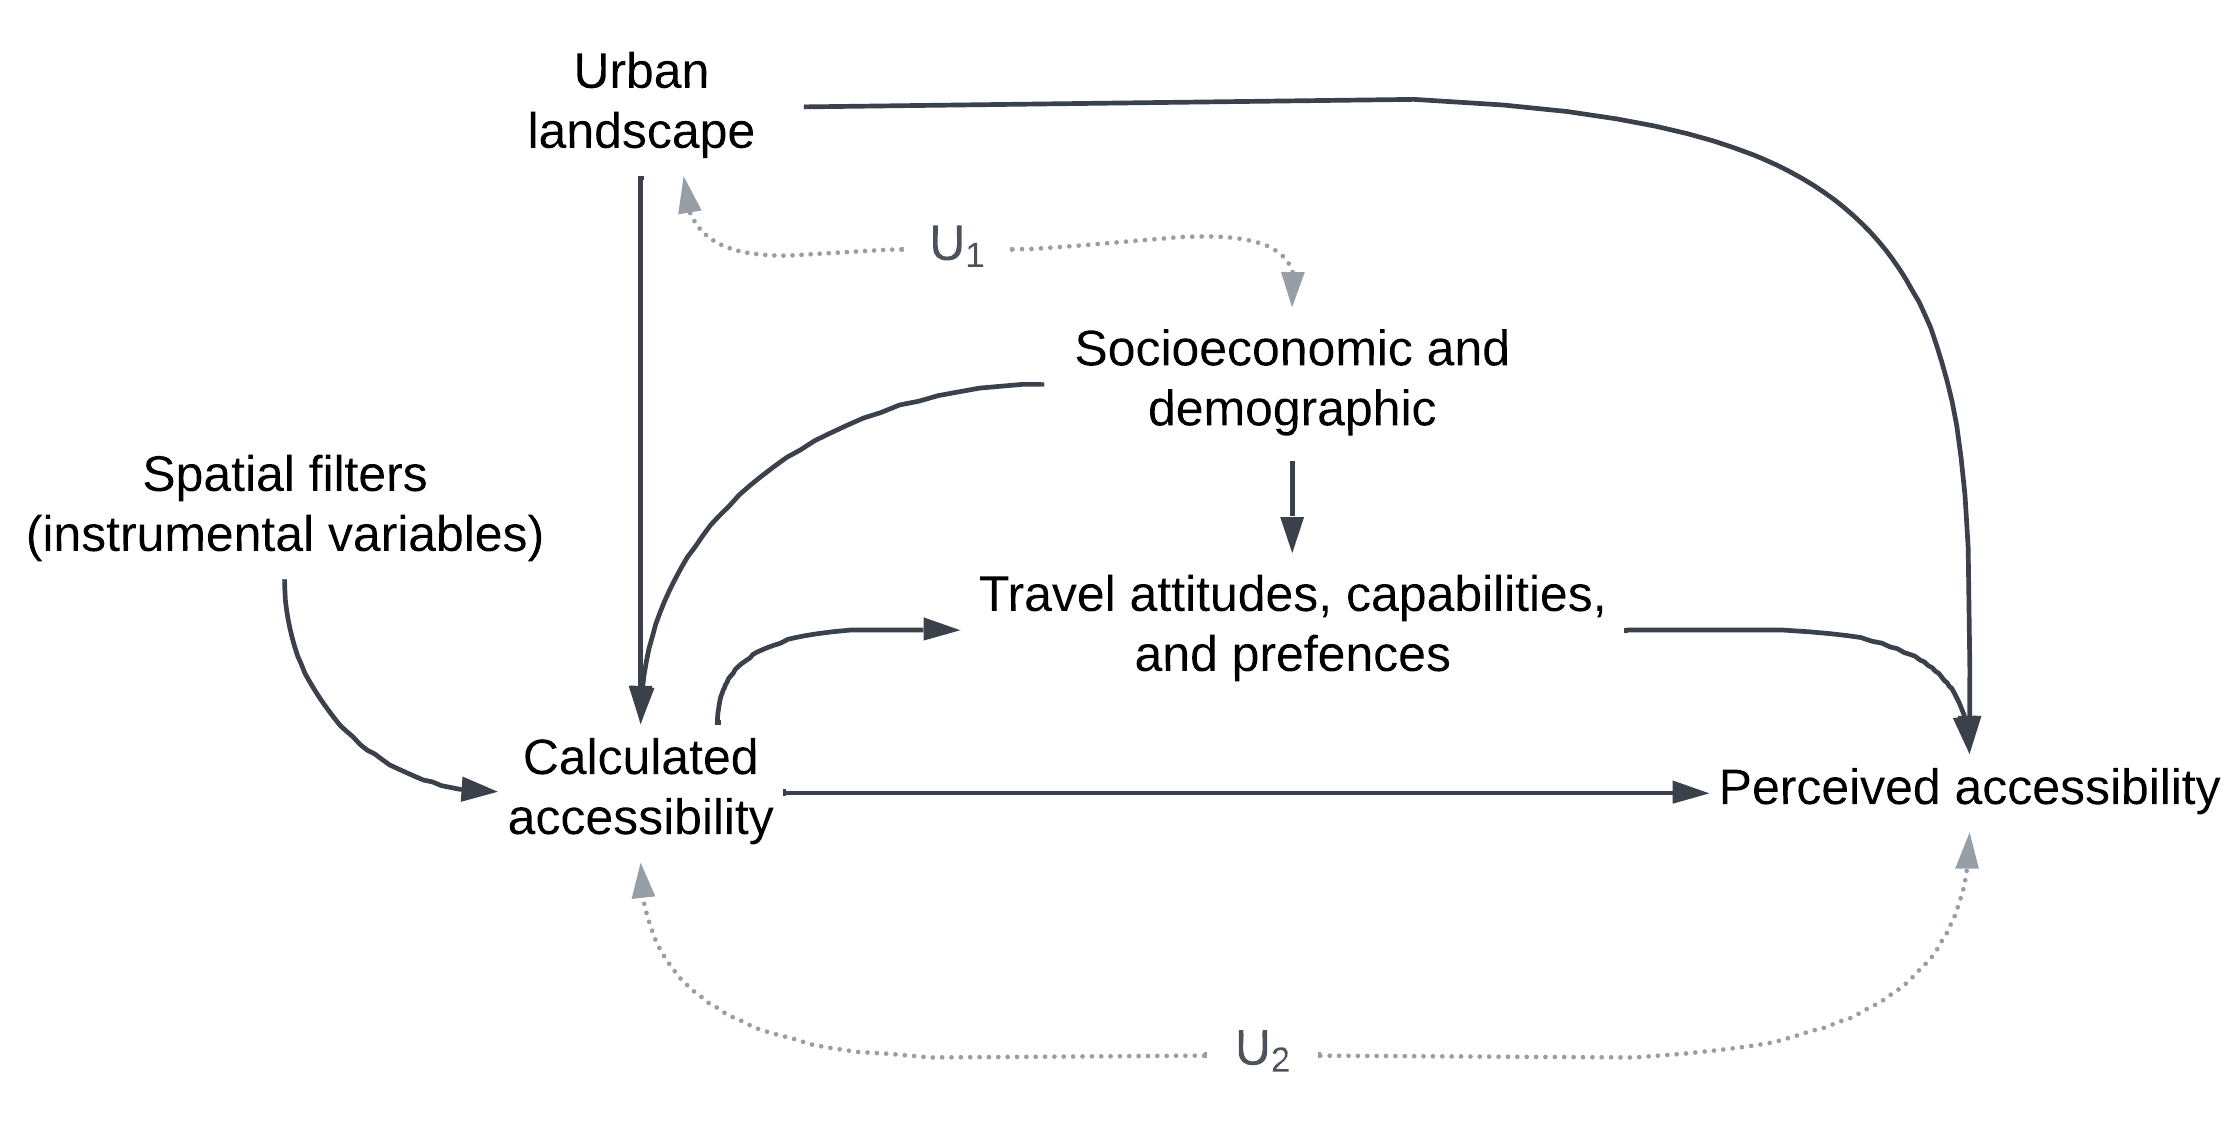
\includegraphics[width=1\linewidth]{figures/DAG} \caption{\DIFdelbeginFL \DIFdelFL{Causal diagram }\DIFdelendFL \DIFaddbeginFL \DIFaddFL{Directed acyclic graph (DAG) }\DIFaddendFL of calculated accessibility on perceived accessibility.}\label{fig:DAG}
\end{figure}

\DIFdelbegin \DIFdel{According to our diagram, }\DIFdelend \DIFaddbegin \DIFadd{We hypothesize that }\DIFaddend there is a \DIFdelbegin \DIFdel{direct effect of calculated accessibility on perceived accessibility}\DIFdelend \DIFaddbegin \DIFadd{association between calculated job
accessibility, perceived accessibility, employment outcomes}\DIFaddend . However,
there are other ways in which they are connected\DIFaddbegin \DIFadd{, represented by the
other nodes of the diagram}\DIFaddend . First, there are mediator components that
influence the way a person perceives\DIFdelbegin \DIFdel{calculated accessibility. In our
study, we use place-based measures to calculate accessibility, so that
these indicators represent neighbourhood characteristics (CT level). However, each individual will perceive these }\DIFdelend \DIFaddbegin \DIFadd{, or make use of, calculated
accessibility. Each individual perceives the same }\DIFaddend neighbourhood
characteristics differently based on their capabilities and preferences,
as well as their travel options and experiences. For instance, a person
with a disability that prevents or makes it difficult for them to walk
or cycle will probably not enjoy the benefits of active accessibility to
the same extent as a person without such a disability
\citep{church_accessibility_2003}; someone without a car will not take
advantage of high car accessibility; someone without a monthly transit
pass might take less public transit than someone with a transit pass,
therefore reducing their potential for spatial interaction promoted by
higher public transit accessibility.

In \DIFdelbegin \DIFdel{the causal diagram, the accessibility of a neighbourhood is caused by
urban characteristics, such as land use and transportation
infrastructure. In }\DIFdelend addition, place of residence, and consequently \DIFdelbegin \DIFdel{their
}\DIFdelend \DIFaddbegin \DIFadd{an individual's
}\DIFaddend neighbourhood accessibility, is \DIFdelbegin \DIFdel{affected (caused) }\DIFdelend \DIFaddbegin \DIFadd{also influenced }\DIFaddend by socioeconomic
factors, with household income as the main driver of this decision, and
also by demographic characteristics (such as gender, race, citizenship,
among others). These socioeconomic and demographic factors not only
\DIFdelbegin \DIFdel{determine }\DIFdelend \DIFaddbegin \DIFadd{influence }\DIFaddend where someone will live, but also shape how individuals
experience travel and, consequently, make use of their neighbourhood
accessibility.

However, \DIFdelbegin \DIFdel{it is also worth mentioning that }\DIFdelend socioeconomic and demographic factors and the urban landscape
of \DIFaddbegin \DIFadd{the }\DIFaddend place of residence are also linked through a common cause
(\(U_1\)) that we cannot measure \DIFdelbegin \DIFdel{or properly
define as a variable causing both. For instance,
}\DIFdelend \DIFaddbegin \DIFadd{directly, such as generational wealth,
which likely influences both }\DIFaddend someone's neighbourhood and their income
level\DIFdelbegin \DIFdel{are probably related to generational wealth, a
variable that cannot be obtained from the surveys. In addition, there
must exist other factors, unknown or not translated into measurable
variables, that probably affect both calculated and perceived
accessibility(\(U_1\)}\DIFdelend \DIFaddbegin \DIFadd{. Other unmeasured factors, such as residential self-selection and
adaptive preference, likely affect calculated accessibility, perceived
accessibility, and employment outcomes (\(U_2\)}\DIFaddend ).

\DIFdelbegin \DIFdel{From a causal diagram, we can identify all paths through which we can go
from one node (a variable) to another using the arrows connecting them, with particular importance given to those paths connecting the treatment
to }\DIFdelend \DIFaddbegin \DIFadd{Because other paths link calculated accessibility to perceived
accessibility and employment outcomes, }\DIFaddend the \DIFdelbegin \DIFdel{outcome. Paths in which all arrows point away from the treatment
are front-door paths \mbox{%DIFAUXCMD
\citep{cunningham2021causal, huntington-klein2021}}\hskip0pt%DIFAUXCMD
;
whereas paths that point towards the treatment are back-door paths. To
identify the effect of the treatment on
the outcome, we need to control
for at least one variable in the back-door paths (hold this variable
constant and unchanged), in a process that closes these biasing paths,
while not controlling for at least one front-door path
\mbox{%DIFAUXCMD
\citep{huntington-klein2021}}\hskip0pt%DIFAUXCMD
. In this study, we employ regressions to estimate the relationship between treatment and outcome, }\DIFdelend \DIFaddbegin \DIFadd{observed association between
them cannot be assumed to reflect the true effect of accessibility on
how people experience and evaluate their access to employment
opportunities. If calculated accessibility is to be used as a benchmark
or standard for equitable transportation planning, we believe it is
important to apply methods that aim to isolate its association with
perceived accessibility and employment outcomes, after accounting for
these confounding mechanisms, instead of relying on a raw statistical
association that may be inflated, offset, or masked by unobserved
individual preferences and constraints. Our approach relies on, first,
}\DIFaddend controlling for \DIFdelbegin \DIFdel{all other measurable variables.
}%DIFDELCMD < 

%DIFDELCMD < %%%
\DIFdel{To model the causal diagram from Figure \ref{fig:DAG}, we use weighted
regressions that combine multimodal spatial availability per person with
variables at the individual and household levels from the NSTP. Considering respondent weights, we transformed the perception variables
into an ordered Likert scale based ontheir quintile position, categorizing them as: ``Most Negative'', ``Negative'',
``Neutral'',
``Positive'', and ``Most Positive''. The thresholds used for this
categorization is presented in Table \ref{tab:outcomes_quintiles}}\DIFdelend \DIFaddbegin \DIFadd{individual-level covariates capturing demographic,
socioeconomic, and travel-related characteristics; and second, applying
a framework using instrumental variables}\DIFaddend .

\DIFdelbegin %DIFDELCMD < \begin{table}
%DIFDELCMD < \centering
%DIFDELCMD < %%%
%DIFDELCMD < \caption{%
{%DIFAUXCMD
%DIFDELCMD < \label{tab:outcomes-quintiles}\label{tab:outcomes_quintiles}%%%
\DIFdelFL{Quintile thresholds used to categorize outcomes.}}
%DIFAUXCMD
%DIFDELCMD < \centering
%DIFDELCMD < \fontsize{10}{12}\selectfont
%DIFDELCMD < \begin{tabular}[t]{lrrrrr}
%DIFDELCMD < \toprule
%DIFDELCMD < Outcome & 20\% & 40\% & 60\% & 80\% & 100\%\\
%DIFDELCMD < \midrule
%DIFDELCMD < Few jobs available & 35 & 52 & 69 & 87 & 100\\
%DIFDELCMD < Decline employment & 8 & 26 & 51 & 72 & 100\\
%DIFDELCMD < \bottomrule
%DIFDELCMD < \end{tabular}
%DIFDELCMD < \end{table}
%DIFDELCMD < 

%DIFDELCMD < %%%
\DIFdel{Based on the causal diagram and on our literaturereview, we selected
the following variables to represent each node}\DIFdelend \DIFaddbegin \DIFadd{Guided by the diagram and the supporting literature, we identified
control variables corresponding to each node, following standard
causal-diagram identification methods
\mbox{%DIFAUXCMD
\citep{cunningham2021causal, huntington-klein2021}}\hskip0pt%DIFAUXCMD
. We selected the
following variables}\DIFaddend :

\begin{itemize}
\tightlist
\item
  Calculated accessibility (treatment): multimodal spatial availability
  per person \DIFdelbegin \DIFdel{(active, public transit, and motorized modes)}\DIFdelend \DIFaddbegin \DIFadd{by transportation mode}\DIFaddend .
\item
  Perceived accessibility (outcome \DIFdelbegin \DIFdel{): individual perceptions categorized
  on a Likert scale, obtained
  from NTSP}\DIFdelend \DIFaddbegin \DIFadd{1): agreement with }\emph{\DIFadd{``there are
  too few jobs available for me in my ideal commuting time,''}} \DIFadd{obtained
  from NSTP.
}\item
  \DIFadd{Self-reported employment outcome (outcome 2): agreement with }\emph{\DIFadd{``I
  have had to decline employment opportunities because of my transport
  situation,''}} \DIFadd{obtained from NSTP}\DIFaddend .
\item
  Travel attitudes, capabilities, and prefences: most used
  transportation mode; whether the preferred transportation mode matches
  the most frequent mode; whether the individual has a monthly or annual
  public transit pass; number of cars and bikes in the household; and
  whether the person has any disability, all obtained from \DIFdelbegin \DIFdel{NTSP}\DIFdelend \DIFaddbegin \DIFadd{NSTP}\DIFaddend .
\item
  Socioeconomic and demographic: whether the person is Indigenous or
  from a racialized population group; whether the person self-identifies
  as a woman; or as a transgender or non-binary person; age; household
  size and household income; and citizenship (temporary visa or
  refugee), all obtained from \DIFdelbegin \DIFdel{NTSP}\DIFdelend \DIFaddbegin \DIFadd{NSTP}\DIFaddend .
\item
  Urban landscape: population centre class (rural, small, medium, or
  large urban population centre) and population density (dissemination
  area level), obtained from Census.
\end{itemize}

\DIFaddbegin \DIFadd{We use weighted regressions that combine multimodal spatial availability
per person with variables at the individual and household levels from
the NSTP. Considering respondent weights, we transformed the dependent
variables into an ordered Likert scale based on their quintile position,
categorizing them as: ``Most Negative'', ``Negative'', ``Neutral'',
``Positive'', and ``Most Positive''. The thresholds used for this
categorization are presented in Table \ref{tab:outcomes_quintiles}.
}

\begin{table}
\centering
\caption{\label{tab:outcomes-quintiles}\label{tab:outcomes_quintiles}\DIFaddFL{Quintile thresholds used to categorize dependent variables.}}
\centering
\fontsize{10}{12}\selectfont
\begin{tabular}[t]{lrrrrr}
\toprule
Outcome & 20\% & 40\% & 60\% & 80\% & 100\%\\
\midrule
Few jobs available in my ideal commuting time & 35 & 52 & 69 & 87 & 100\\
Declined employment opportunities because of my transport situation & 8 & 26 & 51 & 72 & 100\\
\bottomrule
\end{tabular}
\end{table}

\DIFaddend Considering that the outcome is an ordinal categorical variable, we used
weighted ordinal logistic regressions \citep{lumley2011} to model the
\DIFdelbegin \DIFdel{effect of }\DIFdelend \DIFaddbegin \DIFadd{relationship between }\DIFaddend the calculated accessibility indicators \DIFdelbegin \DIFdel{on the
perception
categories }\DIFdelend \DIFaddbegin \DIFadd{and the
categories of the dependent variables}\DIFaddend , using Equation
\ref{eq:ordinal-logit}:

\begin{equation}
\label{eq:ordinal-logit}
\log(\frac{P(Y\le j)}{P(Y\ge j)}) = \theta_j - \beta_1 X_1 + \beta_2 X_2 + ... + \beta_p X_p
\end{equation}

\noindent where \(Y\) represents the perception category of the
respondent (ranging from ``Most Negative'' to ``Most Positive''), and
\(X_1, X2, ..., X_p\) represent the set of explanatory variables, and
\(\theta_j\) and \(\beta_p\) are unknown parameters to be estimated. The
parameters \(\beta_p\) are constant for all outcome categories and
measure the change in the log-odds of reporting higher perception
categories associated with each explanatory variable, while \(\theta_j\)
represents the intercept separating the perception categories.
\DIFaddbegin 

\begin{table}

\caption{\label{tab:vardescriptions}\label{tab:var-description}\DIFaddFL{Weighted summary statistics of the explanatory variables, based on the NSTP respondents in the labour force and residing in the Greater Toronto and Hamilton Area.}}
\centering
\begin{tabular}[t]{lc}
\toprule
Explanatory variables & \textbf{N = 3,576,893}\\
\midrule
Active job accessibility per active traveller & 0.06 (0.13)\\
Transit job accessibility per transit user & 0.14 (0.09)\\
Private vehicle accessibility per user & 1.00 (0.27)\\
Active commuter & 528,927 (15\%)\\
Public transit user & 829,940 (23\%)\\
\addlinespace
Person with disability & 716,861 (20\%)\\
Number of Cars & 1.30 (0.92)\\
Number of Bikes & 1.15 (1.33)\\
Preferred mode match most frequent mode & 2,706,882 (76\%)\\
Indigenous or racialized person & 1,866,043 (52\%)\\
\addlinespace
Temporary visa or refugee & 268,654 (7.5\%)\\
Woman, transgender or non-binary person & 1,757,263 (49\%)\\
Age & 40.15 (13.49)\\
Household size & 2.90 (1.61)\\
Household income & \\
\addlinespace
\hspace{1em}Less than \$40,000 & 561,182 (16\%)\\
\hspace{1em}\$40,000 to \$80,000 & 1,145,633 (32\%)\\
\hspace{1em}\$80,000 to \$120,000 & 930,128 (26\%)\\
\hspace{1em}More than \$120,000 & 939,950 (26\%)\\
Population density (people/km2) & 7,809.82 (13,610.23)\\
\addlinespace
Population centre class & \\
\hspace{1em}Rural & 89,251 (2.5\%)\\
\hspace{1em}Small & 48,306 (1.4\%)\\
\hspace{1em}Medium & 58,128 (1.6\%)\\
\hspace{1em}Large & 3,381,208 (95\%)\\
\addlinespace
Public transit availability in the neighbourhood & 3,435,002 (96\%)\\
Monthly or annual public transit pass & 1,063,225 (30\%)\\
\bottomrule
\multicolumn{2}{l}{\rule{0pt}{1em}\textsuperscript{1} Mean (SD); n (\%)}\\
\end{tabular}
\end{table}

\DIFadd{Because of the high correlation between public transit and bicycle
accessibility (with Pearson correlation above 0.80), and because only 61
NSTP respondents (less than 3\% of the sample) mentioned cycling as
their main commuting mode, we combined walking and cycling into a single
active transportation indicator, summing the jobs spatially available by
each mode. Including bicycle accessibility as a separate indicator,
given this small subsample and high collinearity with transit
accessibility, would likely have caused convergence problems when
creating our ordinal models. Fitting these models also requires a
sufficient number of respondents within each category and combination of
categories, which the small cycling subsample could not support.
However, we acknowledge that this combined active measure does not
account for the difference in travel speed between walking and cycling,
which can be substantial, and may understate the accessibility gains
cycling offers relative to walking over longer distances.
}

\DIFaddend Table \ref{tab:var-description} presents the variables included in the
regression models and their descriptive statistics \DIFaddbegin \DIFadd{for the NSTP sample
}\DIFaddend (weighted mean and weighted standard deviation for continuous and dummy
variables, and weighted count and percentage for categorical variables,
created using the \{gtsummary\} \texttt{R} package \citep{gtsummary}).

\DIFdelbegin %DIFDELCMD < \begin{table}
%DIFDELCMD < 

%DIFDELCMD < %%%
%DIFDELCMD < \caption{%
{%DIFAUXCMD
%DIFDELCMD < \label{tab:vardescriptions}\label{tab:var-description}%%%
\DIFdelFL{Weighted summary statistics of the explanatory variables.}}
%DIFAUXCMD
%DIFDELCMD < \centering
%DIFDELCMD < \begin{tabular}[t]{lc}
%DIFDELCMD < \toprule
%DIFDELCMD < Explanatory variables & \textbf{N = 3,576,893}\\
%DIFDELCMD < \midrule
%DIFDELCMD < Active job accessibility per active traveller & 0.06 (0.13)\\
%DIFDELCMD < Transit job accessibility per transit user & 0.14 (0.09)\\
%DIFDELCMD < Motorized job accessibility per motorized user & 1.00 (0.27)\\
%DIFDELCMD < Active transportation user & 528,927 (15\%)\\
%DIFDELCMD < Public transit user & 829,940 (23\%)\\
%DIFDELCMD < \addlinespace
%DIFDELCMD < Person with disability & 716,861 (20\%)\\
%DIFDELCMD < Number of Cars & 1.30 (0.92)\\
%DIFDELCMD < Number of Bikes & 1.15 (1.33)\\
%DIFDELCMD < Preferred mode match most frequent mode & 2,706,882 (76\%)\\
%DIFDELCMD < Indigenous or racialized person & 1,866,043 (52\%)\\
%DIFDELCMD < \addlinespace
%DIFDELCMD < Temporary visa or refugee & 268,654 (7.5\%)\\
%DIFDELCMD < Woman, transgender or non-binary person & 1,757,263 (49\%)\\
%DIFDELCMD < Age & 40.15 (13.49)\\
%DIFDELCMD < Household size & 2.90 (1.61)\\
%DIFDELCMD < Household income & \\
%DIFDELCMD < \addlinespace
%DIFDELCMD < \hspace{1em}Less than \$40,000 & 561,182 (16\%)\\
%DIFDELCMD < \hspace{1em}\$40,000 to \$80,000 & 1,145,633 (32\%)\\
%DIFDELCMD < \hspace{1em}\$80,000 to \$120,000 & 930,128 (26\%)\\
%DIFDELCMD < \hspace{1em}More than \$120,000 & 939,950 (26\%)\\
%DIFDELCMD < Population density (people/km2) & 7,809.82 (13,610.23)\\
%DIFDELCMD < \addlinespace
%DIFDELCMD < Population centre class & \\
%DIFDELCMD < \hspace{1em}Rural & 89,251 (2.5\%)\\
%DIFDELCMD < \hspace{1em}Small & 48,306 (1.4\%)\\
%DIFDELCMD < \hspace{1em}Medium & 58,128 (1.6\%)\\
%DIFDELCMD < \hspace{1em}Large & 3,381,208 (95\%)\\
%DIFDELCMD < \addlinespace
%DIFDELCMD < Public transit availability in the neighbourhood & 3,435,002 (96\%)\\
%DIFDELCMD < Montly or annual public transit pass & 1,063,225 (30\%)\\
%DIFDELCMD < \bottomrule
%DIFDELCMD < \multicolumn{2}{l}{\rule{0pt}{1em}\textsuperscript{1} Mean (SD); n (\%)}\\
%DIFDELCMD < \end{tabular}
%DIFDELCMD < \end{table}
%DIFDELCMD < 

%DIFDELCMD < %%%
\DIFdelend \subsubsection{\DIFdelbegin \DIFdel{Controlling for
endogeneity}\DIFdelend \DIFaddbegin \DIFadd{Instrumental variables}\DIFaddend }\DIFdelbegin %DIFDELCMD < \label{controlling-for-endogeneity}
%DIFDELCMD < %%%
\DIFdelend \DIFaddbegin \label{instrumental-variables}
\DIFaddend 

The presence of \(U_2\) in our \DIFdelbegin \DIFdel{causal diagram }\DIFdelend \DIFaddbegin \DIFadd{DAG }\DIFaddend implies the possibility of bias
caused by omitted variables \DIFdelbegin \DIFdel{, in which unobserved factors
simultaneously affect both calculated
and perceived accessibility.
Omitted variable bias is the }\DIFdelend \DIFaddbegin \DIFadd{that simultaneously affect calculated
accessibility, perceived accessibility, and employment outcomes - a
}\DIFaddend source of endogeneity \DIFdelbegin \DIFdel{, which occurs when an
independent variable correlates with the regression error term and
}\DIFdelend \DIFaddbegin \DIFadd{that }\DIFaddend compromises the consistency of the estimators
\citep{antonakis2010, cunningham2021causal, huntington-klein2021}. \DIFdelbegin \DIFdel{In
this study, we address the potential endogeneity by applying }\DIFdelend \DIFaddbegin \DIFadd{We
address this using }\DIFaddend an instrumental variable (IV) technique\DIFdelbegin \DIFdel{. An instrumental variable }\DIFdelend \DIFaddbegin \DIFadd{, where an
instrument }\DIFaddend \(Z\) must be correlated with the outcome only through
\DIFaddbegin \DIFadd{calculated }\DIFaddend accessibility. Examples of instrumental variables used in
studies analyzing the relationship between employment outcomes and job
accessibility include Euclidean distance from the spatial unit centroid
to the nearest major road or employment subcenter
\citep{delmelle2021, jin2018}, share of automobile ownership
\citep{Hu2017}, transit accessibility and car unavailability
\citep{johnson2017}, distance to rivers \citep{duarte2023, luz2022}, and
population density \citep{bastiaanssen2021, bastiaanssen2025}.

\DIFdelbegin \DIFdel{However, two }\DIFdelend \DIFaddbegin \DIFadd{Two }\DIFaddend challenges arise in the search for relevant instruments: \DIFdelbegin \DIFdel{i)
the
likelihood that the instruments and error terms are correlated
increases as the correlation between }\DIFdelend \DIFaddbegin \DIFadd{the
likelihood of correlation between instruments and the error term
increases with the strength of their correlation with }\DIFaddend the endogenous
variable\DIFdelbegin \DIFdel{and the
instruments becomes stronger, which can render the instruments invalid;
and ii) instruments that are }\DIFdelend \DIFaddbegin \DIFadd{, while instruments }\DIFaddend only weakly correlated with the endogenous
variable \DIFdelbegin \DIFdel{may be ineffective and }\DIFdelend \DIFaddbegin \DIFadd{tend to }\DIFaddend perform poorly. \DIFdelbegin \DIFdel{In response to these
challenges, }\DIFdelend Le Gallo and Páez
\citeyearpar{legallo2013} developed an approach that relies on the use
of synthetic instruments derived from the spatial configuration of the
data \citep[see][]{getis_comparative_2002, griffith_spatial_2003}\DIFdelbegin \DIFdel{. Synthetic
variables generated via spatial filtering ensure }\DIFdelend \DIFaddbegin \DIFadd{, which
ensures }\DIFaddend high correlation with the treatment \DIFdelbegin \DIFdel{and while}\DIFdelend \DIFaddbegin \DIFadd{while, potentially,
}\DIFaddend remaining exogenous to the \DIFdelbegin \DIFdel{oucome. }%DIFDELCMD < 

%DIFDELCMD < %%%
\DIFdel{Following the methodological approachof Le Gallo and Páez
\mbox{%DIFAUXCMD
\citeyearpar{legallo2013} }\hskip0pt%DIFAUXCMD
to create spatial filters for the
accessibility variables}\DIFdelend \DIFaddbegin \DIFadd{outcome. Following this approach}\DIFaddend :

\begin{enumerate}
\def\labelenumi{\arabic{enumi}.}
\tightlist
\item
  We built a queen-contiguity matrix for the census tracts to represent
  spatial weights, expressing the existence of a neighbouring relation
  as a binary relationship (1 for neighbours and 0 otherwise).
\item
  Then, we computed all eigenvectors associated with the contiguity
  matrix. These eigenvectors are orthogonal to one another and represent
  a portion of the variance in the spatial contiguity matrix.
\item
  After this, we initialized a variable \(S\) with value \(0\) and
  linearly regressed each accessibility indicator (the independent
  variable) on each eigenvector and \(S\). If the eigenvector
  coefficient was significant (adopting a p-value \(\leq\) 0.05), we
  multiplied the eigenvector by its coefficient and added it to \DIFaddbegin \DIFadd{the
  }\DIFaddend value of \(S\). After this process, \(S\) represents the spatial
  filter associated with the accessibility indicator.
\end{enumerate}

All spatial filters presented a Pearson correlation above 0.88 with
their respective accessibility measures and absolute correlations lower
than 0.15 with the original perception dependent variables (before
transforming them into categorical variables)\DIFdelbegin \DIFdel{. These results suggest
that the spatial filters are strongly correlated with the endogenous
accessibility variables while remaining weakly associated with the
outcome, which is }\DIFdelend \DIFaddbegin \DIFadd{, }\DIFaddend consistent with the
relevance and exclusion conditions required for valid \DIFdelbegin \DIFdel{instrumental variables}\DIFdelend \DIFaddbegin \DIFadd{instruments}\DIFaddend . In
addition, we performed \DIFdelbegin \DIFdel{the
Wald test }\DIFdelend \DIFaddbegin \DIFadd{Wald tests }\DIFaddend to evaluate the null hypothesis of
weak instruments and insufficient explanatory power to predict
\DIFdelbegin \DIFdel{our endogenousvariables}\DIFdelend \DIFaddbegin \DIFadd{calculated accessibility, and Wu-Hausman tests to assess whether the
accessibility indicators are endogenous. We report both diagnostics for
the categorical models and, as a robustness check, for linear models
estimated on the original continuous dependent variables (Appendix
\ref{tab:iv-diagnostics})}\DIFaddend .

Since our dependent variables are not linear, the popular technique of
replacing endogenous variables by their first-stage predictors
(two-stage least \DIFdelbegin \DIFdel{square }\DIFdelend \DIFaddbegin \DIFadd{squares }\DIFaddend estimation) is not appropriate - the so-called
``forbidden regression'' in econometrics
\citep{wooldridge2010, cunningham2021causal, huntington-klein2021}.
Therefore, we applied the two-stage residual inclusion (2SRI) approach
\citep{terza2008}, in which\DIFdelbegin \DIFdel{in the first-stage }\DIFdelend \DIFaddbegin \DIFadd{, in the first stage, }\DIFaddend we estimated the
accessibility \DIFdelbegin \DIFdel{measures }\DIFdelend \DIFaddbegin \DIFadd{indicators }\DIFaddend using a linear regression including all control
variables plus spatial filters (our instrumental variables). Next, in
the second-stage, the dependent variables were estimated using the
accessibility measures, the control variables, and the residuals from
the first-stage regressions. \DIFdelbegin \DIFdel{In both stages , the respondent weightswere
considered to perform the regressions}\DIFdelend \DIFaddbegin \DIFadd{Both stages used respondent weights}\DIFaddend . In
this approach, we use the regular treatment to predict the outcome, but
also control for the unexplained part of the treatment.

\subsection{\DIFdelbegin \DIFdel{Equity Standards}\DIFdelend \DIFaddbegin \DIFadd{Identifying equity
standards}\DIFaddend }\DIFdelbegin %DIFDELCMD < \label{equity-standards-1}
%DIFDELCMD < %%%
\DIFdelend \DIFaddbegin \label{identifying-equity-standards}
\DIFaddend 

Considering only the cases in which the calculated accessibility was
statistically significant, we measured changes in the predicted
probabilities across perception categories by varying the levels of
calculated accessibility, while controlling for the other explanatory
variables. There are many possible ways of controlling the explanatory
variables (e.g., fixing the number of cars in the household as 0, 1, or
2+; or fixing the respondent age as 30, or 31, and so on). Based on
this, we decided to evaluate the effects of calculated accessibility in
three distinct individual profiles:

\begin{itemize}
\item
  \DIFdelbegin \DIFdel{An equity-deserving }\DIFdelend \DIFaddbegin \DIFadd{A transport-disadvantaged }\DIFaddend profile, with individual-level control
  variables set to the values corresponding to populations facing the
  greatest transportation challenges.
\item
  The most common profile, reflecting modal characteristics of the study
  area population and with control variables set to their most common
  values; and,
\item
  An advantaged profile, defined by selecting for the most privileged
  population segment in terms of their transport experience.
\end{itemize}

For each individual profile, we increased the value of each
accessibility measure by 0.01 jobs per person, while holding constant
other accessibility measures (representing alternative transportation
modes) at their weighted median values. We also adopted the weighted
median value for the population density and a constant zero value for
the residuals obtained from the first-stage regressions. For each
transportation mode, we evaluated the effect of accessibility by
considering the individual profiles as users of that specific mode. That
is, for active travel accessibility, all individual profiles were set as
active travellers, and so on for the remaining modes.

Then, for all individual profiles, we identified the minimum value of
calculated job accessibility per person in which the probability of the
positive and neutral perceptions combined was higher than the
probability of being in negative perceptions, naming this minimum value
as a conservative threshold. Next, we defined a progressive threshold as
the minimum accessibility value that resulted in the probability of
positive perceptions (not considering neutral perceptions) being higher
than \DIFaddbegin \DIFadd{that }\DIFaddend of negative perceptions. We then identified an intermediate
threshold, set as the midpoint between the conservative and progressive
thresholds.

\DIFdelbegin \DIFdel{Then,
we selected as the equity standards the accessibility thresholds
obtained }\DIFdelend \DIFaddbegin \DIFadd{We base our methodology on egalitarian and sufficientarian perspectives,
and we propose defining equity standards }\DIFaddend based on the
\DIFdelbegin \DIFdel{equity-deserving individual }\DIFdelend \DIFaddbegin \DIFadd{transport-disadvantaged }\DIFaddend profile. The rationale behind this equity
standard definition is to identify the minimum accessibility level
\DIFaddbegin \DIFadd{(sufficientarianism) }\DIFaddend that gives the most disadvantaged population
\DIFaddbegin \DIFadd{(egalitarianism) }\DIFaddend a higher probability of having at least a neutral
perception (conservative standard), a neutral to positive perception
(intermediate standard), or a positive perception (progressive
standard).

\subsection{Measuring transportation
equity}\label{measuring-transportation-equity}

We calculated the extent and severity of accessibility gap using FGT
measures \citep{foster2010}, according to the Equation \ref{eq:FGT}. FGT
measures \DIFdelbegin \DIFdel{evaluates }\DIFdelend \DIFaddbegin \DIFadd{evaluate }\DIFaddend the number of people below a standard and the size of
the accessibility \DIFdelbegin \DIFdel{shortfall }\DIFdelend \DIFaddbegin \DIFadd{gap }\DIFaddend relative to it.

\begin{equation}
\label{eq:FGT}
FGT_\alpha = \frac{1}{N}\sum_{H}^{i=1}\left(\frac{z-y_i}{z}  \right)^{\alpha}
\end{equation}

Where \(N\) is the size of the total population; \(z\) is the
accessibility standard; \(H\) is the number of individuals below the
\(z\); \(y_i\) is the accessibility level of each individual i; and
\(\alpha\): determines how sensitive the index is to change in the
accessibility gap.

Changing the values of \(\alpha\) enables the calculation of different
FGT indices \citep{karner2024}. When \(\alpha = 0\), \(FGT_0\) measures
the extent of undersupply as a simple headcount, indicating the
proportion of people below the standard. When \(\alpha = 1\), \(FGT_1\)
measures the severity of the undersupply as the average percent distance
between the standard and the accessibility levels of the individuals
below it.

\DIFaddbegin \DIFadd{We applied the FGT measures to the general population in each CT, and
also to the population classified as low-income according to the Census.
We used the Low-Income Measure, After-Tax (LIM-AT) to obtain the number
of people in low income, which is a relative threshold set at 50\% of
the median adjusted after-tax household income, where each household's
after-tax income is adjusted by dividing it by the square root of the
household's size. According to the 2021 Census, around 10\% of the study
area population lives in low income.
}

\DIFaddend \subsection{Areas for priority
intervention}\label{areas-for-priority-intervention}

For each equity standard, we identified CTs \DIFdelbegin \DIFdel{in the accessibility was lower }\DIFdelend \DIFaddbegin \DIFadd{where accessibility was less
}\DIFaddend than the equity threshold. \DIFdelbegin \DIFdel{Next}\DIFdelend \DIFaddbegin \DIFadd{Inspired by the Accessibility Fairness Index
(AFI) \mbox{%DIFAUXCMD
\citep{martens2016}}\hskip0pt%DIFAUXCMD
}\DIFaddend , we calculated \DIFdelbegin \DIFdel{the AFI
\mbox{%DIFAUXCMD
\citep{martens2016} }\hskip0pt%DIFAUXCMD
}\DIFdelend \DIFaddbegin \DIFadd{an equity-weighted version of
the AFI }\DIFaddend to measure the severity of the \DIFdelbegin \DIFdel{insufficiency}\DIFdelend \DIFaddbegin \DIFadd{shortfall}\DIFaddend , by multiplying the
\DIFdelbegin \DIFdel{population size below the standard }\DIFdelend \DIFaddbegin \DIFadd{low-income population density }\DIFaddend by the accessibility gap. \DIFaddbegin \DIFadd{Different from
the original version, which uses total population size, we replaced that
term with low-income population density (low-income population divided
by the CT's area) to account for both the distributional equity
dimension of accessibility disadvantage and the variation in size and
geometry among the CTs. }\DIFaddend In practice, \DIFdelbegin \DIFdel{the AFI is a simple way to highlight areas with large
groups of people that fall the furthest behind the set standards.
}\DIFdelend \DIFaddbegin \DIFadd{this equity-weighted AFI highlights
areas with a high concentration of low-income residents who fall far
short of a sufficient level of accessibility, whereas the standard AFI
highlights areas where the majority of the population is affected.
}

\DIFaddend After this, we classified CTs with \DIFdelbegin \DIFdel{accessibility shortfall }\DIFdelend \DIFaddbegin \DIFadd{an accessibility gap }\DIFaddend into levels of
priority for policy interventions: Very-high (\DIFaddbegin \DIFadd{equity-weighted }\DIFaddend AFI above
the third quartile, top 25\%), High (\DIFaddbegin \DIFadd{equity-weighted }\DIFaddend AFI between the
median and third quartile, \DIFdelbegin \DIFdel{25-50}\DIFdelend \DIFaddbegin \DIFadd{25--50}\DIFaddend \% from the top), Moderate
(\DIFaddbegin \DIFadd{equity-weighted }\DIFaddend AFI between the first quartile and the median, \DIFdelbegin \DIFdel{50-75\%
from }\DIFdelend \DIFaddbegin \DIFadd{50--75\%
from the }\DIFaddend top), and Low priority (\DIFaddbegin \DIFadd{equity-weighted }\DIFaddend AFI below the first
quartile, bottom 25\%). \DIFaddbegin \DIFadd{Finishing our methodological steps, we summed
the number of low-income individuals by priority category within each
subdivision to identify the subdivisions that should be the focus of
transportation planning policy interventions.
}\DIFaddend 

\section{Results and discussions}\label{results-and-discussions}

\subsection{Multimodal spatial availability per
person.}\label{multimodal-spatial-availability-per-person.}

Figure \ref{fig:multi-sa-pp} presents the maps with the multimodal
spatial availability of jobs per person. These maps show how, generally,
\DIFdelbegin \DIFdel{motorized mode }\DIFdelend \DIFaddbegin \DIFadd{private vehicle }\DIFaddend users can access more job opportunities, but also show
that there is not much spatial variation when compared to the other two
modes, with most of the CTs in the study area classified in the
second-highest and or highest accessibility categories. Toronto and
Mississauga present the highest level of \DIFdelbegin \DIFdel{motorized }\DIFdelend \DIFaddbegin \DIFadd{private vehicle }\DIFaddend accessibility.

\begin{figure}
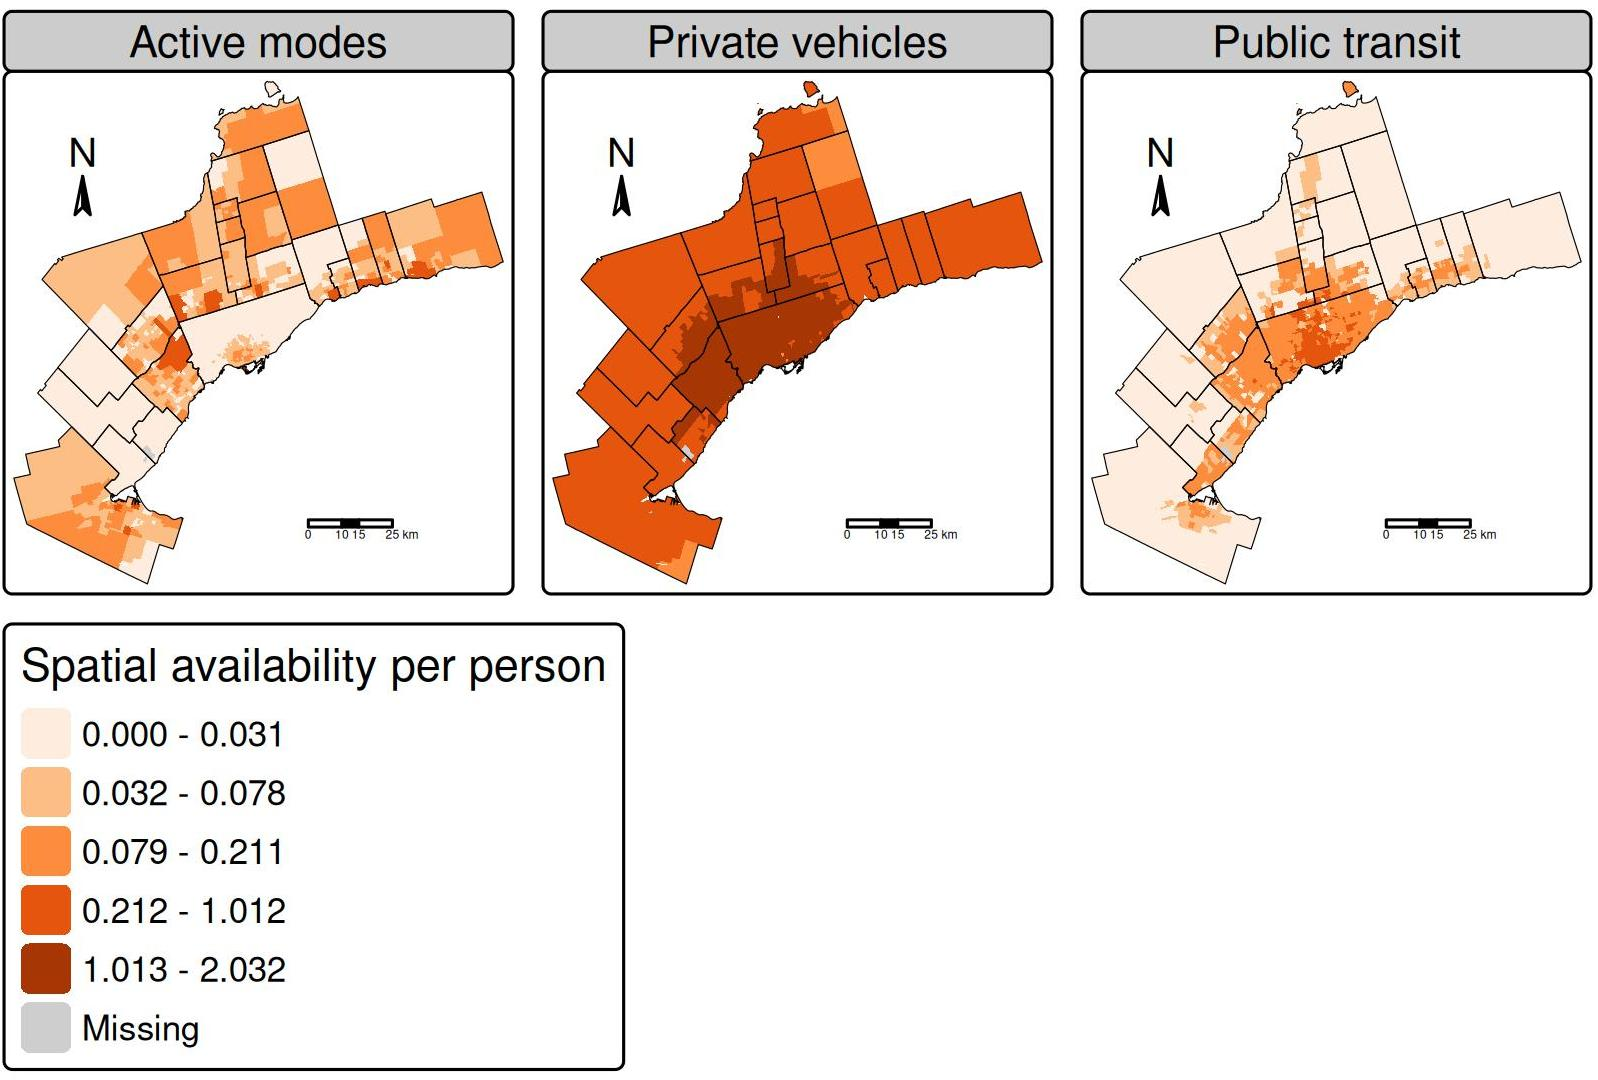
\includegraphics[width=1\linewidth]{figures/SA_pp_3modes_v2_clipped} \caption{Maps of the multimodal spatial availability per person, considering active, public transit and \DIFdelbeginFL \DIFdelFL{motorized modes}\DIFdelendFL \DIFaddbeginFL \DIFaddFL{private vehicles (accessibility values are classified using quintile breaks)}\DIFaddendFL .}\label{fig:multi-sa-pp}
\end{figure}

Transit accessibility appears to be more spatially distributed across
the study area, with the city of Toronto presenting the highest rate of
jobs accessible per transit commuters. Overall, we can observe an
expected spatial pattern where CTs close to public transit
infrastructure present higher levels of transit accessibility when
compared to suburbs and rural areas, which often lack public transit
services.

Next, the map of the active jobs accessible per active traveller
(walkers or cyclists) does not present a clear spatial pattern, with
many suburban and rural areas presenting higher levels when compared to
more urbanized areas. This can be explained by either a higher number of
jobs accessible within typical walking or cycling trip durations, less
probable; or, probably, because the number of active travellers in these
areas is very low, resulting in a higher rate of jobs per person, in a
way that higher accessibility values in these areas may reflect low
competition rather than higher absolute job availability.

Although \DIFdelbegin \DIFdel{motorized }\DIFdelend \DIFaddbegin \DIFadd{private vehicle }\DIFaddend commuters represent about 78\% of the labour
force, they compete for 96\% of the jobs in the study area. Transit
users represent 15\% of the labour force, but they reach only 3.4\% of
the jobs available, while the remaining 0.6\% \DIFdelbegin \DIFdel{percent }\DIFdelend of jobs available are
competed for by the 7\% of active users. On average, each active user
respondent from the NSTP can access 0.06 jobs, while each transit user
can access, on average, 0.14 jobs. \DIFdelbegin \DIFdel{These both }\DIFdelend \DIFaddbegin \DIFadd{Both these }\DIFaddend measures are substantially
lower than the number of jobs that each \DIFdelbegin \DIFdel{motorized }\DIFdelend \DIFaddbegin \DIFadd{private vehicle }\DIFaddend commuter can
reach, which is approximately one job per commuter on average.

\subsection{The effect of calculated accessibility on perceived
accessibility}\label{the-effect-of-calculated-accessibility-on-perceived-accessibility}

Table \ref{tab:models} presents the two probability models linking
calculated \DIFaddbegin \DIFadd{accessibility }\DIFaddend to perceived accessibility \DIFdelbegin \DIFdel{. We }\DIFdelend \DIFaddbegin \DIFadd{and employment
outcome. Based on Wald tests, we }\DIFaddend reject the null hypothesis of weak
instruments and insufficient explanatory power to predict our endogenous
variables (\DIFaddbegin \DIFadd{the }\DIFaddend calculated accessibility indicators)\DIFdelbegin \DIFdel{based on Wald
tests, given that all of the }\DIFdelend \DIFaddbegin \DIFadd{, as all }\DIFaddend F-statistics
are \DIFdelbegin \DIFdel{much higher than }\DIFdelend \DIFaddbegin \DIFadd{well above }\DIFaddend the Stock--Yogo critical values and \DIFdelbegin \DIFdel{are }\DIFdelend statistically
significant (p-value \textless{} 0.05). \DIFdelbegin \DIFdel{However}\DIFdelend \DIFaddbegin \DIFadd{In the categorical models}\DIFaddend , the
first-stage residuals were non-significant in the second-stage
regressions, suggesting \DIFdelbegin \DIFdel{that there
is }\DIFdelend little evidence of endogeneity in the calculated
accessibility indicators, and that standard regressions \DIFdelbegin \DIFdel{(}\DIFdelend without the IV
approach \DIFdelbegin \DIFdel{)
}\DIFdelend could also have been appropriate. \DIFdelbegin \DIFdel{Despite that , we decided to continue
our analysis using the models that account for potential endogeneity}\DIFdelend \DIFaddbegin \DIFadd{However, a Wu-Hausman test on
the linear (continuous) version of the employment-outcome model does
detect endogeneity (p = 0.019; Appendix \ref{tab:iv-diagnostics}),
suggesting that the categorical model's failure to detect it may reflect
a loss of statistical power from quintile-categorization rather than
genuine exogeneity. Given this, we retained the IV framework throughout
our analysis rather than reverting to standard regressions}\DIFaddend .

\begin{table}

\caption{\label{tab:unnamed-chunk-2}\label{tab:models}Weighted ordinal logistic regression models connecting calculated to perceived accessibility \DIFaddbeginFL \DIFaddFL{and to employment outcome}\DIFaddendFL .}
\centering
\DIFdelbeginFL %DIFDELCMD < \begin{tabular}[t]{lcccccc}
%DIFDELCMD < \toprule
%DIFDELCMD < \multicolumn{1}{c}{ } & \multicolumn{3}{c}{\textbf{Few jobs}} & \multicolumn{3}{c}{\textbf{Decline employment}} \\
%DIFDELCMD < \cmidrule(l{3pt}r{3pt}){2-4} \cmidrule(l{3pt}r{3pt}){5-7}
%DIFDELCMD < \textbf{Variable} & \textbf{OR} & \textbf{SE} & \textbf{p-value} & \textbf{OR} & \textbf{SE} & \textbf{p-value}\\
%DIFDELCMD < \midrule
%DIFDELCMD < Active job accessibility per active traveller & \textbf{0.86*} & 0.064 & 0.024 & \textbf{0.84*} & 0.085 & 0.033\\
%DIFDELCMD < Active mode interaction: accessibility × user & \textbf{1.17*} & 0.072 & 0.029 & \textbf{1.21*} & 0.091 & 0.036\\
%DIFDELCMD < Transit job accessibility per transit user & \textbf{1.25*} & 0.112 & 0.044 & 0.89 & 0.191 & 0.5\\
%DIFDELCMD < Transit mode interaction: accessibility × user & 0.95 & 0.133 & 0.7 & 1.16 & 0.208 & 0.5\\
%DIFDELCMD < Motorized job accessibility per motorized user & 0.93 & 0.097 & 0.4 & 1.17 & 0.147 & 0.3\\
%DIFDELCMD < \addlinespace
%DIFDELCMD < Number of Cars & 0.98 & 0.121 & 0.9 & 1.11 & 0.137 & 0.4\\
%DIFDELCMD < Number of Bikes & 1.08 & 0.067 & 0.2 & 1.02 & 0.066 & 0.7\\
%DIFDELCMD < Preferred mode match most frequent mode & 1.14 & 0.168 & 0.4 & 1.27 & 0.246 & 0.3\\
%DIFDELCMD < Montly or annual public transit pass & \textbf{0.68*} & 0.174 & 0.026 & \textbf{0.52*} & 0.257 & 0.012\\
%DIFDELCMD < Public transit availability in the neighbourhood & 0.75 & 0.245 & 0.3 & 1.04 & 0.228 & 0.9\\
%DIFDELCMD < \addlinespace
%DIFDELCMD < Indigenous or racialized person & \textbf{0.60**} & 0.164 & 0.002 & \textbf{0.57**} & 0.211 & 0.008\\
%DIFDELCMD < Temporary visa or refugee & 1.61 & 0.257 & 0.064 & 0.70 & 0.421 & 0.4\\
%DIFDELCMD < Person with disability & 0.69 & 0.209 & 0.077 & 0.80 & 0.232 & 0.3\\
%DIFDELCMD < Woman, transgender or non-binary person & 1.05 & 0.149 & 0.7 & 1.02 & 0.195 & >0.9\\
%DIFDELCMD < Age & 1.01 & 0.006 & 0.080 & \textbf{1.02*} & 0.007 & 0.023\\
%DIFDELCMD < \addlinespace
%DIFDELCMD < Household size & 1.06 & 0.052 & 0.2 & 0.94 & 0.068 & 0.4\\
%DIFDELCMD < Household income &  &  & 0.11 & \textbf{**} &  & 0.004\\
%DIFDELCMD < \hspace{1em}Less than \$40,000 & — & — &  & — & — & \\
%DIFDELCMD < \hspace{1em}\$40,000 to \$80,000 & 0.80 & 0.188 &  & 1.50 & 0.272 & \\
%DIFDELCMD < \hspace{1em}\$80,000 to \$120,000 & 1.23 & 0.220 &  & 1.99 & 0.250 & \\
%DIFDELCMD < \addlinespace
%DIFDELCMD < \hspace{1em}More than \$120,000 & 1.29 & 0.227 &  & 3.08 & 0.314 & \\
%DIFDELCMD < Population density (people/km2) & \textbf{1.18*} & 0.075 & 0.024 & 1.10 & 0.101 & 0.3\\
%DIFDELCMD < Population centre class &  &  & 0.3 & \textbf{***} &  & <0.001\\
%DIFDELCMD < \hspace{1em}Rural & — & — &  & — & — & \\
%DIFDELCMD < \hspace{1em}Small & 1.34 & 0.487 &  & 0.86 & 0.484 & \\
%DIFDELCMD < \addlinespace
%DIFDELCMD < \hspace{1em}Medium & 2.35 & 0.469 &  & 5.13 & 0.457 & \\
%DIFDELCMD < \hspace{1em}Large & 1.25 & 0.322 &  & 1.16 & 0.331 & \\
%DIFDELCMD < Residuals: Active acessibility & 1.09 & 0.078 & 0.3 & 0.97 & 0.085 & 0.7\\
%DIFDELCMD < Residuals: Transit acessibility & 0.85 & 0.092 & 0.073 & 0.85 & 0.148 & 0.3\\
%DIFDELCMD < Residuals: Motorized acessibility & 1.13 & 0.068 & 0.075 & 0.97 & 0.094 & 0.7\\
%DIFDELCMD < \bottomrule
%DIFDELCMD < \multicolumn{7}{l}{\rule{0pt}{1em}Abbreviations: CI = Confidence Interval, OR = Odds Ratio, SE = Standard Error}\\
%DIFDELCMD < \multicolumn{7}{l}{\textsuperscript{} *p<0.05; **p<0.01; ***p<0.001.}\\
%DIFDELCMD < \end{tabular}
%DIFDELCMD < %%%
\DIFdelendFL \DIFaddbeginFL \begin{tabular}[t]{lcccccc}
\toprule
\multicolumn{1}{c}{ } & \multicolumn{3}{c}{\textbf{Few jobs}} & \multicolumn{3}{c}{\textbf{Declined job offers}} \\
\cmidrule(l{3pt}r{3pt}){2-4} \cmidrule(l{3pt}r{3pt}){5-7}
\textbf{Variable} & \textbf{OR} & \textbf{SE} & \textbf{p-value} & \textbf{OR} & \textbf{SE} & \textbf{p-value}\\
\midrule
Active job accessibility per active traveller & \textbf{0.86*} & 0.064 & 0.024 & \textbf{0.84*} & 0.085 & 0.033\\
Active mode interaction: accessibility × user & \textbf{1.17*} & 0.072 & 0.029 & \textbf{1.21*} & 0.091 & 0.036\\
Transit job accessibility per transit user & \textbf{1.25*} & 0.112 & 0.044 & 0.89 & 0.191 & 0.5\\
Transit mode interaction: accessibility × user & 0.95 & 0.133 & 0.7 & 1.16 & 0.208 & 0.5\\
Private vehicle accessibility per user & 0.93 & 0.097 & 0.4 & 1.17 & 0.147 & 0.3\\
\addlinespace
Number of Cars & 0.98 & 0.121 & 0.9 & 1.11 & 0.137 & 0.4\\
Number of Bikes & 1.08 & 0.067 & 0.2 & 1.02 & 0.066 & 0.7\\
Preferred mode match most frequent mode & 1.14 & 0.168 & 0.4 & 1.27 & 0.246 & 0.3\\
Monthly or annual public transit pass & \textbf{0.68*} & 0.174 & 0.026 & \textbf{0.52*} & 0.257 & 0.012\\
Public transit availability in the neighbourhood & 0.75 & 0.245 & 0.3 & 1.04 & 0.228 & 0.9\\
\addlinespace
Indigenous or racialized person & \textbf{0.60**} & 0.164 & 0.002 & \textbf{0.57**} & 0.211 & 0.008\\
Temporary visa or refugee & 1.61 & 0.257 & 0.064 & 0.70 & 0.421 & 0.4\\
Person with disability & 0.69 & 0.209 & 0.077 & 0.80 & 0.232 & 0.3\\
Woman, transgender or non-binary person & 1.05 & 0.149 & 0.7 & 1.02 & 0.195 & >0.9\\
Age & 1.01 & 0.006 & 0.080 & \textbf{1.02*} & 0.007 & 0.023\\
\addlinespace
Household size & 1.06 & 0.052 & 0.2 & 0.94 & 0.068 & 0.4\\
Household income &  &  & 0.11 & \textbf{**} &  & 0.004\\
\hspace{1em}Less than \$40,000 & — & — &  & — & — & \\
\hspace{1em}\$40,000 to \$80,000 & 0.80 & 0.188 &  & 1.50 & 0.272 & \\
\hspace{1em}\$80,000 to \$120,000 & 1.23 & 0.220 &  & 1.99 & 0.250 & \\
\addlinespace
\hspace{1em}More than \$120,000 & 1.29 & 0.227 &  & 3.08 & 0.314 & \\
Population density (people/km2) & \textbf{1.18*} & 0.075 & 0.024 & 1.10 & 0.101 & 0.3\\
Population centre class &  &  & 0.3 & \textbf{***} &  & <0.001\\
\hspace{1em}Rural & — & — &  & — & — & \\
\hspace{1em}Small & 1.34 & 0.487 &  & 0.86 & 0.484 & \\
\addlinespace
\hspace{1em}Medium & 2.35 & 0.469 &  & 5.13 & 0.457 & \\
\hspace{1em}Large & 1.25 & 0.322 &  & 1.16 & 0.331 & \\
Residuals: Active accessibility & 1.09 & 0.078 & 0.3 & 0.97 & 0.085 & 0.7\\
Residuals: Transit accessibility & 0.85 & 0.092 & 0.073 & 0.85 & 0.148 & 0.3\\
Residuals: Private vehicle accessibility & 1.13 & 0.068 & 0.075 & 0.97 & 0.094 & 0.7\\
\midrule\\
\addlinespace
Wald F & 2.86 &  &  & 4.85 &  & \\
p‑value & <0.001 &  &  & <0.001 &  & \\
AIC & 6,829 &  &  & 4,312 &  & \\
\bottomrule
\multicolumn{7}{l}{\rule{0pt}{1em}Abbreviations: CI = Confidence Interval, OR = Odds Ratio, SE = Standard Error}\\
\multicolumn{7}{l}{\textsuperscript{} *p<0.05; **p<0.01; ***p<0.001.}\\
\end{tabular}
\DIFaddendFL \end{table}

Calculated accessibility indicators were partially significant across
the models. \DIFdelbegin \DIFdel{Motorized }\DIFdelend \DIFaddbegin \DIFadd{Private vehicle }\DIFaddend accessibility did not present significant
values for any of the models, probably due to its ubiquity and
homogeneity across the study area.

The model related to the perception of job availability (i.e., ``there
are too few jobs available for me in my ideal commuting time'') \DIFdelbegin \DIFdel{captures
well the expected behaviour of accessibility}\DIFdelend \DIFaddbegin \DIFadd{produces
an estimated association consistent with our hypothesized causal effect}\DIFaddend ,
in which increases in calculated transit and active accessibility \DIFdelbegin \DIFdel{is }\DIFdelend \DIFaddbegin \DIFadd{are
}\DIFaddend associated with a higher probability of having a more positive of
\DIFaddbegin \DIFadd{perception of }\DIFaddend accessibility. In fact, this is the model in which the
\DIFdelbegin \DIFdel{outcome }\DIFdelend \DIFaddbegin \DIFadd{dependent variable }\DIFaddend is the most similar to the spatial availability of
jobs definition, which refers directly to the number of jobs accessible,
calculated using the impedance functions calibrated based on population
behaviour. For this model, one additional job accessible by transit per
transit user increases the average odds of being in a more positive
perception group by 25\%, indicating that fewer respondents agree that
there are too few jobs accessible within their ideal commuting time.
Active accessibility \DIFdelbegin \DIFdel{plays an overall }\DIFdelend \DIFaddbegin \DIFadd{has a negative and }\DIFaddend significant effect for
non-active travellers, reducing the odds of being in a more positive
perception category by 14\%. For active travellers, on the other hand,
the interaction effect more than offsets this to result in a net
positive effect. The same occurs in the model related to \DIFdelbegin \DIFdel{declining
employment}\DIFdelend \DIFaddbegin \DIFadd{declined job
offers due to transport constraints}\DIFaddend , whereby active accessibility is
negative for non-active travellers, but positive for active travellers.
We believe that the general negative effect of active accessibility for
non-active travellers can be explained in terms of job competition,
since increasing the number of jobs accessible for a mode that an
individual does not use implies greater competition for jobs accessible
through other modes, effectively reducing perceived accessibility for
the mode a person actually uses. In addition, as previously shown in
Figure \ref{fig:multi-sa-pp}, many of the areas with high active
accessibility are located outside downtown cores, in more suburban areas
with a low concentration of job opportunities. This \DIFdelbegin \DIFdel{further }\DIFdelend reinforces the
assumption that some suburban areas exhibit high active accessibility
not because of greater job availability, but due to a very low number of
active travellers, resulting in a higher rate of jobs per person -
reflecting low competition for jobs accessible by walking and cycling
rather than higher active job availability.

Table \ref{tab:controls_pop} presents the control variable values
applied for each individual profile, while Figure
\ref{fig:transit-accessibility-thresholds} displays the specific effect
of increasing transit accessibility across the selected individual
profiles for the ``few jobs available'' model. For all of them, we
observe a decrease in negative perceptions as calculated transit
accessibility increases. For the \DIFdelbegin \DIFdel{equity-deserving }\DIFdelend \DIFaddbegin \DIFadd{transport-disadvantaged }\DIFaddend individual
profile, the ``Most negative'' perception has \DIFaddbegin \DIFadd{a }\DIFaddend high probability at low
levels of calculated accessibility. In fact, at the median calculated
transit accessibility (0.12 jobs accessible by public transit per
transit user, calculated based on all NSTP respondents), the two most
negative perception categories (``Most negative'' and ``Negative'')
together account for over 52\% of the total probability, resulting in a
high likelihood that individuals in the \DIFdelbegin \DIFdel{equity-deserving group
to }\DIFdelend \DIFaddbegin \DIFadd{transport-disadvantaged group
will }\DIFaddend have negative perceptions at this accessibility level. For the most
common population, the initial pattern appears similar to the
\DIFdelbegin \DIFdel{equity-deserving
}\DIFdelend \DIFaddbegin \DIFadd{transport-disadvantaged }\DIFaddend group, but the decline in negative perceptions
occurs faster, with the ``Most positive'' probability surpassing
negative probabilities at approximately 0.28 jobs per transit user. In
contrast, for the advantaged population, we can see that even at very
low levels of accessibility, the positive perceptions already present
the highest probabilities and increasing transit accessibility only
reinforces these positive perceptions.

\begin{table}
\centering
\caption{\label{tab:controls}\label{tab:controls_pop}Individual profiles to estimate probabilities.}
\centering
\DIFdelbeginFL %DIFDELCMD < \fontsize{10}{12}\selectfont
%DIFDELCMD < \begin{tabu} %%%
\DIFdelFL{to }%DIFDELCMD < \linewidth {%%%
\DIFdelFL{>}%DIFDELCMD < {\raggedright}%%%
\DIFdelFL{X>}%DIFDELCMD < {\centering}%%%
\DIFdelFL{X>}%DIFDELCMD < {\centering}%%%
\DIFdelFL{X>}%DIFDELCMD < {\centering}%%%
\DIFdelFL{X}%DIFDELCMD < }
%DIFDELCMD < \toprule
%DIFDELCMD < %%%
\DIFdelFL{Variable }%DIFDELCMD < & %%%
\DIFdelFL{Equity-deserving }%DIFDELCMD < & %%%
\DIFdelFL{Most common population }%DIFDELCMD < & %%%
\DIFdelFL{Advantaged group}%DIFDELCMD < \\
%DIFDELCMD < \midrule
%DIFDELCMD < %%%
\DIFdelFL{Number of Cars }%DIFDELCMD < & %%%
\DIFdelFL{0 }%DIFDELCMD < & %%%
\DIFdelFL{1 }%DIFDELCMD < & %%%
\DIFdelFL{2}%DIFDELCMD < \\
%DIFDELCMD < %%%
\DIFdelFL{Number of Bikes }%DIFDELCMD < & %%%
\DIFdelFL{0 }%DIFDELCMD < & %%%
\DIFdelFL{1 }%DIFDELCMD < & %%%
\DIFdelFL{1}%DIFDELCMD < \\
%DIFDELCMD < %%%
\DIFdelFL{Preferred mode match most frequent mode }%DIFDELCMD < & %%%
\DIFdelFL{No }%DIFDELCMD < & %%%
\DIFdelFL{Yes }%DIFDELCMD < & %%%
\DIFdelFL{Yes}%DIFDELCMD < \\
%DIFDELCMD < %%%
\textbf{\DIFdelFL{Indigenous or racialized person}} %DIFAUXCMD
%DIFDELCMD < & %%%
\textbf{\DIFdelFL{Yes}} %DIFAUXCMD
%DIFDELCMD < & %%%
\textbf{\DIFdelFL{Yes}} %DIFAUXCMD
%DIFDELCMD < & %%%
\textbf{\DIFdelFL{No}}%DIFAUXCMD
%DIFDELCMD < \\
%DIFDELCMD < %%%
\DIFdelFL{Temporary visa or refugee }%DIFDELCMD < & %%%
\DIFdelFL{Yes }%DIFDELCMD < & %%%
\DIFdelFL{No }%DIFDELCMD < & %%%
\DIFdelFL{No}%DIFDELCMD < \\
%DIFDELCMD < \addlinespace
%DIFDELCMD < %%%
\DIFdelFL{Person with disability }%DIFDELCMD < & %%%
\DIFdelFL{Yes }%DIFDELCMD < & %%%
\DIFdelFL{No }%DIFDELCMD < & %%%
\DIFdelFL{No}%DIFDELCMD < \\
%DIFDELCMD < %%%
\DIFdelFL{Woman, transgender or non-binary person }%DIFDELCMD < & %%%
\DIFdelFL{Yes }%DIFDELCMD < & %%%
\DIFdelFL{No }%DIFDELCMD < & %%%
\DIFdelFL{No}%DIFDELCMD < \\
%DIFDELCMD < %%%
\textbf{\DIFdelFL{Age}} %DIFAUXCMD
%DIFDELCMD < & %%%
\textbf{\DIFdelFL{35}} %DIFAUXCMD
%DIFDELCMD < & %%%
\textbf{\DIFdelFL{40}} %DIFAUXCMD
%DIFDELCMD < & %%%
\textbf{\DIFdelFL{45}}%DIFAUXCMD
%DIFDELCMD < \\
%DIFDELCMD < %%%
\DIFdelFL{Household size }%DIFDELCMD < & %%%
\DIFdelFL{3 }%DIFDELCMD < & %%%
\DIFdelFL{3 }%DIFDELCMD < & %%%
\DIFdelFL{3}%DIFDELCMD < \\
%DIFDELCMD < %%%
\textbf{\DIFdelFL{Household income}} %DIFAUXCMD
%DIFDELCMD < & %%%
\textbf{\DIFdelFL{Less than \$40,000}} %DIFAUXCMD
%DIFDELCMD < & %%%
\textbf{\DIFdelFL{\$40,000 to \$80,000}} %DIFAUXCMD
%DIFDELCMD < & %%%
\textbf{\DIFdelFL{More than \$120,000}}%DIFAUXCMD
%DIFDELCMD < \\
%DIFDELCMD < \addlinespace
%DIFDELCMD < %%%
\textbf{\DIFdelFL{Population centre class}} %DIFAUXCMD
%DIFDELCMD < & %%%
\textbf{\DIFdelFL{Small}} %DIFAUXCMD
%DIFDELCMD < & %%%
\textbf{\DIFdelFL{Large}} %DIFAUXCMD
%DIFDELCMD < & %%%
\textbf{\DIFdelFL{Large}}%DIFAUXCMD
%DIFDELCMD < \\
%DIFDELCMD < %%%
\DIFdelFL{Public transit availability in the neighbourhood }%DIFDELCMD < & %%%
\DIFdelFL{Yes }%DIFDELCMD < & %%%
\DIFdelFL{Yes }%DIFDELCMD < & %%%
\DIFdelFL{Yes}%DIFDELCMD < \\
%DIFDELCMD < %%%
\textbf{\DIFdelFL{Montly or annual public transit pass}} %DIFAUXCMD
%DIFDELCMD < & %%%
\textbf{\DIFdelFL{Yes}} %DIFAUXCMD
%DIFDELCMD < & %%%
\textbf{\DIFdelFL{No}} %DIFAUXCMD
%DIFDELCMD < & %%%
\textbf{\DIFdelFL{No}}%DIFAUXCMD
%DIFDELCMD < \\
%DIFDELCMD < \bottomrule
%DIFDELCMD < \multicolumn{4}{l}{\textsuperscript{} Bold variables are statistically significant (p-value < 0.05) for at least one of the models.}\\
%DIFDELCMD < \end{tabu}
%DIFDELCMD < %%%
\DIFdelendFL \DIFaddbeginFL \resizebox{\ifdim\width>\linewidth\linewidth\else\width\fi}{!}{
\fontsize{10}{12}\selectfont
\begin{tabular}[t]{lccc}
\toprule
Variable & Transport-disadvantaged & Most common population & Advantaged group\\
\midrule
Number of Cars & 0 & 1 & 2\\
Number of Bikes & 0 & 1 & 1\\
Preferred mode match most frequent mode & No & Yes & Yes\\
\textbf{Indigenous or racialized person} & \textbf{Yes} & \textbf{Yes} & \textbf{No}\\
Temporary visa or refugee & Yes & No & No\\
\addlinespace
Person with disability & Yes & No & No\\
Woman, transgender or non-binary person & Yes & No & No\\
\textbf{Age} & \textbf{35} & \textbf{40} & \textbf{45}\\
Household size & 3 & 3 & 3\\
\textbf{Household income} & \textbf{Less than \$40,000} & \textbf{\$40,000 to \$80,000} & \textbf{More than \$120,000}\\
\addlinespace
\textbf{Population centre class} & \textbf{Small} & \textbf{Large} & \textbf{Large}\\
Public transit availability in the neighbourhood & Yes & Yes & Yes\\
\textbf{Monthly or annual public transit pass} & \textbf{Yes} & \textbf{No} & \textbf{No}\\
\bottomrule
\multicolumn{4}{l}{\textsuperscript{} Bold variables are statistically significant (p-value < 0.05) for at least one of the models.}\\
\end{tabular}}
\DIFaddendFL \end{table}

Regarding the control variables, in the model related to ``there are too
few jobs available for me in my ideal commuting time'', having a monthly
or annual public transit pass is associated with a 32\% reduction in the
odds of being in a more positive category. Being an Indigenous or
racialized person is associated with a reduction of 40\% in the odds of
more positive perceptions, while increasing one person per square
kilometres (population density) was associated with an 18\% increase in
the odds of being in a more positive category.

In the model related to ``I have had to decline employment opportunities
because of my transport situation'', having a monthly or annual public
transit pass reduced the odds of being in a more positive category by
48\%; being Indigenous or racialized reduced the odds by 43\%; and each
additional year of age is associated with an increase of 2\% in the odds
of being in a more positive group. In terms of income, higher income is
associated with more positive perceptions (less perceived employment
decline), with households earning more than \$120,000 CAD having
approximately three times higher odds of being in a positive category
compared to those earning less than \$40,000 CAD. In relation to the
census population centre class, living in a medium-sized population
centre is associated with substantially more positive perceptions (over
five times higher odds), while living in a small centre is associated
with 12\% lower odds, and living in a large centre is associated with
16\% higher odds - all this when compared to rural areas.

\subsection{Equity standards and their impact on tranpostation
equity}\label{equity-standards-and-their-impact-on-tranpostation-equity}

In this section we use the models presented above to identify active
accessibility thresholds, while only the ``there are too few jobs
available for me in my ideal commuting time'' model was selected to
identify \DIFaddbegin \DIFadd{public }\DIFaddend transit thresholds - since \DIFdelbegin \DIFdel{c alculated }\DIFdelend \DIFaddbegin \DIFadd{calculated }\DIFaddend transit
accessibility was statistically significant only in this model.

Figure \ref{fig:transit-accessibility-thresholds} shows the
conservative, intermediate, and progressive public transit thresholds
calculated for each individual profile. For the advantaged profile, a
level of 0 jobs per transit user is already enough to result in positive
perceptions, which means that the current transit accessibility levels
would be sufficient and no individuals would fall below the minimum
accessibility if this profile was selected as the reference. \DIFaddbegin \DIFadd{However, it
is worth noting that this result should not be interpreted as evidence
that public transportation accessibility is irrelevant to the advantaged
group's ability to reach employment. Instead, it demonstrates that the
predicted probability of a positive perception for this profile is
determined primarily by its other characteristics, such as higher
household income and not being a racialized person, so that variation in
accessibility has little additional effect. This is consistent with our
DAG, which shows that individual resources mediate the relationship
between calculated accessibility, perceived accessibility, and
employment outcomes, such that the more advantaged group has a greater
ability to overcome low spatial accessibility through other means.
}\DIFaddend 

\begin{figure}
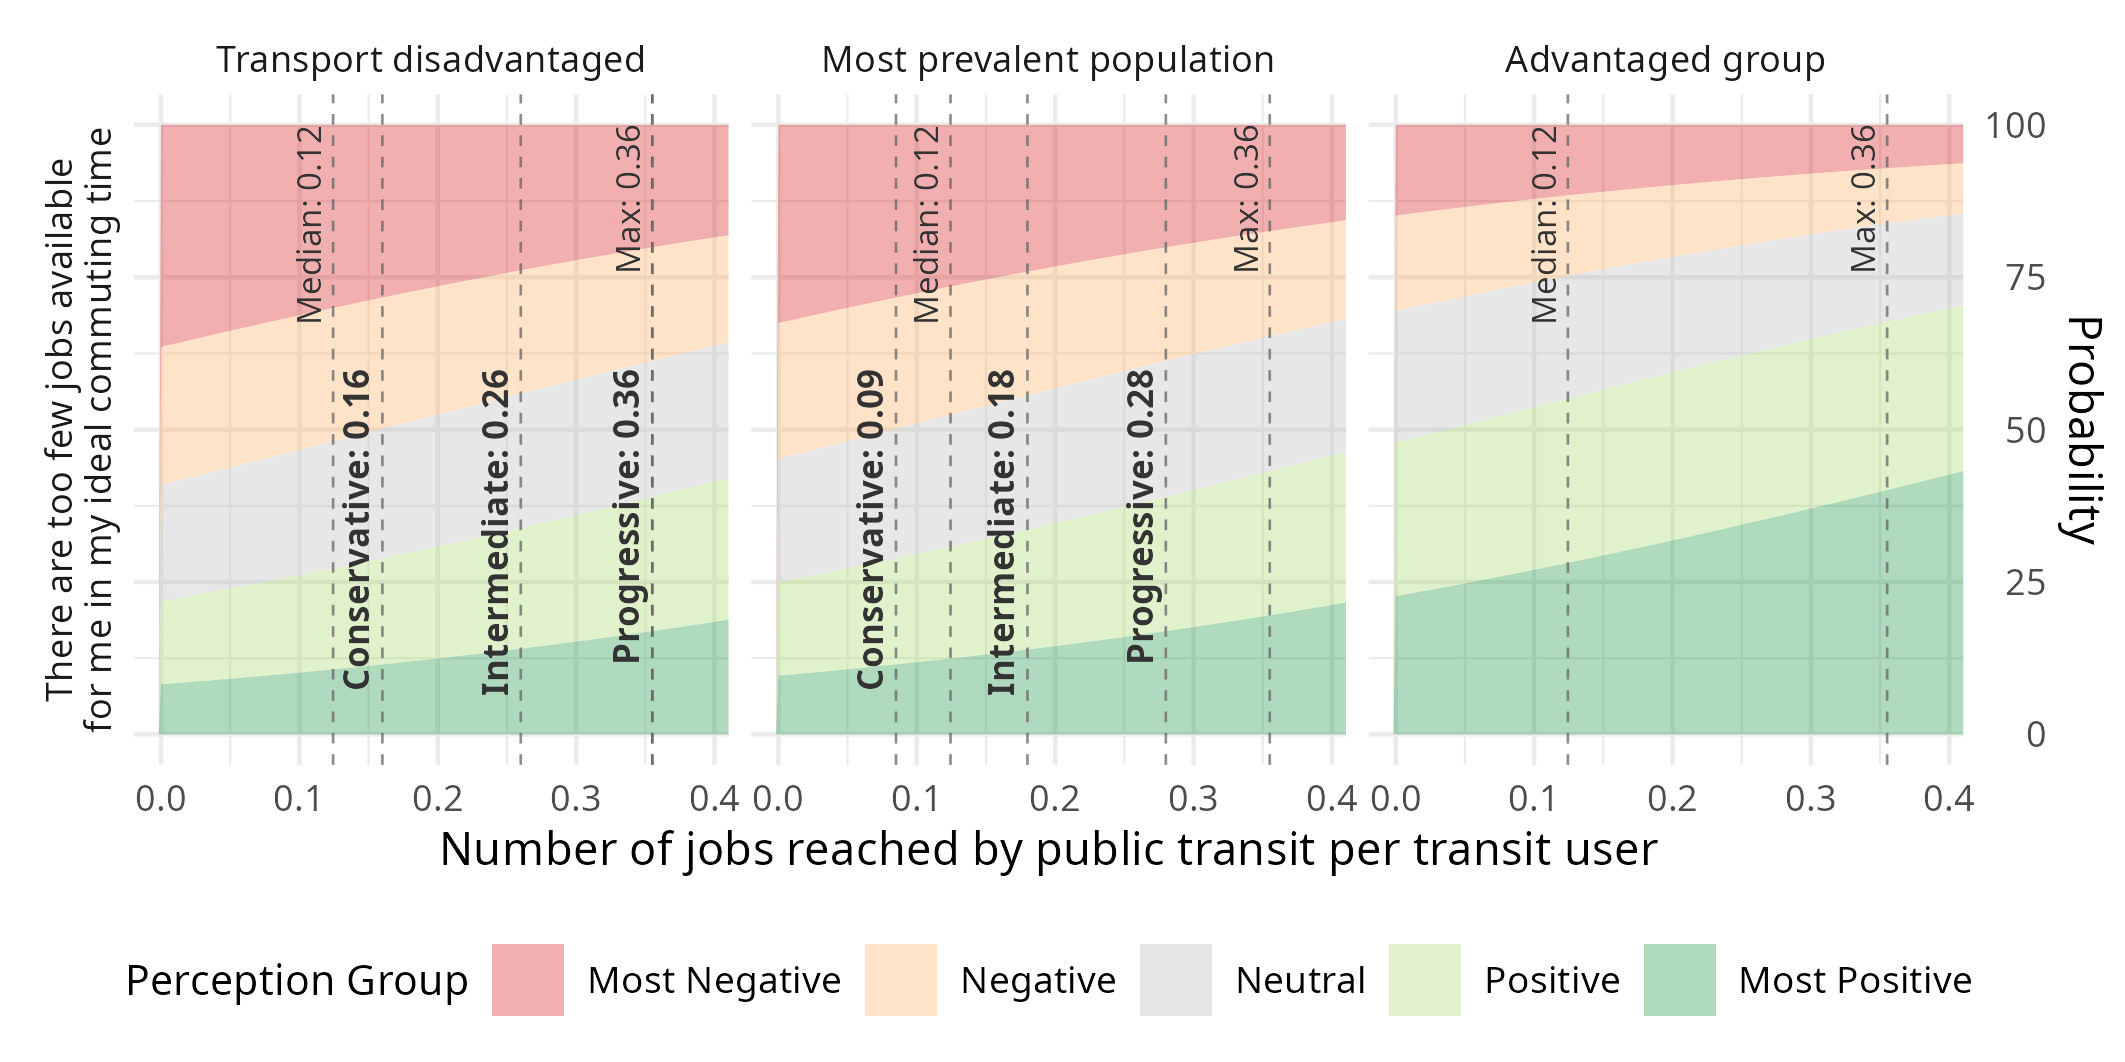
\includegraphics[width=1\linewidth]{figures/accessibility-threshold-v2} \caption{Public transit accessibility thresholds based on selected individual profiles.}\label{fig:transit-accessibility-thresholds}
\end{figure}

For the most common profile, the conservative standard (the minimum
level of accessibility at which the sum of negative perceptions is lower
than the sum of all other perceptions) is equal to 0.09 jobs per transit
user. This threshold is lower than the median calculated transit
accessibility. The progressive threshold, defined as the minimum level
at which the sum of positive perceptions exceeds the sum of negative
perceptions, for this profile is 0.28 jobs per transit user, with the
intermediate threshold defined as the midpoint between these two values
(0.18). However, for the \DIFdelbegin \DIFdel{equity-deserving }\DIFdelend \DIFaddbegin \DIFadd{transport-disadvantaged }\DIFaddend profile, the
conservative threshold is equal to 0.16 jobs per transit user, which is
higher than the median accessibility level. The progressive standard is
equal to 0.36 jobs per transit user, which corresponds to the maximum
observed level of accessibility in the study area, and the intermediate
threshold is 0.26.

Evaluating the thresholds for active accessibility, we again find that
even a minimal level of accessible jobs per active traveller is already
\DIFdelbegin \DIFdel{enough to result in }\DIFdelend \DIFaddbegin \DIFadd{related to }\DIFaddend positive perceptions for the most advantaged profile in both
models\DIFdelbegin \DIFdel{, meaning that the current active accessibility levels
would be sufficient and no individuals would fall below the minimum
accessibility threshold}\DIFdelend . For the most common profile, the identified conservative
threshold is also minimal; and the progressive thresholds are
approximately 1.09 and 2.19 jobs per active user, resulting in higher
probabilities of positive perceptions for the models of \DIFdelbegin \DIFdel{declining
employment }\DIFdelend \DIFaddbegin \DIFadd{declined job
offers }\DIFaddend and few jobs available, respectively.

However, for the model related to \DIFdelbegin \DIFdel{declining employment opportunities }\DIFdelend \DIFaddbegin \DIFadd{declined job offers }\DIFaddend due to
transportation conditions, we were not able to identify a threshold that
resulted in a higher likelihood of positive perceptions for the
\DIFdelbegin \DIFdel{equity-deserving }\DIFdelend \DIFaddbegin \DIFadd{transport-disadvantaged }\DIFaddend profile, even after estimating probabilities at
more than double the maximum observed active accessibility level (2.03
jobs per active user). For the model regarding the perception that there
are too few jobs available within an ideal commuting time, we identified
0.9 as the conservative threshold (22 times the observed median level)
and a progressive threshold close to 5 jobs per active user (almost 2.5
times the maximum observed level and 123 times the median). These high
thresholds are explained by the relatively small net positive effect of
active accessibility, while the other explanatory variables exerted a
greater influence on the estimated probabilities of belonging to a more
positive perception group. Based on both models, the high active
accessibility thresholds help illustrate the limitations of potential
policies focused \DIFdelbegin \DIFdel{solely }\DIFdelend \DIFaddbegin \DIFadd{only }\DIFaddend on increasing active accessibility to promote \DIFdelbegin \DIFdel{positive perceptions}\DIFdelend \DIFaddbegin \DIFadd{a
positive perception and employment outcome}\DIFaddend : an approach that \DIFdelbegin \DIFdel{intervene }\DIFdelend \DIFaddbegin \DIFadd{intervenes
}\DIFaddend only in the spatial dimension of accessibility, without considering the
capacities and travel preferences of the population, would likely result
in limited impact on residents' \DIFdelbegin \DIFdel{perceptions regarding employment reachability and related outcomes}\DIFdelend \DIFaddbegin \DIFadd{perceived accessibility and employment
outcome}\DIFaddend .

\begin{figure}
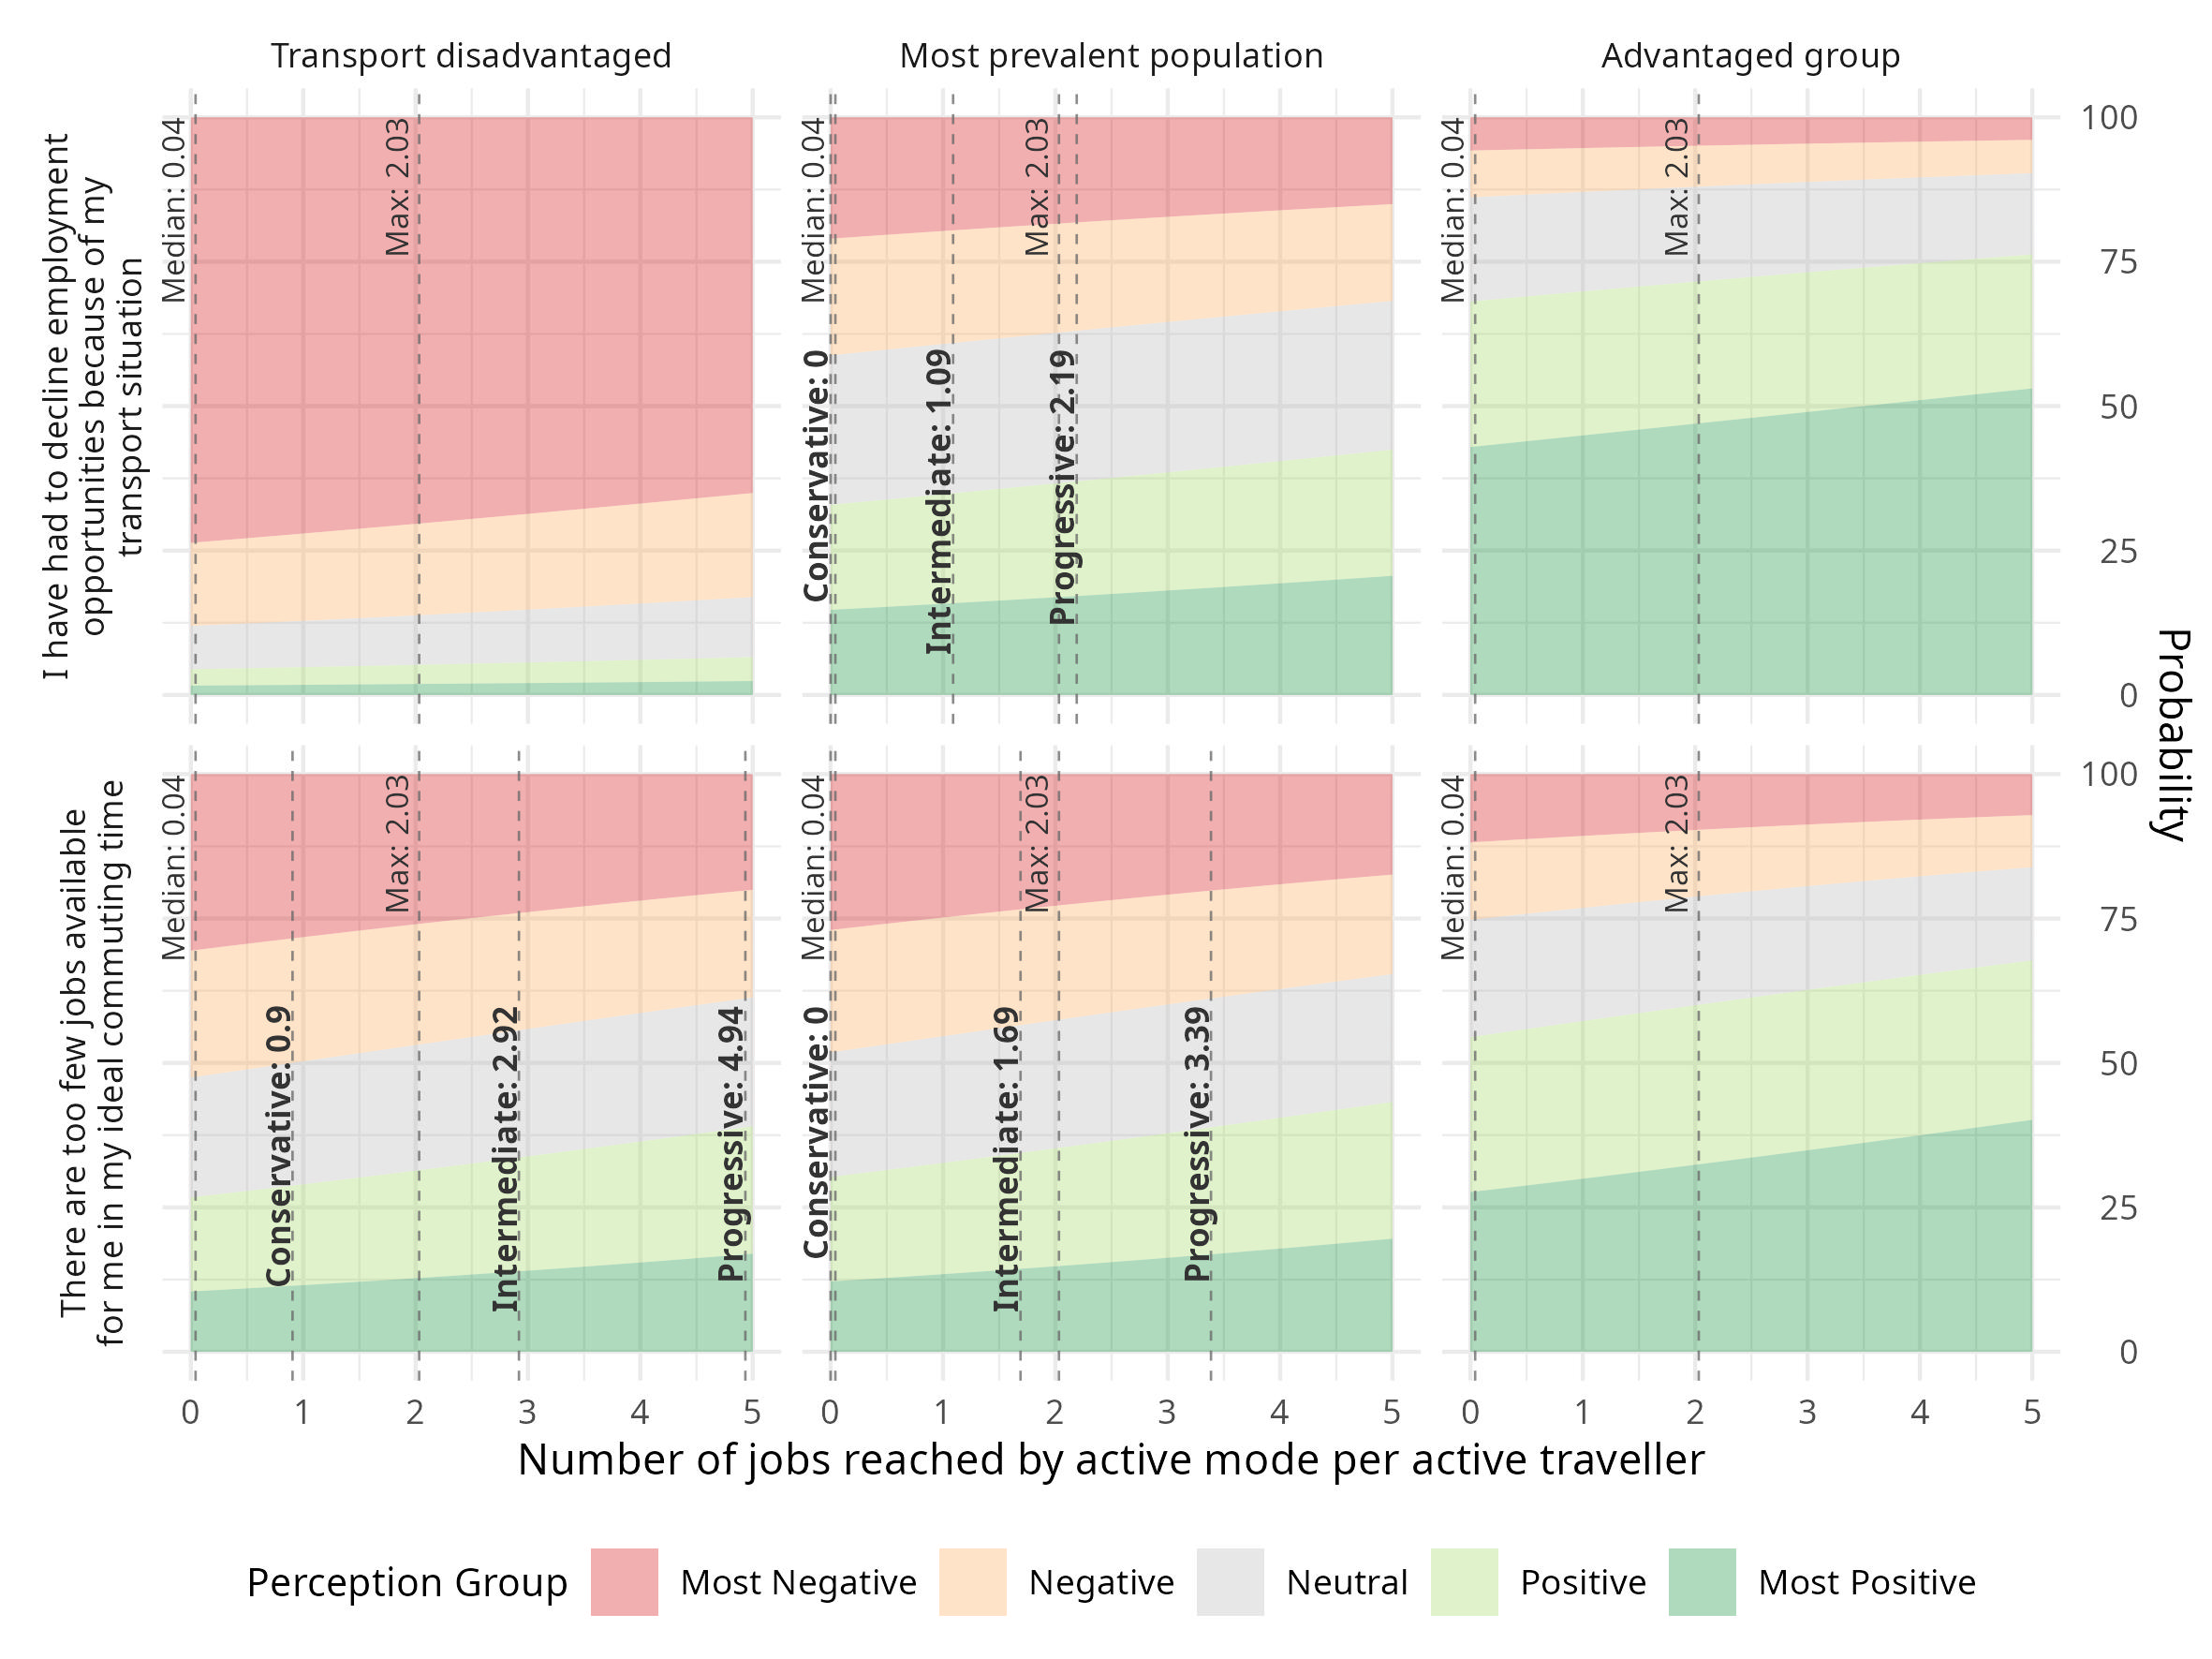
\includegraphics[width=1\linewidth]{figures/accessibility-active-threshold} \caption{Active accessibility thresholds based on selected individual profiles.}\label{fig:active-accessibility-thresholds}
\end{figure}

These thresholds show how, depending on how the socioeconomic and
transportation parameters are controlled and how the individual profiles
are defined, different sufficient levels of accessibility are obtained.
In fact, if one chooses to define thresholds based on the advantaged
profile, it might lead to the conclusion that the current accessibility
state is already sufficient and that no intervention or improvement is
required. Alternatively, \DIFdelbegin \DIFdel{equity-deserving }\DIFdelend \DIFaddbegin \DIFadd{transport-disadvantaged }\DIFaddend groups might still hold
negative perceptions depending on \DIFaddbegin \DIFadd{whether }\DIFaddend the threshold based on the
most common population is selected. Therefore, the only way to ensure
that \DIFdelbegin \DIFdel{equity-deserving }\DIFdelend \DIFaddbegin \DIFadd{transport-disadvantaged }\DIFaddend groups have a better chance of \DIFdelbegin \DIFdel{experience positive perceptions }\DIFdelend \DIFaddbegin \DIFadd{experiencing
positive perceptions and employment outcomes }\DIFaddend is to define minimum
accessibility levels based on the controls tailored to these
populations, setting socioeconomic and transportation parameters that
represent them, thereby adopting a truly equity-based standard.

Considering the feasibility for policy interventions, we suggest the
transit threshold defined in terms of the \DIFdelbegin \DIFdel{equity-deserving profile as examples of equity standards}\DIFdelend \DIFaddbegin \DIFadd{transport-disadvantaged
profile as an example of an equity standard}\DIFaddend . Around 66\% of the study
area population lives in areas with \DIFdelbegin \DIFdel{lower }\DIFdelend transit accessibility levels \DIFaddbegin \DIFadd{lower
}\DIFaddend than the conservative equity standard (0.16), while 91\% live in areas
with transit accessibility levels lower than 0.26 jobs accessible by
transit per transit user (intermediate equity standard), and almost the
entire study area population lives in areas below the progressive equity
standard (0.36, which is also the maximum transit accessibility observed
in the study area). \DIFaddbegin \DIFadd{Regarding the low-income population, 55\% live in
areas with an accessibility gap under the conservative standard, 86\%
under the intermediate standard, and almost all live in areas with an
accessibility gap under the most progressive standard.
}

\DIFaddend In terms of the severity of transport disadvantage (FGT-1), the average
\DIFdelbegin \DIFdel{shortfall }\DIFdelend \DIFaddbegin \DIFadd{gap }\DIFaddend among deprived individuals amounts to 36\% under the conservative
standard, meaning that those who do not meet the threshold fall short of
it by roughly one-third on average (about 0.06). For the \DIFaddbegin \DIFadd{low-income
population, the average shortfall is around 27\% (about 0.04). For the
}\DIFaddend intermediate standard, the average \DIFdelbegin \DIFdel{gap }\DIFdelend \DIFaddbegin \DIFadd{shortfall for the general population
}\DIFaddend is 53\% (about 0.14)\DIFaddbegin \DIFadd{, while it is 44\% (0.11) for the low-income group}\DIFaddend .
For the progressive equity standard, the average shortfall \DIFaddbegin \DIFadd{for the
general population }\DIFaddend is about 0.23 (65\% of the standard)\DIFaddbegin \DIFadd{, and about 0.20
(58\%) for the low-income group}\DIFaddend . These FGT measures show that, as the
minimum transit accessibility levels become more demanding when moving
from conservative to progressive standards, not only \DIFaddbegin \DIFadd{do }\DIFaddend more individuals
fall below the threshold, but those in accessibility \DIFdelbegin \DIFdel{shortfall }\DIFdelend \DIFaddbegin \DIFadd{gap }\DIFaddend are, on
average, substantially further from achieving it. \DIFaddbegin \DIFadd{They also show that
the low-income population is, in general, located in areas with greater
public transportation accessibility than the general population, meaning
that low-income individuals who fall below a certain threshold are, on
average, closer to reaching it and would need comparatively smaller
improvements in accessibility to reach it.
}\DIFaddend 

\subsection{Areas for priority
intervention}\label{areas-for-priority-intervention-1}

Figure \ref{fig:priority_areas} shows the priority areas for policy
intervention for CTs with transit accessibility \DIFdelbegin \DIFdel{shortfall}\DIFdelend \DIFaddbegin \DIFadd{gap for each standard
type}\DIFaddend , based on their \DIFdelbegin \DIFdel{AFI index and for each equity standard type}\DIFdelend \DIFaddbegin \DIFadd{equity-weighted AFI}\DIFaddend . All census subdivisions
contain CTs experiencing transit accessibility \DIFdelbegin \DIFdel{shortfall}\DIFdelend \DIFaddbegin \DIFadd{gap}\DIFaddend , independently of the
type of standard. For the conservative standard, \DIFdelbegin \DIFdel{about 32}\DIFdelend \DIFaddbegin \DIFadd{only 35}\DIFaddend \% of the CTs
(\DIFdelbegin \DIFdel{431 }\DIFdelend \DIFaddbegin \DIFadd{516 }\DIFaddend out of the 1,489 CTs in the study area) present transit
accessibility levels above the shortfall limit, with most of them (\DIFdelbegin \DIFdel{91}\DIFdelend \DIFaddbegin \DIFadd{83}\DIFaddend \%)
located in the City of Toronto. This share of CTs \DIFaddbegin \DIFadd{without an
accessibility gap }\DIFaddend decreases to less than 10\% for the intermediate
equity standard (136 CTs). Only one CT\DIFaddbegin \DIFadd{, }\DIFaddend located in Toronto\DIFaddbegin \DIFadd{, }\DIFaddend does not
present an accessibility \DIFdelbegin \DIFdel{deficit }\DIFdelend \DIFaddbegin \DIFadd{gap }\DIFaddend when evaluated under the progressive
standard. \DIFdelbegin \DIFdel{The unique CT without accessibility shortfall }\DIFdelend \DIFaddbegin \DIFadd{This unique CT }\DIFaddend corresponds to the area surrounding the St\DIFaddbegin \DIFadd{.
}\DIFaddend George Subway Station in Downtown Toronto, \DIFdelbegin \DIFdel{with a connection }\DIFdelend \DIFaddbegin \DIFadd{connected }\DIFaddend to the two subway
lines that cross the city and \DIFdelbegin \DIFdel{connect }\DIFdelend \DIFaddbegin \DIFadd{link }\DIFaddend neighbouring municipalities, running
from \DIFdelbegin \DIFdel{North to South and from East to West. In
addition, this }\DIFdelend \DIFaddbegin \DIFadd{north to south and from east to west. This }\DIFaddend CT is bounded by Spadina
Avenue \DIFdelbegin \DIFdel{on }\DIFdelend \DIFaddbegin \DIFadd{to }\DIFaddend the west and Bloor Street \DIFdelbegin \DIFdel{on }\DIFdelend \DIFaddbegin \DIFadd{to }\DIFaddend the south, with many connections
to the public transit system, including a streetcar line on Spadina.

In terms of areas for policy intervention, \DIFdelbegin \DIFdel{considering }\DIFdelend \DIFaddbegin \DIFadd{by }\DIFaddend the conservative standard,
\DIFdelbegin \DIFdel{the subdivision of Brampton is the one with the largest }\DIFdelend \DIFaddbegin \DIFadd{Hamilton has both the largest low-income }\DIFaddend population living in \DIFdelbegin \DIFdel{areas classified as very
high priority (217,253
people, representing 33}\DIFdelend \DIFaddbegin \DIFadd{very
high-priority areas (44,170 people) and the highest proportion of its
low-income population impacted (73\%, or 8}\DIFaddend \% of the \DIFdelbegin \DIFdel{subdivision population}\DIFdelend \DIFaddbegin \DIFadd{city's residents}\DIFaddend ),
followed by \DIFdelbegin \DIFdel{Hamilton with 184,991 people(32}\DIFdelend \DIFaddbegin \DIFadd{Toronto (23,295 people, although they represent only 6}\DIFaddend \% of
its \DIFdelbegin \DIFdel{residents), Vaughan (144,670
people, 44}\DIFdelend \DIFaddbegin \DIFadd{low-income population and less than 1\% of the city's residents) and
Brampton (13,315 people, 32\% of its low-income population and 2\% of
the city's residents). Considering only the proportion of the low-income
population, Milton (63}\DIFaddend \%) and \DIFdelbegin \DIFdel{Markham (142, 066 people, 41\%).
For the most
}\DIFdelend \DIFaddbegin \DIFadd{Oshawa (55\%) also stand out, despite
their smaller absolute numbers (4,880 and 9,835 people, respectively).
}

\DIFadd{According to the }\DIFaddend progressive standard, \DIFdelbegin \DIFdel{Brampton }\DIFdelend \DIFaddbegin \DIFadd{Toronto }\DIFaddend and Hamilton again \DIFdelbegin \DIFdel{appear having the largest populations living in very high priority }\DIFdelend \DIFaddbegin \DIFadd{have
the largest low-income populations in very high-priority }\DIFaddend areas, with
\DIFdelbegin \DIFdel{380,289
people (}\DIFdelend \DIFaddbegin \DIFadd{about }\DIFaddend 57\% \DIFdelbegin \DIFdel{) and 229,549 people (40\%) respectively, but now followed by the City of Toronto with 221,768 people (7\%).
}%DIFDELCMD < 

%DIFDELCMD < %%%
\DIFdel{However, in terms of population share, 100\% of the populationliving in
the subdivisions of East Gwillimbury (34,637 people), Uxbridge (21,556
people}\DIFdelend \DIFaddbegin \DIFadd{of each subdivision's low-income population living in areas
with accessibility gap, followed by Mississauga, with just over 31,000
low-income people (47\% of its low-income population}\DIFaddend ), and \DIFdelbegin \DIFdel{Whitchurch-Stouffville (49,864 people)are in areas with
very high priority for policy intervention for the conservative and
intermediate standards. For the progressive standard, only
Whitchurch-Stouffville has all its CTs classified as very high priority
areas}\DIFdelend \DIFaddbegin \DIFadd{Richmond Hill
(39\%)}\DIFaddend . This difference occurs because the priority areas are defined
based on their \DIFaddbegin \DIFadd{equity-weighted }\DIFaddend AFI position in the quantile
classification for the entire study area, and as additional CTs are
included under more rigorous standards, the AFI distribution also
\DIFdelbegin \DIFdel{shifts. Regarding the
Whitchurch-Stouffville, this subdivision is served by only one fixed
public transit line managed by GO Transit, a regional train line that
connects Stouffville with the subdivisions of Markham and Toronto. The
list with }\DIFdelend \DIFaddbegin \DIFadd{changes. A list of }\DIFaddend the total number of \DIFaddbegin \DIFadd{low-income }\DIFaddend people living in each
priority area, by equity standard \DIFdelbegin \DIFdel{type }\DIFdelend and subdivision, is available as
supplementary material.

\begin{figure}
\DIFdelbeginFL %DIFDELCMD < 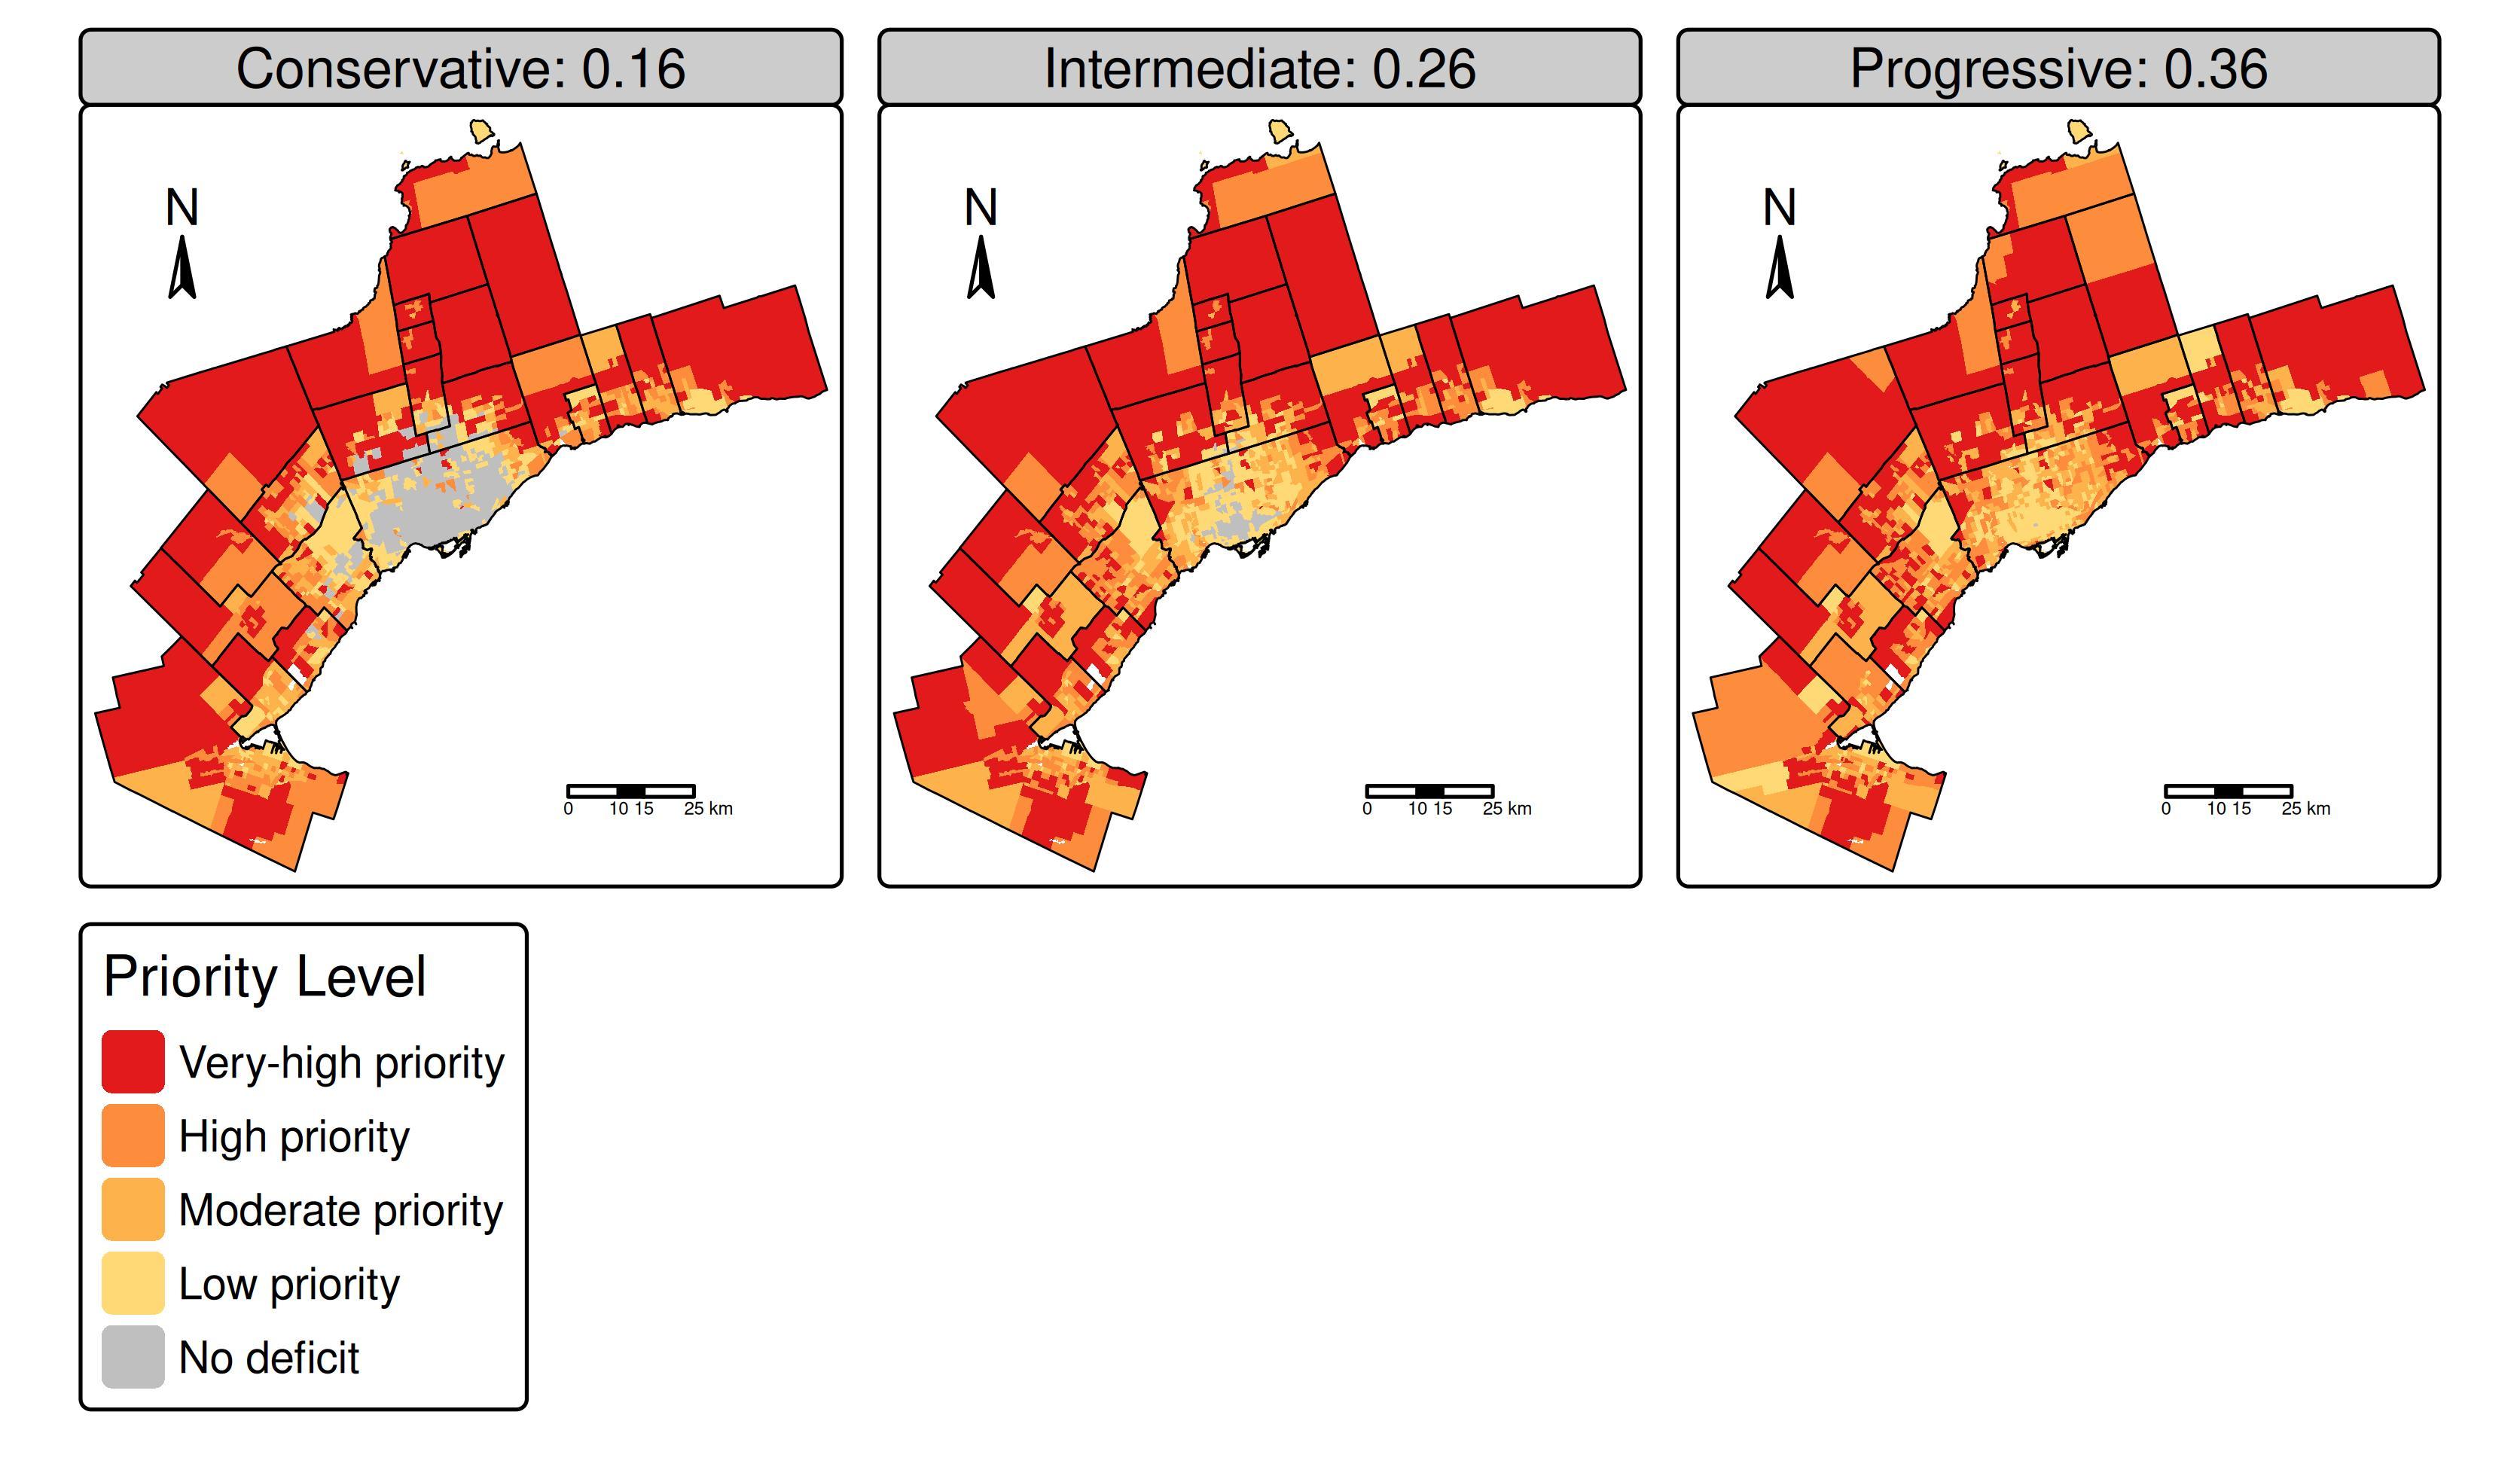
\includegraphics[width=1\linewidth]{figures/geographical_priorities} %%%
\DIFdelendFL \DIFaddbeginFL 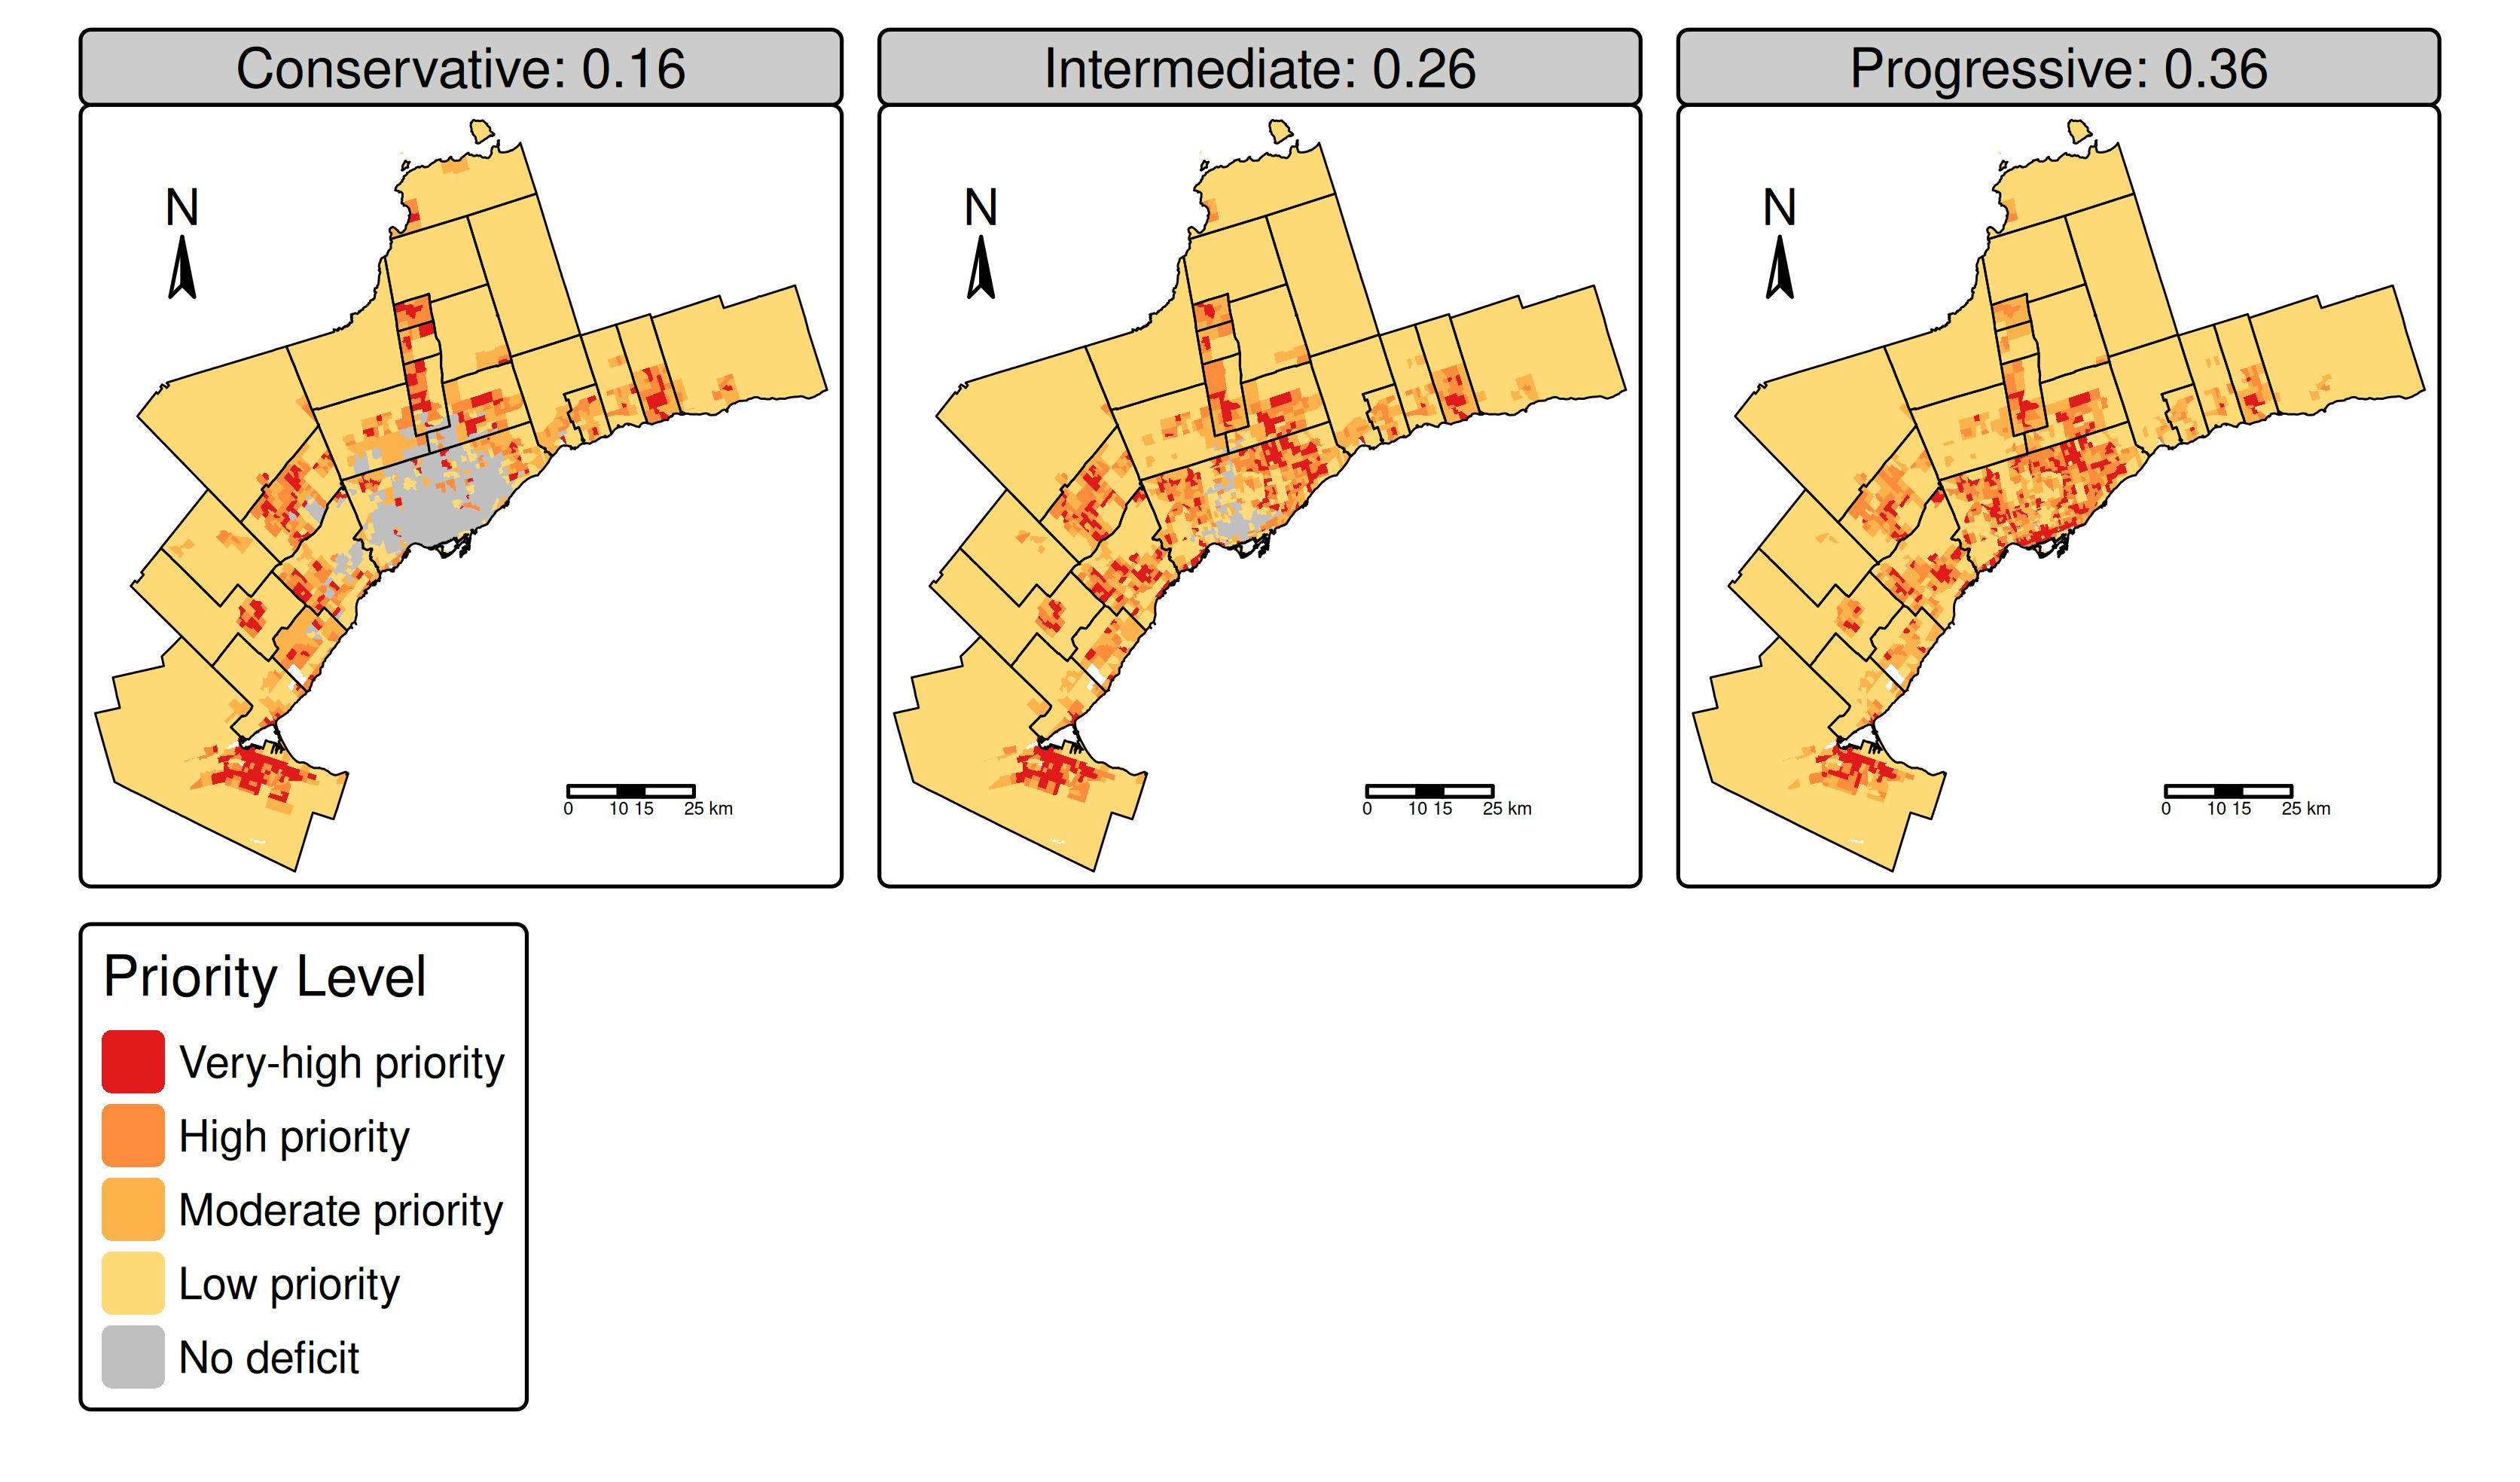
\includegraphics[width=1\linewidth]{figures/geographical_priorities_LIMAT} \DIFaddendFL \caption{Priority areas for policy intervention by type of equity standard.}\label{fig:priority_areas}
\end{figure}

\DIFaddbegin \DIFadd{We believe that the identified priority areas can help guide future
investments in public transportation services and infrastructure. If we
base prioritization only on the amount, share, and size of the
low-income population living in areas with an accessibility gap,
Hamilton and Toronto should potentially be prioritized in order to
provide a more equitable distribution of transportation benefits. It is
worth noting that the City of Hamilton is currently implementing its
first Light Rail Transit (LRT) line in Downtown Hamilton, connecting the
eastern and western parts of the city while also crossing Downtown, an
area that concentrates a large share of the city's available jobs.
Provided the city mitigates potential displacement and relocation of its
low-income population resulting from land price increases associated
with the LRT, its inclusion is likely to have a significant impact on
transportation equity, since the LRT crosses the areas classified as
high priority for policy intervention and with the largest concentration
of low-income residents in the city.
}

\DIFaddend \section{Critical analysis and
limitations}\label{critical-analysis-and-limitations}

\DIFdelbegin \DIFdel{Although the }\DIFdelend \DIFaddbegin \DIFadd{In this study, we present a methodology for defining equity standards
for transportation planning, theoretically guided by the recognition of
accessibility as a human capability, aligned with a sufficientarian and
egalitarian perspective on how it should be distributed. Making explicit
the moral foundations that support our analysis is, in our view,
important because different theories of justice lead to different
perspectives on how policies should manage the distribution of
transport-related benefits. In addition to a theoretical foundation,
equity standards based on accessibility are also operationalized through
the use of thresholds. We propose defining thresholds based on the
estimated relationship between calculated accessibility and perceived
accessibility and employment outcome, and we believe that this approach
is our most significant contribution to transportation studies, and more
specifically to the equitable distribution of transportation benefits,
as it makes these standards easier to communicate with policy
practitioners and the general public. Although the study does not ensure
full reproducibility, since the surveys used are confidential, it does
ensure replicability by making all code available for consultation.
}

\DIFadd{We selected job accessibility as our indicator to define equity
standards for a few reasons. First, employment accessibility is widely
recognized as a key indicator of how well a city or region serves its
residents \mbox{%DIFAUXCMD
\citep{bania2008, owen2015, shen1998}}\hskip0pt%DIFAUXCMD
, and as an indicator of
the ``quality of urban living'' \mbox{%DIFAUXCMD
\citep{wachs1973, handy2020}}\hskip0pt%DIFAUXCMD
, since
employment provides the financial ability to support other life
activities \mbox{%DIFAUXCMD
\citep{merlin2017}}\hskip0pt%DIFAUXCMD
. Second, calculating accessibility
requires the use of impedance functions, and we decided to use
calibrated functions based on empirical data to better represent
people's travel behaviour. Accessibility measures also require land-use
data on both population (for competitive measures) and the number of
opportunities. Both requirements are met by Census microdata
specifically for employment and the labour force, which is not the case
for other types of opportunity. Third, the NSTP survey includes
questions on perceived job accessibility and employment outcomes
specifically, which directly enabled our approach of linking calculated
job accessibility to individuals' perceptions and outcomes related to
this opportunity type. We believe, however, that our methodology can be
extended to other opportunity types essential for a meaningful life,
such as healthcare and education, provided that the analyst has the
necessary data on hand to perform the analysis.
}

\DIFadd{Although the NSTP provides an }\DIFaddend unprecedented look at transport poverty in
Canada\DIFdelbegin \DIFdel{provided
by the NSTP}\DIFdelend , the survey does not contain a question in which the respondent
answers objectively whether they are satisfied or not with their
mobility experiences or overall transport conditions. \DIFdelbegin \DIFdel{Rather}\DIFdelend \DIFaddbegin \DIFadd{More specifically}\DIFaddend ,
the respondents use a continuum scale to answer their level of agreement
with specific statements. The absence of a categorical or binary
variable referring to satisfaction level led us to categorize the
\DIFdelbegin \DIFdel{outcomes}\DIFdelend \DIFaddbegin \DIFadd{outcome}\DIFaddend , in order to identify which perception category the respondent
belongs to, varying from most negative to most positive. In fact, with
the information we have, we cannot infer if the person is satisfied or
not, but rather whether they are more or less satisfied in comparison to
others. The underlying rationale for our standards proposition is to
identify the calculated accessibility level that places the most
disadvantaged population group within the most positive perception
group.

It is worth mentioning that other outcome categorizations or numbers of
categories are possible. For instance, one might decide to convert the
continuum scale to a Likert scale based on fixed intervals, classifying
those with agreement levels \DIFdelbegin \DIFdel{between }\DIFdelend \DIFaddbegin \DIFadd{from }\DIFaddend 0 to 20\%\DIFdelbegin \DIFdel{as ``Most Negative''}\DIFdelend , 20 to 40\%\DIFdelbegin \DIFdel{as ``Negative''}\DIFdelend , and so on, in
pre-determined intervals. The problem with \DIFdelbegin \DIFdel{this }\DIFdelend \DIFaddbegin \DIFadd{the fixed-interval }\DIFaddend approach
is that \DIFdelbegin \DIFdel{, when doing this, }\DIFdelend the analyst is normatively defining levels of satisfaction for
\DIFdelbegin \DIFdel{the }\DIFdelend respondents that might not \DIFdelbegin \DIFdel{represent the actual feeling of the person}\DIFdelend \DIFaddbegin \DIFadd{reflect their actual feelings}\DIFaddend . Because of
this, we decided to categorize responses based on the perception scale
distribution and use the sample population to evaluate those who are
more and less satisfied.

\DIFdelbegin \DIFdel{This outcome }\DIFdelend \DIFaddbegin \DIFadd{To test the sensitivity of our results to the choice of categorization
type, we re-estimated the perception model using a fixed-interval
categorization that does not depend on the sample's distribution,
instead of a quintile-based categorization (classifying responses from 0
to 20 as most positive, 20 to 40 as positive, 40 to 60 as neutral, 60 to
80 as negative, and 80 to 100 as most negative). The results of this
alternative model (Appendix \ref{tab:few_jobs_break_model}) are
consistent with those of the model created using the quintile
classification, with all coefficients that were statistically
significant in the quintile model remaining significant in this
alternative categorization, with matching signs and similar magnitudes
(e.g., transit accessibility: \(\beta = 0.227\), \(p = 0.044\), compared
to \(\beta = 0.223\), \(p = 0.044\) in our main specification; and
active accessibility: \(\beta = -0.145\), \(p = 0.024\), compared to
\(\beta = -0.151\), \(p = 0.024\)), suggesting that our findings are not
an artifact of the specific method used to categorize our dependent
variable.
}

\DIFadd{However, the quintile-based }\DIFaddend categorization caused, in general, the
control variables to lose part of their predictive power when compared
to linear regression models created using the previous continuous forms.
As shown in Table \ref{tab:linear_models}, in general, \DIFdelbegin \DIFdel{the accessibility variables
presented a similar behaviour when compared }\DIFdelend \DIFaddbegin \DIFadd{and similarly }\DIFaddend to
the categorical models\DIFdelbegin \DIFdel{;
However}\DIFdelend \DIFaddbegin \DIFadd{, the accessibility estimates are consistent with
our hypothesized causal effect. In contrast}\DIFaddend , the control variables
presented a better performance in explaining the outcomes in the linear
regressions, such as in the case of the disability indicator and the
``temporary visa or refugee'' variable, which did not present
statistical significance in the categorical version of \DIFdelbegin \DIFdel{the modelfor ``there are too few jobs available
for me in my ideal commuting time.
'' We decided to use the categorical
models because they enabled us to identify levels of satisfaction in
a
non-normative way}\DIFdelend \DIFaddbegin \DIFadd{perception model.
}

\DIFadd{An additional limitation concerns the interpretation of our ``job offer
declined'' indicator. Agreeing or disagreeing with this question
presupposes that the respondent had looked for a job and subsequently
received a job offer that they declined. In this sense, individuals who
did not look for work (including those who may have given up searching
because they anticipated that available jobs would be inaccessible due
to their transportation situation) would not be recorded as having
declined an offer, regardless of the extent to which transportation
constraints limit their employment prospects. This mechanism is
conceptually related to the discussion of adaptive preferences: just as
some people may adjust downward their perceptions of job scarcity in
response to low accessibility, others may give up on the job search
completely. Consequently, the indicator of declined job offers likely
captures transportation-related employment disadvantage only among those
who remain active in the labor market and may underestimate the
prevalence of transportation disadvantage among those most severely
excluded from employment opportunities. We cannot assess this selection
directly using the current cross-sectional data from the NSTP, which do
not allow us to distinguish those who are not looking for work from
those who are actively seeking employment but have not received offers
to decline}\DIFaddend .

Regarding the relationship between perceived and calculated
accessibility, \DIFdelbegin \DIFdel{only transit accessibility , in one of the models,
presented the behaviour hypothesized in }\DIFdelend \DIFaddbegin \DIFadd{the transit accessibility indicator was the most
consistent with our hypothesized causal effect in the perception-based
model, through }\DIFaddend which increasing accessibility was associated with more
positive perceptions. Although the active accessibility indicator
presented a slightly positive net effect for active travellers in both
models, this effect was not sufficient to outweigh the influence of the
other explanatory variables. As a result, the estimated active
thresholds were excessively demanding and unrealistic from a policy
perspective. For one model, we were unable to identify thresholds, while
for the other, the conservative threshold was 22 times higher than the
median accessibility level\DIFaddbegin \DIFadd{, }\DIFaddend and the progressive threshold was more than
123 times higher than the median accessibility \DIFaddbegin \DIFadd{level}\DIFaddend . These results led
us to propose equity standards\DIFdelbegin \DIFdel{based solely on the
model ``there are too few jobs available for me in my ideal commuting
time,'' }\DIFdelend \DIFaddbegin \DIFadd{, exclusively, based on the
perception-based model }\DIFaddend and for public transit mode.

\DIFaddbegin \DIFadd{Additionally, the non-significant residuals in the categorical models
indicate weak evidence of endogeneity in the calculated accessibility
indicators. However, a Wu-Hausman test on the linear (continuous)
version of the employment-outcome model did detect significant
endogeneity (p = 0.019; Appendix \ref{tab:iv-diagnostics}), suggesting
that the categorical models' failure to detect it may instead reflect a
loss of statistical power from quintile-categorization of the dependent
variables. This result reinforces our view that the accessibility
variables are unlikely to be entirely exogenous to the perceived
accessibility indicators and the outcomes analyzed, and that the
instrumental variable framework remains necessary. As is generally the
case in instrumental variable designs
\mbox{%DIFAUXCMD
\citep{cunningham2021causal, huntington-klein2021}}\hskip0pt%DIFAUXCMD
, our assumption that
the instruments affect perceived accessibility and employment outcome
only through calculated accessibility cannot be directly tested. Even
so, adopting an instrumental variable approach was the most suitable
alternative for accounting for potential endogeneity given the use of
cross-sectional surveys.
}

\DIFadd{Our instrumental variable strategy was not specifically designed to
address residential self-selection, and although it offers a degree of
protection against confounding factors more broadly, we cannot exclude
the possibility that unobserved commuting preferences and constraints
that determine residential location choices are correlated with our
spatial filter instruments. A more definitive test would require
longitudinal data tracking individuals across their residential moves
over the years, or an instrument based on a source of variation known to
be exogenous to residential choice; neither of these options is
available in the current cross-sectional NSTP data, nor in the Canadian
Census.
}

\DIFaddend For future research, we suggest exploring additional place-based
accessibility measures to further evaluate the relationship between
calculated and perceived accessibility. For instance, the raw multimodal
spatial availability indicator could be tested. This indicator \DIFdelbegin \DIFdel{uses as
output }\DIFdelend \DIFaddbegin \DIFadd{reflects
}\DIFaddend the number of jobs accessible by \DIFdelbegin \DIFdel{different transport modes, not
standardized }\DIFdelend \DIFaddbegin \DIFadd{each transport mode, without
standardizing }\DIFaddend by the number of people \DIFdelbegin \DIFdel{using these modes}\DIFdelend \DIFaddbegin \DIFadd{competing for those jobs}\DIFaddend . We
decided to use multimodal spatial availability per person because we
believe that competition matters when evaluating perceptions related to
employment outcomes, as demonstrated by previous studies
\citep{jin2018, merlin2017, miller2005}\DIFdelbegin \DIFdel{. Another limiting factor that
led us to adopt the CT level was that we could not estimate travel times
at the DA level for the entire study area due to the memory limitations
of our computational resources. Despite that, the initial tests
performed with a smaller study area did not show differences in terms of
the sign and statistical significance of the accessibility coefficients
between regressions - probably because the indicators are standardized
}\DIFdelend \DIFaddbegin \DIFadd{; and because the standardized
version allows for comparisons across cities with different labour force
and job opportunity sizes}\DIFaddend .

\DIFdelbegin \DIFdel{Continuing with }\DIFdelend \DIFaddbegin \DIFadd{Regarding }\DIFaddend the spatial unit used, the CTs, we recognize that this unit is
not the most detailed among census geographies, being less detailed than
dissemination areas or dissemination blocks. We decided to use CTs due
to the large size of the study area, in order to provide a regional
analysis rather than focus on only one city, considering this entire
basin to calculate the accessibility indicators and select the sample.
This choice is motivated by the recognition of commuting flows across
municipalities, \DIFdelbegin \DIFdel{which are even }\DIFdelend \DIFaddbegin \DIFadd{a pattern that is itself }\DIFaddend one of the parameters used by
Statistics Canada when defining Census Metropolitan Areas. \DIFdelbegin %DIFDELCMD < 

%DIFDELCMD < %%%
\DIFdel{Regarding the equity standards definitions, three moral principles
guided our approach. The first relies on the recognition of
accessibility as a human capability
\mbox{%DIFAUXCMD
\citep{sen2005, sen1999, pereira2017, luz2022}}\hskip0pt%DIFAUXCMD
, something required for a
dignified life \mbox{%DIFAUXCMD
\citep{karner2020}}\hskip0pt%DIFAUXCMD
, and the main transportation benefit
to be distributed across society in order to increase people's freedom.
The second is grounded in the sufficientarian perspective, considering a
fair transportation and land-use system as one that provides sufficient
accessibility to all members of society \mbox{%DIFAUXCMD
\citep{martens2021} }\hskip0pt%DIFAUXCMD
as
requirement for them to meet their basic needs
\mbox{%DIFAUXCMD
\citep{pereira2017, pereira2021}}\hskip0pt%DIFAUXCMD
.
The third moral principle is grounded
in an egalitarian perspective, in which the minimum level of accessibility is defined }\DIFdelend \DIFaddbegin \DIFadd{Another
limiting factor that led us to adopt the CT level was that we could not
estimate travel times at the dissemination area level for the entire
study area due to the memory limitations of our computational resources.
Despite that, the initial tests performed with a smaller study area (for
the City of Toronto) did not show differences }\DIFaddend in terms of the \DIFdelbegin \DIFdel{most equity-deserving
population groups to reduce inequalities of opportunities. Making
explicit the moral foundations that support our analysis is, in our
perspective, important because different theories of justice lead to
different perspectives on
how policies should manage the distribution of
transport-related benefits}\DIFdelend \DIFaddbegin \DIFadd{sign and
statistical significance of the accessibility coefficients between
regressions - probably because the indicators are standardized based on
the labour force size}\DIFaddend .

Transport equity is only one step towards achieving transport justice
\citep{karner2020}: a condition in which no person or group is
disadvantaged by a lack of access to the opportunities they need to lead
a dignified and healthy life. To achieve this state, it is necessary to
transform the structures and processes that lead to the unequal
distribution of the multiple externalities of transport across
population groups and space. \DIFdelbegin \DIFdel{In this study, we propose a methodology to suggest equity standards based on a data-driven approach}\DIFdelend \DIFaddbegin \DIFadd{The scope of our standards is spatially
limited, and we do not propose them as fixed or universal benchmarks
applicable to other regions. By definition, calculated accessibility is
dependent on the study area's land-use and transport characteristics,
and we would not expect or intend for our thresholds to be transferred
elsewhere}\DIFaddend . We intend to suggest minimum levels of accessibility that
could guide transportation planning towards a more equitable
distribution of transportation benefits, as an earlier stage to be
succeeded by a participatory and democratic process to collectively
select the best standard, considering that residents and other
stakeholders must be able to actively participate in and influence the
decisions that affect their lives. \DIFaddbegin \DIFadd{In fact, a democratic process could
define not only the best standard, but also include public participation
throughout the entire modelling process, such as deciding which
variables should be included in the models, as well as which profile
should be selected as the reference for defining thresholds. }\DIFaddend While this
is, in our perspective, the most appropriate method for standards
definition, it is beyond the scope of this study to develop democratic
plenaries to discuss the suggested standards.

\DIFdelbegin \DIFdel{A positive aspects from this research is that the equity standards are
suggested based on their link with perceived accessibility, making them
easier to communicate with policy practitioners and the general public.
We also accounted for possible endogeneity of calculated accessibility,
so that the coefficients represent the true effect of the indicators and
not a mere a correlation. Although the study does not ensure full
reproducibility, since the used surveys are confidential, it ensures
replicability by making all codes available for consultation.
}%DIFDELCMD < 

%DIFDELCMD < %%%
\DIFdelend \section{Conclusions}\label{conclusions}

The main objective of this study was to \DIFdelbegin \DIFdel{suggest }\DIFdelend \DIFaddbegin \DIFadd{propose a data-driven
methodology to define }\DIFaddend equity standards for transportation planning\DIFaddbegin \DIFadd{,
}\DIFaddend based on the relationship between calculated job accessibility and
\DIFdelbegin \DIFdel{perceived accessibility referred to employment outcomes, for a study
area covering }\DIFdelend \DIFaddbegin \DIFadd{people's perceived accessibility and an employment outcome. The study
area covers }\DIFaddend municipalities around the cities of Toronto and Hamilton, \DIFaddbegin \DIFadd{in
}\DIFaddend southern Ontario, Canada. \DIFdelbegin \DIFdel{For that}\DIFdelend \DIFaddbegin \DIFadd{To this end}\DIFaddend , we used data from the 2021 Census
of Population and the recently released National Survey on Transport
Poverty \citep{tiznado-aitken}, combining \DIFaddbegin \DIFadd{(}\DIFaddend place-based\DIFaddbegin \DIFadd{) }\DIFaddend calculated
accessibility measures with variables at the individual level\DIFdelbegin \DIFdel{, while controlling for endogeneity using instrumental
variables in a two-stage regression estimation}\DIFdelend \DIFaddbegin \DIFadd{. We
believe our approach is distinguished from other studies by translating
estimated associations between calculated accessibility, perceived
accessibility, and an employment outcome into planning thresholds and by
proposing thresholds based on accessibility calculated from spatial
land-use and transport data and validating them against how
accessibility is actually experienced by residents}\DIFaddend .

\DIFdelbegin \DIFdel{The place-based }\DIFdelend \DIFaddbegin \DIFadd{Calculated }\DIFaddend accessibility models were created using multimodal spatial
availability per person, considering walking and cycling (later combined
as active transportation), public transit, and \DIFdelbegin \DIFdel{motorized
transportation modes}\DIFdelend \DIFaddbegin \DIFadd{private vehicles}\DIFaddend . In
general, our models \DIFdelbegin \DIFdel{showed that these
indicators partially predicted with statistical significance perceptions related to }\DIFdelend \DIFaddbegin \DIFadd{significantly predicted perceptions of }\DIFaddend how easy it
is to reach work and \DIFdelbegin \DIFdel{declining employment opportunities because of }\DIFdelend \DIFaddbegin \DIFadd{the employment outcome related to declining job
offers because of respondents' }\DIFaddend transport situation. For the
\DIFdelbegin \DIFdel{model regarding
the perception of having too few jobs available within an ideal
commuting time}\DIFdelend \DIFaddbegin \DIFadd{perception-related model}\DIFaddend , public transit accessibility \DIFdelbegin \DIFdel{behaved according to our hypothesis }\DIFdelend \DIFaddbegin \DIFadd{estimates are
consistent with our hypothesized causal effect }\DIFaddend that increasing
calculated accessibility would reduce negative perceptions, \DIFdelbegin \DIFdel{in which }\DIFdelend \DIFaddbegin \DIFadd{with }\DIFaddend one
additional job accessible by public transit per transit user \DIFdelbegin \DIFdel{increases }\DIFdelend \DIFaddbegin \DIFadd{increasing
}\DIFaddend the average odds of being in a more positive perception group by 25\%
(p-value \textless{} 0.05). Our models also showed (p-value \textless{}
0.05) that, for active users, active accessibility has a slightly
positive effect on individual perception \DIFaddbegin \DIFadd{and an employment outcome}\DIFaddend ,
increasing their odds of being in a positive category. Using the
\DIFdelbegin \DIFdel{``few
jobs available'' }\DIFdelend \DIFaddbegin \DIFadd{perception-based }\DIFaddend model and for the public transit mode, we suggest
equity standards based on the accessibility threshold that \DIFdelbegin \DIFdel{, }\DIFdelend results in a
higher likelihood of positive perceptions for people from
\DIFdelbegin \DIFdel{equity-deserving }\DIFdelend \DIFaddbegin \DIFadd{transport-disadvantaged }\DIFaddend groups. We suggest three equity standards: a
conservative standard (0.16 jobs reached by public transit per transit
user), an intermediate standard (0.26), and a progressive standard
(0.36).

Our results show that most of the study area falls short of the proposed
equity standards, regardless of their category (conservative,
intermediate, or progressive). About 66\% of the study area population
\DIFdelbegin \DIFdel{lives }\DIFdelend \DIFaddbegin \DIFadd{and 55\% of the low-income population live }\DIFaddend in areas with transit
accessibility below the conservative standard, \DIFaddbegin \DIFadd{while }\DIFaddend 91\% \DIFaddbegin \DIFadd{of the general
population and 86\% of the low-income population live }\DIFaddend in areas below the
intermediate standard, and almost the entire study area \DIFaddbegin \DIFadd{population }\DIFaddend lives
below the progressive standard.

Finally, we believe our study contributes to the ongoing discussion of
equity in transportation, and that equity standards based on, or
inspired by, our methodology can serve as a data-driven starting point
for debate among residents and other stakeholders within a participatory
and democratic process to collectively define the most appropriate
standard.

\section*{CRediT authorship contribution
statement}\label{credit-authorship-contribution-statement}
\addcontentsline{toc}{section}{CRediT authorship contribution statement}

\emph{(include after the review)}

\section*{Funding sources}\label{funding-sources}
\addcontentsline{toc}{section}{Funding sources}

This research was funded through the Mobilizing Justice Partnership,
supported by the Social Sciences and Humanities Research Council of
Canada, and through funding from the Canadian Research Data Centre
Network via the Emerging Scholars Award.

\section*{Data availability}\label{data-availability}
\addcontentsline{toc}{section}{Data availability}

We created this paper using literate programming in which the \DIFdelbegin \DIFdel{R }\DIFdelend \DIFaddbegin \texttt{\DIFadd{R}}
\DIFaddend markdown code to fully reproduce this article is available on our GitHub
repository (\DIFdelbegin \DIFdel{https://github.com/dias-bruno/NSTP/}\DIFdelend \DIFaddbegin \url{https://github.com/dias-bruno/NSTP/}\DIFaddend ).

\section*{Declaration of competing
interest}\label{declaration-of-competing-interest}
\addcontentsline{toc}{section}{Declaration of competing interest}

The authors declare no conflicts of interest.

\DIFaddbegin \section*{\DIFadd{Acknowledgments}}\label{acknowledgments}
\addcontentsline{toc}{section}{\DIFadd{Acknowledgments}}

\DIFadd{We would like to especially thank the Research Data Centre analysts at
McMaster University for all their support during the realization of this
study. They guided us on how to work with the confidential Census
microdata files and how to prepare our outputs in accordance with the
vetting process. This study would not have been possible without their
work.
}

\DIFadd{In addition, we would also like to thank the producers of some other
}\texttt{\DIFadd{R}} \DIFadd{packages that were essential to the production of this paper,
namely: \{CommuteCA\} \mbox{%DIFAUXCMD
\citep{CommuteCA}}\hskip0pt%DIFAUXCMD
, \{cancensus\}
\mbox{%DIFAUXCMD
\citep{cancensus}}\hskip0pt%DIFAUXCMD
, \{r5r\} \mbox{%DIFAUXCMD
\citep{pereira2021a}}\hskip0pt%DIFAUXCMD
, survey
\mbox{%DIFAUXCMD
\citep{lumley2011}}\hskip0pt%DIFAUXCMD
, \{gtsummary\} \mbox{%DIFAUXCMD
\citep{gtsummary}}\hskip0pt%DIFAUXCMD
, \{fitdistrplus\}
\mbox{%DIFAUXCMD
\citep{delignette2015fitdistrplus}}\hskip0pt%DIFAUXCMD
, \{tmap\} \mbox{%DIFAUXCMD
\citep{tmap}}\hskip0pt%DIFAUXCMD
, \{sf\}
\mbox{%DIFAUXCMD
\citep{sf}}\hskip0pt%DIFAUXCMD
, and packages within the \{tidyverse\} initiative
\mbox{%DIFAUXCMD
\citep{tidyverse} }\hskip0pt%DIFAUXCMD
- especially \{ggplot2\} \mbox{%DIFAUXCMD
\citep{ggplot2}}\hskip0pt%DIFAUXCMD
, \{dplyr\}
\mbox{%DIFAUXCMD
\citep{dplyr}}\hskip0pt%DIFAUXCMD
, and \{tidyr\} \mbox{%DIFAUXCMD
\citep{tidyr}}\hskip0pt%DIFAUXCMD
.
}

\DIFaddend \section*{Appendix}\label{appendix}
\addcontentsline{toc}{section}{Appendix}

\renewcommand{\thetable}{A.1}

\begin{table}[H]
\centering\centering
\caption{\label{tab:unnamed-chunk-4}\label{tab:impedance_functions}Impedance functions calibrated for the census \DIFdelbeginFL \DIFdelFL{subidvisions }\DIFdelendFL \DIFaddbeginFL \DIFaddFL{subdivisions }\DIFaddendFL of the study area.}
\centering
\resizebox{\ifdim\width>\linewidth\linewidth\else\width\fi}{!}{
\fontsize{9}{11}\selectfont
\begin{threeparttable}
\begin{tabular}[t]{lrllrrr}
\toprule
\multicolumn{1}{c}{\textbf{Subdivision}} & \multicolumn{1}{c}{\textbf{Census Code}} & \multicolumn{1}{c}{\textbf{Mode}} & \multicolumn{1}{c}{\textbf{Impedance function}} & \multicolumn{1}{c}{\textbf{Parameter 1*}} & \multicolumn{1}{c}{\textbf{Parameter 2*}} & \multicolumn{1}{c}{\textbf{AIC}}\\
\midrule
 & 3518 & Car-motor & Gamma & 1.92 & 0.07 & 1714717\\

 & 3518 & Walk & Exponential & 0.09 &  & 42507\\

 & 3518 & Transit & Gamma & 3.33 & 0.06 & 121000\\

\multirow[t]{-4}{*}{\raggedright\arraybackslash Durham} & 3518 & Bike & Gamma & 1.89 & 0.08 & 3829\\
\cmidrule{1-7}
 & 3519 & Car-motor & Gamma & 2.16 & 0.08 & 2549528\\

 & 3519 & Transit & Normal & 54.89 & 28.44 & 200698\\

 & 3519 & Walk & Exponential & 0.09 &  & 58149\\

\multirow[t]{-4}{*}{\raggedright\arraybackslash York} & 3519 & Bike & Lognormal & 2.75 & 0.81 & 8060\\
\cmidrule{1-7}
 & 3520 & Transit & Gamma & 3.60 & 0.08 & 1880937\\

 & 3520 & Car-motor & Gamma & 2.33 & 0.09 & 3942809\\

 & 3520 & Walk & Gamma & 1.33 & 0.08 & 449370\\

\multirow[t]{-4}{*}{\raggedright\arraybackslash Toronto} & 3520 & Bike & Lognormal & 2.94 & 0.65 & 123658\\
\cmidrule{1-7}
 & 3521 & Car-motor & Gamma & 2.33 & 0.09 & 3351993\\

 & 3521 & Walk & Exponential & 0.08 &  & 72360\\

 & 3521 & Bike & Lognormal & 2.87 & 0.73 & 8853\\

\multirow[t]{-4}{*}{\raggedright\arraybackslash Peel} & 3521 & Transit & Gamma & 3.28 & 0.06 & 468686\\
\cmidrule{1-7}
 & 3524 & Car-motor & Gamma & 1.92 & 0.07 & 1264978\\

 & 3524 & Transit & Normal & 53.20 & 26.65 & 75851\\

 & 3524 & Walk & Lognormal & 1.90 & 1.08 & 40360\\

\multirow[t]{-4}{*}{\raggedright\arraybackslash Halton} & 3524 & Bike & Gamma & 1.99 & 0.11 & 6229\\
\cmidrule{1-7}
 & 3525 & Car-motor & Gamma & 1.85 & 0.07 & 1323879\\

 & 3525 & Walk & Exponential & 0.08 &  & 61816\\

 & 3525 & Transit & Gamma & 2.24 & 0.05 & 128266\\

\multirow[t]{-4}{*}{\raggedright\arraybackslash Hamilton} & 3525 & Bike & Lognormal & 2.83 & 0.75 & 9830\\
\bottomrule
\end{tabular}
\begin{tablenotes}
\item \textit{Note: } 
\item For each probability distribution, Parameter 1 and Parameter 2 correspond to their standard defining parameters: the mean and standard deviation (for lognormal and normal), the rate and shape (for gamma), and the power (for exponential). The AIC represents the Akaike Information Criterion used to assess model fit.
\end{tablenotes}
\end{threeparttable}}
\end{table}

\renewcommand{\thetable}{A.2}

\DIFaddbegin \begin{table}[H]
\centering
\caption{\label{tab:unnamed-chunk-6}\label{tab:iv-diagnostics}\DIFaddFL{Instrument relevance (weak-instrument F-tests) and endogeneity (Wu--Hausman) diagnostics for linear (2SLS) models estimated on the original continuous dependent variables.}}
\centering
\begin{tabular}[t]{lrrrr}
\toprule
\multicolumn{1}{c}{ } & \multicolumn{2}{c}{Few jobs} & \multicolumn{2}{c}{Declined job offers} \\
\cmidrule(l{3pt}r{3pt}){2-3} \cmidrule(l{3pt}r{3pt}){4-5}
Diagnostic test & F-statistic & p-value & F-statistic & p-value\\
\midrule
Weak instruments: active accessibility & 71.13*** & 2.27e-68 & 104.36*** & 1.33e-91\\
Weak instruments: transit accessibility & 369.58*** & 3.99e-277 & 237.39*** & 1.54e-176\\
Weak instruments: private vehicle accessibility & 509.77*** & 0 & 328.27*** & 5.98e-222\\
Weak instruments: active × user & 16.77*** & 3.03e-16 & 13.65*** & 5.54e-13\\
Weak instruments: transit × user & 34.51*** & 7.43e-34 & 14.25*** & 1.42e-13\\
\addlinespace
Wu–Hausman (endogeneity test) & 1.42 & 0.214 & 2.72* & 0.0188\\
\bottomrule
\multicolumn{5}{l}{\textsuperscript{} *p<0.05; **p<0.01; ***p<0.001}\\
\end{tabular}
\end{table}

\renewcommand{\thetable}{A.3}

\DIFaddend \begin{table}

\caption{\DIFdelbeginFL %DIFDELCMD < \label{tab:unnamed-chunk-6}%%%
\DIFdelendFL \DIFaddbeginFL \label{tab:unnamed-chunk-8}\DIFaddendFL \label{tab:linear_models}Weighted linear regression models connecting calculated to perceived accessibility.}
\centering
\DIFdelbeginFL %DIFDELCMD < \begin{tabular}[t]{lcccccc}
%DIFDELCMD < \toprule
%DIFDELCMD < \multicolumn{1}{c}{ } & \multicolumn{3}{c}{\textbf{Few jobs}} & \multicolumn{3}{c}{\textbf{Decline employment}} \\
%DIFDELCMD < \cmidrule(l{3pt}r{3pt}){2-4} \cmidrule(l{3pt}r{3pt}){5-7}
%DIFDELCMD < \textbf{Variable} & \textbf{Beta} & \textbf{SE} & \textbf{p-value} & \textbf{Beta} & \textbf{SE} & \textbf{p-value}\\
%DIFDELCMD < \midrule
%DIFDELCMD < (Intercept) & \textbf{79***} & 7.42 & <0.001 & \textbf{50***} & 9.31 & <0.001\\
%DIFDELCMD < Predicted active accessibility per user & 2.1 & 3.10 & 0.5 & \textbf{13**} & 4.61 & 0.006\\
%DIFDELCMD < Predicted transit accessibility per user & \textbf{-76***} & 18.2 & <0.001 & -5.1 & 26.3 & 0.8\\
%DIFDELCMD < Predicted motorized accessibility per user & -6.6 & 5.20 & 0.2 & -9.2 & 7.05 & 0.2\\
%DIFDELCMD < Number of Cars & 0.65 & 1.54 & 0.7 & 0.20 & 1.62 & >0.9\\
%DIFDELCMD < \addlinespace
%DIFDELCMD < Number of Bikes & -1.5 & 0.947 & 0.11 & -0.16 & 1.06 & 0.9\\
%DIFDELCMD < Preferred mode match most frequent mode & -0.29 & 2.10 & 0.9 & 2.1 & 2.62 & 0.4\\
%DIFDELCMD < Montly or annual public transit pass & \textbf{5.1*} & 2.35 & 0.030 & \textbf{21***} & 3.62 & <0.001\\
%DIFDELCMD < Public transit availability in the neighbourhood & \textbf{6.8*} & 3.39 & 0.045 & -5.2 & 3.22 & 0.11\\
%DIFDELCMD < Indigenous or racialized person & \textbf{12***} & 2.20 & <0.001 & \textbf{14***} & 2.71 & <0.001\\
%DIFDELCMD < \addlinespace
%DIFDELCMD < Temporary visa or refugee & \textbf{-9.1*} & 3.86 & 0.019 & 8.8 & 5.52 & 0.11\\
%DIFDELCMD < Person with disability & \textbf{6.7**} & 2.39 & 0.005 & -3.2 & 2.97 & 0.3\\
%DIFDELCMD < Woman, transgender or non-binary person & 2.3 & 1.96 & 0.2 & -0.47 & 2.45 & 0.8\\
%DIFDELCMD < Age & \textbf{-0.16*} & 0.081 & 0.041 & \textbf{-0.21*} & 0.089 & 0.017\\
%DIFDELCMD < Household size & -1.3 & 0.653 & 0.054 & 1.4 & 0.884 & 0.12\\
%DIFDELCMD < \addlinespace
%DIFDELCMD < Household income & \textbf{***} &  & <0.001 & \textbf{***} &  & <0.001\\
%DIFDELCMD < \hspace{1em}Less than \$40,000 & — & — &  & — & — & \\
%DIFDELCMD < \hspace{1em}\$40,000 to \$80,000 & 1.7 & 2.34 &  & -1.4 & 2.95 & \\
%DIFDELCMD < \hspace{1em}\$80,000 to \$120,000 & -7.5 & 2.85 &  & -9.2 & 3.57 & \\
%DIFDELCMD < \hspace{1em}More than \$120,000 & -9.9 & 2.79 &  & -22 & 3.56 & \\
%DIFDELCMD < \addlinespace
%DIFDELCMD < Population density (people/km2) & \textbf{0.00**} & 0.000 & 0.006 & 0.00 & 0.000 & 0.4\\
%DIFDELCMD < Population centre class & \textbf{**} &  & 0.008 & \textbf{***} &  & <0.001\\
%DIFDELCMD < \hspace{1em}Rural & — & — &  & — & — & \\
%DIFDELCMD < \hspace{1em}Small & -8.5 & 7.41 &  & 11 & 7.53 & \\
%DIFDELCMD < \hspace{1em}Medium & -18 & 5.95 &  & -19 & 5.41 & \\
%DIFDELCMD < \addlinespace
%DIFDELCMD < \hspace{1em}Large & -1.3 & 3.86 &  & 1.2 & 4.78 & \\
%DIFDELCMD < Active mode interaction: accessibility × user & \textbf{-12*} & 5.47 & 0.027 & -4.1 & 5.48 & 0.5\\
%DIFDELCMD < Transit mode interaction: accessibility × user & 22 & 15.5 & 0.2 & 23 & 24.7 & 0.3\\
%DIFDELCMD < \bottomrule
%DIFDELCMD < \multicolumn{7}{l}{\rule{0pt}{1em}Abbreviations: CI = Confidence Interval, SE = Standard Error}\\
%DIFDELCMD < \multicolumn{7}{l}{\textsuperscript{} *p<0.05; **p<0.01; ***p<0.001}\\
%DIFDELCMD < \end{tabular}
%DIFDELCMD < %%%
\DIFdelendFL \DIFaddbeginFL \begin{tabular}[t]{lcccccc}
\toprule
\multicolumn{1}{c}{ } & \multicolumn{3}{c}{\textbf{Few jobs}} & \multicolumn{3}{c}{\textbf{Decline employment}} \\
\cmidrule(l{3pt}r{3pt}){2-4} \cmidrule(l{3pt}r{3pt}){5-7}
\textbf{Variable} & \textbf{Beta} & \textbf{SE} & \textbf{p-value} & \textbf{Beta} & \textbf{SE} & \textbf{p-value}\\
\midrule
(Intercept) & \textbf{79***} & 7.42 & <0.001 & \textbf{50***} & 9.31 & <0.001\\
Predicted active accessibility per user & 2.1 & 3.10 & 0.5 & \textbf{13**} & 4.61 & 0.006\\
Predicted transit accessibility per user & \textbf{-76***} & 18.2 & <0.001 & -5.1 & 26.3 & 0.8\\
Predicted private vehicle accessibility per user & -6.6 & 5.20 & 0.2 & -9.2 & 7.05 & 0.2\\
Number of Cars & 0.65 & 1.54 & 0.7 & 0.20 & 1.62 & >0.9\\
\addlinespace
Number of Bikes & -1.5 & 0.947 & 0.11 & -0.16 & 1.06 & 0.9\\
Preferred mode match most frequent mode & -0.29 & 2.10 & 0.9 & 2.1 & 2.62 & 0.4\\
Monthly or annual public transit pass & \textbf{5.1*} & 2.35 & 0.030 & \textbf{21***} & 3.62 & <0.001\\
Public transit availability in the neighbourhood & \textbf{6.8*} & 3.39 & 0.045 & -5.2 & 3.22 & 0.11\\
Indigenous or racialized person & \textbf{12***} & 2.20 & <0.001 & \textbf{14***} & 2.71 & <0.001\\
\addlinespace
Temporary visa or refugee & \textbf{-9.1*} & 3.86 & 0.019 & 8.8 & 5.52 & 0.11\\
Person with disability & \textbf{6.7**} & 2.39 & 0.005 & -3.2 & 2.97 & 0.3\\
Woman, transgender or non-binary person & 2.3 & 1.96 & 0.2 & -0.47 & 2.45 & 0.8\\
Age & \textbf{-0.16*} & 0.081 & 0.041 & \textbf{-0.21*} & 0.089 & 0.017\\
Household size & -1.3 & 0.653 & 0.054 & 1.4 & 0.884 & 0.12\\
\addlinespace
Household income & \textbf{***} &  & <0.001 & \textbf{***} &  & <0.001\\
\hspace{1em}Less than \$40,000 & — & — &  & — & — & \\
\hspace{1em}\$40,000 to \$80,000 & 1.7 & 2.34 &  & -1.4 & 2.95 & \\
\hspace{1em}\$80,000 to \$120,000 & -7.5 & 2.85 &  & -9.2 & 3.57 & \\
\hspace{1em}More than \$120,000 & -9.9 & 2.79 &  & -22 & 3.56 & \\
\addlinespace
Population density (people/km2) & \textbf{0.00**} & 0.000 & 0.006 & 0.00 & 0.000 & 0.4\\
Population centre class & \textbf{**} &  & 0.008 & \textbf{***} &  & <0.001\\
\hspace{1em}Rural & — & — &  & — & — & \\
\hspace{1em}Small & -8.5 & 7.41 &  & 11 & 7.53 & \\
\hspace{1em}Medium & -18 & 5.95 &  & -19 & 5.41 & \\
\addlinespace
\hspace{1em}Large & -1.3 & 3.86 &  & 1.2 & 4.78 & \\
Active mode interaction: accessibility × user & \textbf{-12*} & 5.47 & 0.027 & -4.1 & 5.48 & 0.5\\
Transit mode interaction: accessibility × user & 22 & 15.5 & 0.2 & 23 & 24.7 & 0.3\\
\bottomrule
\multicolumn{7}{l}{\rule{0pt}{1em}Abbreviations: CI = Confidence Interval, SE = Standard Error}\\
\multicolumn{7}{l}{\textsuperscript{} *p<0.05; **p<0.01; ***p<0.001}\\
\end{tabular}
\end{table}

\renewcommand{\thetable}{A.4}

\begin{table}

\caption{\label{tab:unnamed-chunk-10}\label{tab:few_jobs_break_model}\DIFaddFL{Alternative weighted ordinal logistic regression model connecting calculated to perceived accessibility using a fixed-interval categorization for the dependent variable.}}
\centering
\begin{tabular}[t]{lccc}
\toprule
\textbf{Variable} & \textbf{OR} & \textbf{SE} & \textbf{p-value}\\
\midrule
Active job accessibility per active traveller & \textbf{0.87*} & 0.069 & 0.041\\
Active mode interaction: accessibility × user & 1.13 & 0.076 & 0.10\\
Transit job accessibility per transit user & \textbf{1.30*} & 0.118 & 0.027\\
Transit mode interaction: accessibility × user & 0.96 & 0.138 & 0.8\\
Private vehicle accessibility per user & 0.92 & 0.099 & 0.4\\
\addlinespace
Number of Cars & 0.97 & 0.109 & 0.8\\
Number of Bikes & 1.07 & 0.063 & 0.3\\
Preferred mode match most frequent mode & 1.04 & 0.176 & 0.8\\
Monthly or annual public transit pass & \textbf{0.68*} & 0.169 & 0.022\\
Public transit availability in the neighbourhood & 0.75 & 0.225 & 0.2\\
\addlinespace
Indigenous or racialized person & \textbf{0.61**} & 0.172 & 0.004\\
Temporary visa or refugee & 1.51 & 0.255 & 0.11\\
Person with disability & 0.73 & 0.197 & 0.11\\
Woman, transgender or non-binary person & 0.93 & 0.150 & 0.7\\
Age & 1.01 & 0.006 & 0.057\\
\addlinespace
Household size & 1.10 & 0.054 & 0.066\\
Household income &  &  & 0.2\\
\hspace{1em}Less than \$40,000 & — & — & \\
\hspace{1em}\$40,000 to \$80,000 & 0.86 & 0.181 & \\
\hspace{1em}\$80,000 to \$120,000 & 1.28 & 0.219 & \\
\addlinespace
\hspace{1em}More than \$120,000 & 1.30 & 0.239 & \\
Population density (people/km2) & \textbf{1.19*} & 0.076 & 0.023\\
Population centre class &  &  & 0.5\\
\hspace{1em}Rural & — & — & \\
\hspace{1em}Small & 1.14 & 0.630 & \\
\addlinespace
\hspace{1em}Medium & 2.07 & 0.466 & \\
\hspace{1em}Large & 1.16 & 0.307 & \\
Residuals: Active accessibility & 1.09 & 0.083 & 0.3\\
Residuals: Transit accessibility & 0.85 & 0.108 & 0.14\\
Residuals: Private vehicle accessibility & 1.13 & 0.067 & 0.078\\
\midrule\\
\addlinespace
Wald F & 2.90 &  & \\
p‑value & <0.001 &  & \\
AIC & 6,571 &  & \\
\bottomrule
\multicolumn{4}{l}{\rule{0pt}{1em}Abbreviations: CI = Confidence Interval, OR = Odds Ratio, SE = Standard Error}\\
\multicolumn{4}{l}{\textsuperscript{} *p<0.05; **p<0.01; ***p<0.001.}\\
\end{tabular}
\DIFaddendFL \end{table}

\renewcommand\refname{References}
\bibliography{mybibfile.bib}


\end{document}
